\documentclass[12pt]{book}
%\usepackage{natbib}
\usepackage[
	backend=bibtex,
	style=numeric,
]{biblatex}
\addbibresource{bibliographie}

\usepackage{subcaption}
\usepackage[main=english,vietnamese]{babel}
\usepackage[utf8]{inputenc}
% \usepackage[english]{babel}
% \usepackage[utf8]{inputenc}
\usepackage[T1]{fontenc}
\usepackage[a4paper,left=3cm,right=2.5cm,top=3cm,bottom=3cm, twoside]{geometry}
\usepackage{xcolor}
\usepackage{stmaryrd}
\usepackage{amssymb}
\usepackage{amsmath}
\usepackage{libertine}
\usepackage[pdftex]{graphicx}
\usepackage{caption}
\usepackage{subcaption}
\usepackage{float}
\usepackage{multirow}
\usepackage{apalike}
\usepackage{minitoc}
\usepackage{tikz}
\usepackage{enumitem}
\usepackage{epigraph}
\usepackage{pifont}
%\usetikzlibrary{shadows.blur}
\usepackage{lscape}
\usepackage{titletoc}
%\usepackage{lipsum}
%\usepackage{cite}
\usepackage{booktabs}
\usepackage{arydshln}
\usepackage[nonumberlist]{glossaries}
\usepackage{calc}
\usepackage[]{titlesec} 
\definecolor{linkColor}{HTML}{32a852}
\usepackage[colorlinks=true,citecolor=linkColor,linkcolor=black]{hyperref}
\usepackage{fancyhdr}
\usepackage{lipsum}

\setcounter{secnumdepth}{4}
\usepackage[T1]{fontenc}
\usepackage{lmodern}
\usepackage{zref-user}
\usepackage{enumitem}

\usepackage{placeins}

\usepackage{listings}
\usepackage{indentfirst}

\usepackage[utf8]{inputenc}
\usepackage{CJKutf8}

\usepackage{tcolorbox}
\let\cleardoublepage\clearpage

%%%%%%%%%%%%%%%%%%%%%%%%%%%%%%%%%%%%%%%%%%%%%%%%%%%%%%%%%%%%%%%%%%%%%%%%%%
%%%%%%%%%%%%%%%%%%%%%%%%%%%%%%%%%%%%%%%%%%%%%%%%%%%%%%%%%%%%%%%%%%%%%%%%%%

\definecolor{yourcolor}{HTML}{8a0e19}%{008bb2}

\titleformat{\chapter}[display]
{\normalfont\color{yourcolor}}
{\filleft\huge\color{black}\textsc\chaptertitlename\hspace*{2mm}%
	\begin{tikzpicture}[baseline={([yshift=-.6ex]current bounding box.center)}]
	\node[fill=yourcolor,circle,text=white] {\thechapter};
	\end{tikzpicture}
}
{1ex}
{\titlerule[1.5pt]\vspace*{1.5ex}\Huge\color{black}\textsc}
[]

\titleformat{name=\chapter,numberless}[display]
{\normalfont\color{black}}
{}
{1ex}
{\vspace*{-5cm}\Huge\textsc}
[]

%command to print the acutal minitoc
\newcommand{\printmyminitoc}[1]{%
	\noindent\hspace{1cm}%
	\colorlet{chpnumbercolor}{black}%
	\begin{tikzpicture}
	\node(s){
		\begin{minipage}{.9\linewidth}%minipage trick
		\printcontents[chapters]{}{1}{}
		\end{minipage}
	};
	{
		\color{yourcolor}
		\draw(s.north west)--(s.north east) (s.south west)--(s.south east);
	}
	\end{tikzpicture}
	\vspace*{3ex}
	
	#1
	\vfill
	\pagebreak
}


\newcommand{\HRule}{\rule{\linewidth}{0.7mm}}
\newcommand{\Hrule}{\rule{\linewidth}{0.3mm}}

%%%%%%%%%%%%%%%%%%%%%%%%%%%%%%%%%%%%%%%%%%%%%%%%%%%%%%%%%%%%%%%%%%%%%%%%%%%%%
%%%%%%%%%%%%%%%%%%%%%%%%%%%%%%%%%%%%%%%%%%%%%%%%%%%%%%%%%%%%%%%%%%%%%%%%%%





\begin{document}
\selectlanguage{vietnamese} 
\begin{titlepage}
    \begin{tikzpicture}[remember picture,overlay,inner sep=0,outer sep=0]
     \draw[blue!70!black,line width=4pt] ([xshift=-1.5cm,yshift=-2cm]current page.north east) coordinate (A)--([xshift=1.5cm,yshift=-2cm]current page.north west) coordinate(B)--([xshift=1.5cm,yshift=2cm]current page.south west) coordinate (C)--([xshift=-1.5cm,yshift=2cm]current page.south east) coordinate(D)--cycle;

     \draw ([yshift=0.5cm,xshift=-0.5cm]A)-- ([yshift=0.5cm,xshift=0.5cm]B)--
     ([yshift=-0.5cm,xshift=0.5cm]B) --([yshift=-0.5cm,xshift=-0.5cm]B)--([yshift=0.5cm,xshift=-0.5cm]C)--([yshift=0.5cm,xshift=0.5cm]C)--([yshift=-0.5cm,xshift=0.5cm]C)-- ([yshift=-0.5cm,xshift=-0.5cm]D)--([yshift=0.5cm,xshift=-0.5cm]D)--([yshift=0.5cm,xshift=0.5cm]D)--([yshift=-0.5cm,xshift=0.5cm]A)--([yshift=-0.5cm,xshift=-0.5cm]A)--([yshift=0.5cm,xshift=-0.5cm]A);

     \draw ([yshift=-0.3cm,xshift=0.3cm]A)-- ([yshift=-0.3cm,xshift=-0.3cm]B)--
     ([yshift=0.3cm,xshift=-0.3cm]B) --([yshift=0.3cm,xshift=0.3cm]B)--([yshift=-0.3cm,xshift=0.3cm]C)--([yshift=-0.3cm,xshift=-0.3cm]C)--([yshift=0.3cm,xshift=-0.3cm]C)-- ([yshift=0.3cm,xshift=0.3cm]D)--([yshift=-0.3cm,xshift=0.3cm]D)--([yshift=-0.3cm,xshift=-0.3cm]D)--([yshift=0.3cm,xshift=-0.3cm]A)--([yshift=0.3cm,xshift=0.3cm]A)--([yshift=-0.3cm,xshift=0.3cm]A);

   \end{tikzpicture}
   
	
		\begin{center}
			\begin{tabular}{c@{\hskip 0.1cm}c}
				
\includegraphics[height=2cm]{images/logoCTU.png} 
			\end{tabular}
		\end{center}
	
		
		\begin{center}

			Trường Đại học Cần Thơ \\
			Trường Công nghệ thông tin và Truyền thông
  
  			\vfill
  			
		\textsc{\large	Báo cáo môn học: CTH621 }\\[1cm]
   
	 		\HRule \\[0.1cm]
	 		 { \LARGE \bfseries Phân tích dữ liệu}
	  		\Hrule \\
		
		\end{center}
		
		\vfill
			
		\begin{center}
			
  	\large	Thực hiện bởi: \\[1cm] 
	 \Large 	Nhóm 6 \\ %\\[1cm] 
			\begin{tabular}{lll}
\textbf{Võ Thanh Luân}  &  \textsc{M2524011} & \textsc{Trưởng nhóm} \\
	\textbf{Ngô Quốc Thanh}  &  \textsc{M2524023} & \textsc{Thành viên} \\
	\textbf{Trần Minh Trí}  &  \textsc{M2524025} & \textsc{Thành viên} \\
				
			\end{tabular}
% Hướng dẫn bởi: \\[1cm] 
	\\[1cm] 
			\begin{tabular}{ll}
			      GVHD:  PGS.TS. Nguyễn Thanh Hải \\
				
			\end{tabular}

      
      % \\[1cm] 
   
		

		
	
			
			\vspace{1cm}	
  \normalsize Học kỳ 2, năm học 2024-2025\\
\normalsize \today 		%	Tháng 4, 2024
   \end{center}
	% \newpage
	\end{titlepage}



\pagestyle{fancy}

\fancyhead{}

\renewcommand{\chaptermark}[1]{\markboth{\textsc{#1}}{}}


\frontmatter

\tableofcontents
\addcontentsline{toc}{chapter}{Mục lục}

\listoffigures
\addcontentsline{toc}{chapter}{Danh sách Hình}

\listoftables
\addcontentsline{toc}{chapter}{Danh sách Bảng}

\chapter*{Lời cám ơn}
\startcontents[chapters]
Trong suốt hơn hai tháng thực hiện nghiên cứu, nhóm chúng em đã nhận được sự quan tâm, giúp đỡ tận tình từ quý thầy cô và bạn bè. Nhờ sự chia sẻ kinh nghiệm, truyền đạt kiến thức quý báu ấy, nhóm đã có được nền tảng vững chắc để hoàn thành báo cáo.

Đặc biệt, nhóm xin gửi lời cảm ơn sâu sắc đến thầy PGS.TS. Nguyễn Thanh Hải. Thầy đã tận tình hướng dẫn, đồng hành cùng nhóm trong suốt quá trình nghiên cứu. Nhóm vô cùng trân trọng những ý kiến đóng góp quý báu, sự chỉ dẫn tận tâm cũng như tài liệu tham khảo hữu ích mà thầy đã cung cấp, giúp nhóm hoàn thiện bài báo cáo một cách tốt nhất.

Dù đã nỗ lực hết mình, nhưng bài báo cáo vẫn không tránh khỏi những thiếu sót. Nhóm rất mong nhận được sự thông cảm, góp ý từ thầy để tiếp tục hoàn thiện hơn trong tương lai.
Cuối cùng, nhóm xin kính chúc thầy cô luôn dồi dào sức khỏe, thành công trong sự nghiệp giảng dạy và nghiên cứu.

Trân trọng!
\chapter*{Lời cam đoan}
Nhóm chúng em xin cam đoan báo cáo là kết quả nghiên cứu của nhóm trong suốt thời gian qua. Tất cả số liệu, kết quả phân tích trong đề tài đều do nhóm tự tìm hiểu, nghiên cứu một cách khách quan, trung thực, có nguồn gốc rõ ràng và chưa từng được công bố dưới bất kỳ hình thức nào.

Nhóm chúng em cam kết nghiên cứu này không sao chép từ bất kỳ công trình nào khác. Mọi tài liệu tham khảo đều được trích dẫn đầy đủ theo quy định. Nhóm xin chịu hoàn toàn trách nhiệm nếu có bất kỳ sai sót hay sự không trung thực nào trong quá trình thực hiện đề tài.
Nghiên cứu của nhóm là trung thực, không sao chép từ các nghiên cứu khác. Có trích dẫn đầy đủ các tài liệu có tham khảo....

\chapter*{Danh mục bảng viết tắt}
\begin{table}[ht!]
\centering
\caption{Danh mục các ký hiệu viết tắt}\label{tab:data}
\begin{tabular}{|c|p{5cm}|p{7cm}|}
\hline
\large \textbf{Chữ viết tắt} & \large \textbf{Chữ đầy đủ }&  \large \textbf{Diễn giải} \\ \hline
ANN & Artificial Neural Network & Mạng nơ-ron nhân tạo \\
BoW & Bag of Words & Mô hình túi từ \\
CART & Classification and Regression Trees & Cây quyết định phân loại và hồi quy \\
CNN & Convolutional Neural Network & Mạng nơ-ron tích chập \\
CV & Coefficient of Variation & Hệ số biến thiên \\
EM & Expectation-Maximization & Thuật toán EM trong GMM \\
FNN & Feedforward Neural Network & Mạng truyền thẳng \\
GB & Gradient Boosting & Tăng cường độ dốc \\
GBM & Gradient Boosting Machine & Máy học tăng cường độ dốc \\
GDP & Gross Domestic Product & Tổng sản phẩm quốc nội \\
GMM & Gaussian Mixture Model & Mô hình hỗn hợp Gauss \\
HPG & Hoa Phat Group & Mã cổ phiếu của Hòa Phát Group \\
IQR & Interquartile Range & Khoảng tứ phân vị \\
KDE & Kernel Density Estimate & Ước lượng mật độ nhân \\
KNN & K-Nearest Neighbors & Láng giềng gần nhất \\
LSTM & Long Short-Term Memory & Mạng ghi nhớ dài-ngắn hạn \\
MAE & Mean Absolute Error & Sai số tuyệt đối trung bình \\
MAL & My Anime List & CSDL hoạt hình Nhật Bản \\
MAPE & Mean Absolute Percentage Error & Sai số phần trăm tuyệt đối trung bình \\
MSE & Mean Squared Error & Sai số bình phương trung bình \\
OOB & Out-of-Bag & Dữ liệu ngoài túi (Random Forest) \\
PCA & Principal Component Analysis & Phân tích thành phần chính \\
RF & Random Forest & Rừng ngẫu nhiên \\
RMSE & Root Mean Squared Error & Căn bậc hai của sai số bình phương trung bình \\
RNN & Recurrent Neural Network & Mạng nơ-ron hồi quy \\
RSNA & Radiological Society of North America & Hiệp hội X-quang Bắc Mỹ \\
SD & Standard Deviation & Độ lệch chuẩn \\
SGD & Stochastic Gradient Descent & Gradient descent ngẫu nhiên \\
SIIM & Society for Imaging Informatics in Medicine & Hội Tin học Hình ảnh trong Y học \\
STM & Short-Term Memory & Trí nhớ ngắn hạn \\
SVM & Support Vector Machine & Máy vector hỗ trợ \\
XGBoost & Extreme Gradient Boosting & Tăng cường độ dốc cực đại \\
\hline
\end{tabular}
\end{table}



\chapter*{Tóm tắt}
Môn học Phân tích Dữ liệu cung cấp cái nhìn toàn diện về các phương pháp phân tích dựa trên dữ liệu với nhiều loại dữ liệu khác nhau như dữ liệu dạng bảng, chuỗi thời gian và dữ liệu hình ảnh. Thông qua các ứng dụng thực tiễn và tập dữ liệu thực tế, sinh viên được học cách áp dụng các kỹ thuật thống kê và thuật toán học máy để khai thác thông tin và đưa ra quyết định dựa trên dữ liệu. Với dữ liệu dạng bảng, các phương pháp phân loại và hồi quy được sử dụng để phân tích kết quả học tập, đặc điểm tính cách và hành vi người dùng. Dữ liệu chuỗi thời gian như khí hậu, lịch sử khám chữa bệnh và giá cổ phiếu được phân tích bằng các mô hình dự báo và phát hiện bất thường. Dữ liệu hình ảnh, bao gồm ảnh chụp y tế và dữ liệu phát hiện cháy, được xử lý qua mạng nơ-ron tích chập (CNN) để thực hiện các tác vụ phân loại và phân đoạn. Môn học nhấn mạnh vào tiền xử lý dữ liệu, trực quan hóa, đánh giá mô hình và diễn giải kết quả, giúp sinh viên trang bị kỹ năng phân tích dữ liệu thực tế.


\textbf{Từ khóa}: \textit{Phân tích dữ liệu, thống kê, máy học,}



\mainmatter

\setlength{\parskip}{.7em}

\titlespacing*{\section}{0pt}{.9em}{.8em}
\renewcommand{\baselinestretch}{1.1}


\fancyhead[RO]{\leftmark}


\chapter{Cơ sở lý thuyết} \label{chapt:basis}

\startcontents[chapters]

\section{Giới thiệu các thông số thống kê} \label{sec:basis-tstk}
\subsection {Mean (Trung bình)}
\label{stat:mean}
Mean (trung bình số học) là giá trị đại diện cho mức trung bình của một tập hợp số liệu. Đây là một trong những chỉ số trung tâm phổ biến nhất trong thống kê.

\begin{itemize}
    \item Trung bình cộng được tính theo công thức:
    \begin{equation}
        \label{eq:Mean}
        \bar{x} = \frac{1}{n} \sum_{i=1}^{n} x_i
    \end{equation}
\end{itemize}

Trong đó:
\begin{itemize}[noitemsep, topsep=0pt]
    \item $n$: Số lượng phần tử trong tập dữ liệu
    \item $x_i$: Giá trị của phần tử thứ $i$
\end{itemize}

Ví dụ:
\vspace{0.5em}
Cho tập dữ liệu: \fbox{3}, \fbox{5}, \fbox{7}, \fbox{10}
\[
    \bar{x} = \frac{3 + 5 + 7 + 10}{4} = \frac{25}{4} = 6.25
\]

\subsection {Median (Trung vị)}
\label{stat:med}
Median (hay còn gọi là trung vị) là giá trị nằm ở giữa của một tập hợp dữ liệu đã được sắp xếp theo thứ tự tăng dần hoặc giảm dần. Nó chia tập dữ liệu thành hai nửa bằng nhau, với một nửa các giá trị nhỏ hơn hoặc bằng trung vị và một nửa các giá trị lớn hơn hoặc bằng trung vị. 

Với một dãy số đã được sắp xếp tăng dần, ký hiệu \( x_{(1)}, x_{(2)}, \ldots, x_{(n)} \), trung vị được tính như sau:

\textbf{Trường hợp 1:} Nếu \( n \) là số lẻ
\begin{equation}
\label{eq:median_1}
\text{Median} = x_{\left( \frac{n+1}{2} \right)}
\end{equation}

\textbf{Trường hợp 2:} Nếu \( n \) là số chẵn
\begin{equation}
\label{eq:median_0}
\text{Median} = \frac{1}{2} \left( x_{\left( \frac{n}{2} \right)} + x_{\left( \frac{n}{2} + 1 \right)} \right)
\end{equation}

Ví dụ:
Nếu bạn có một tập dữ liệu như sau: 2, 3, 5, 7, 9, thì trung vị là 5, vì nó nằm ở giữa và có hai giá trị nhỏ hơn (2, 3) và hai giá trị lớn hơn (7, 9).

Nếu tập dữ liệu có số lượng giá trị chẵn, trung vị là trung bình cộng của hai giá trị ở giữa sau khi đã sắp xếp. 

Ví dụ, nếu tập dữ liệu là 2, 3, 5, 7, thì trung vị là $\frac{3 + 5}{2}$ = 4.

Khác biệt giữa trung vị và trung bình cộng:
Trung bình cộng (mean) là tổng của tất cả các giá trị trong tập dữ liệu chia cho số lượng giá trị, còn trung vị là giá trị ở giữa.

\textbf{Ưu điểm của Trung vị}
\begin{itemize}[noitemsep, topsep=0pt]
    \item \textbf{Ít bị ảnh hưởng bởi giá trị ngoại lệ (outliers):} Khác với trung bình cộng, trung vị không bị kéo lệch bởi các giá trị quá lớn hoặc quá nhỏ trong tập dữ liệu.
    \item \textbf{Phù hợp với phân bố không chuẩn:} Trung vị là đại lượng thích hợp để mô tả xu hướng trung tâm của các tập dữ liệu có phân bố lệch hoặc không đối xứng.
    \item \textbf{Đơn giản và dễ tính:} Việc xác định trung vị chỉ cần sắp xếp dữ liệu theo thứ tự và chọn giá trị giữa, nên không yêu cầu các phép tính phức tạp.
\end{itemize}

\textbf{Ứng dụng của Trung vị}
\begin{itemize}[noitemsep, topsep=0pt]
    \item \textbf{Trong thống kê mô tả:} Được sử dụng để mô tả xu hướng trung tâm trong các báo cáo thống kê, đặc biệt là khi dữ liệu không tuân theo phân phối chuẩn.
    \item \textbf{Trong lĩnh vực tài chính:} Trung vị được dùng để tính toán mức lợi nhuận điển hình, giá trị tài sản đầu tư, hoặc thu nhập hộ gia đình để tránh bị ảnh hưởng bởi các giá trị bất thường.
    \item \textbf{Trong y học:} Thường được sử dụng để mô tả các chỉ số sinh học như huyết áp, cholesterol... giúp phản ánh tình trạng sức khỏe điển hình trong dân số mà không bị ảnh hưởng bởi các ca bệnh hiếm.
    \item \textbf{Trong khoa học dữ liệu và máy học:} Trung vị được dùng để xử lý dữ liệu có phân phối lệch, phát hiện điểm bất thường, hoặc phân chia tập dữ liệu thành các phần có kích thước và đặc tính tương tự nhau (như chia thành tứ phân vị).
\end{itemize}

\subsection {Mode (Giá trị xuất hiện nhiều nhất)}
\label{stat:mode}

Mode  là giá trị xuất hiện nhiều nhất trong một tập hợp dữ liệu.
Nó là một trong ba đại lượng đo xu hướng trung tâm, cùng với Trung bình (Mean) và Trung vị (Median).

\begin{itemize}
    \item Mode được tính theo công thức:
    \begin{equation}
        \label{eq:Mode}
        \text{Mode} = \arg\max_{x_i} \left( \text{Frequency}(x_i) \right)
    \end{equation}
\end{itemize}

\begin{itemize}[noitemsep, topsep=0pt]
    \item Trong thống kê, Mode là giá trị được quan sát thấy tần suất xuất hiện nhiều nhất trong một tập hợp dữ liệu.

    \item Đối với phân phối chuẩn, Mode có cùng giá trị với giá trị trung bình và trung vị.

    \item Trong nhiều trường hợp, giá trị của Mode sẽ khác với giá trị trung bình. 
\end{itemize}

\textbf{Ưu điểm của Mode}
\begin{itemize}[noitemsep, topsep=0pt]
    \item Dễ hiểu và dễ tính toán.

    \item Không bị ảnh hưởng bởi các giá trị ngoại lai.

    \item Dễ dàng xác định trong các dữ liệu chưa được gộp và phân phối có tần số rời rạc.

    \item Hữu ích cho dữ liệu định tính.

    \item Có thể tính toán với bảng tần số không giới hạn.

    \item Có thể được xác định bằng hình ảnh.
\end{itemize}

\textbf{Nhược điểm của Mode}
\begin{itemize}[noitemsep, topsep=0pt]
    \item Không được định nghĩa rõ ràng.

    \item Không tạo thành dựa trên tất cả các giá trị trong tập dữ liệu.

    \item Chỉ ổn định cho số lượng giá trị nhiều và sẽ không được xác định rõ ràng nếu dữ liệu chỉ có một số lượng nhỏ các giá trị.

    \item Không có khả năng sử dụng tính toán thêm.

    \item Đôi khi dữ liệu có một hoặc nhiều Mode hoặc không có Mode nào cả.
\end{itemize}

\subsection {Percentile (Phân vị)}
\label{stat:percentile}

Phân vị thứ \( P \) là giá trị chia tập dữ liệu đã được sắp xếp thành 100 phần bằng nhau, sao cho \( P\% \) các quan sát có giá trị nhỏ hơn hoặc bằng giá trị này.

\textbf{Công thức tính vị trí phân vị}

Vị trí lý thuyết của phân vị thứ \( P \) trong dãy dữ liệu được sắp xếp tăng dần được xác định bằng công thức:

\begin{equation}
    L_P = \frac{P}{100}(n + 1)
    \label{eq:percentile-position}
\end{equation}

\noindent
Trong đó:

\begin{itemize}
    \item \( L_P \): Vị trí lý thuyết của phân vị thứ \( P \) trong tập dữ liệu đã được sắp xếp (có thể là số thập phân).
    \item \( P \): Giá trị phân vị cần tính, thuộc khoảng từ \( 0 \) đến \( 100 \).
    \item \( n \): Tổng số phần tử trong tập dữ liệu.
    \item \( \frac{P}{100} \): Tỷ lệ phần trăm tương ứng với phân vị thứ \( P \).
    \item \( n + 1 \): Hệ số điều chỉnh để tăng độ chính xác khi nội suy giữa các phần tử.
\end{itemize}

\textbf{Trường hợp nội suy}

Nếu \( L_P \) không phải là số nguyên, ta thực hiện nội suy tuyến tính giữa hai phần tử gần nhất trong tập dữ liệu đã sắp xếp.

Giả sử \( L_P = k + d \), trong đó \( k \in \mathbb{Z} \), \( 0 < d < 1 \), thì:

\begin{equation}
    \label{eq:percentile-position-2}
    \text{Percentile}_P = x_k + d \cdot (x_{k+1} - x_k)
\end{equation}

\noindent
Với:
\begin{itemize}
    \item \( x_k \): Phần tử ở vị trí thứ \( k \),
    \item \( x_{k+1} \): Phần tử kế tiếp sau \( x_k \),
    \item \( d \): Phần thập phân của \( L_P \).
\end{itemize}

\textbf{Ví dụ minh họa}

Giả sử tập dữ liệu đã được sắp xếp như sau:

\[
    2,\ 4,\ 6,\ 8,\ 10,\ 12,\ 14,\ 16,\ 18,\ 20
\]

\noindent
Với \( n = 10 \), ta tính phân vị thứ 25:

\[
    L_{25} = \frac{25}{100}(10 + 1) = 2.75
\]

Nội suy giữa giá trị ở vị trí 2 và 3:

\[
    \text{Percentile}_{25} = 4 + 0.75 \cdot (6 - 4) = 5.5
\]

\textbf{Ứng dụng của phân vị}

\begin{itemize}
    \item Xếp hạng học sinh theo điểm số.
    \item Đánh giá chỉ số cơ thể trong y tế (BMI, chiều cao...).
    \item Phân tích dữ liệu để phát hiện ngoại lệ.
    \item Trực quan hóa phân bố dữ liệu qua biểu đồ hộp (boxplot) với các tứ phân vị (Q1, Q2, Q3).
\end{itemize}

\subsection {Max and Min (Giá trị lớn nhất và nhỏ nhất)}
\label{stat:minmax}

Trong thống kê mô tả, hai giá trị quan trọng giúp xác định độ bao phủ của dữ liệu là giá trị lớn nhất và giá trị nhỏ nhất.

\textbf{Định nghĩa}

\begin{itemize}
    \item \textbf{Giá trị lớn nhất (Maximum - Max):} là phần tử có giá trị cao nhất trong tập dữ liệu.
    \item \textbf{Giá trị nhỏ nhất (Minimum - Min):} là phần tử có giá trị thấp nhất trong tập dữ liệu.
\end{itemize}

\textbf{Ký hiệu và công thức}

Cho tập dữ liệu gồm \( n \) phần tử: \( \{x_1, x_2, \ldots, x_n\} \), ta có:

\begin{itemize}
    \item \textbf{Giá trị lớn nhất (Max):}
    \[
        \max(x_i) = \max \{ x_1, x_2, \ldots, x_n \}
    \]
    
    \item \textbf{Giá trị nhỏ nhất (Min):}
    \[
        \min(x_i) = \min \{ x_1, x_2, \ldots, x_n \}
    \]
\end{itemize}

\textbf{Ví dụ minh họa}

Cho tập dữ liệu sau:

\[
7,\ 12,\ 5,\ 9,\ 14,\ 6
\]

\noindent Ta có:
\begin{align*}
\max(x_i) &= 14 \\
\min(x_i) &= 5
\end{align*}

\textbf{Ứng dụng trong thống kê và học máy}

\begin{itemize}
    \item \textbf{Tính phạm vi (Range):}
    \[
        \text{Range} = \max(x_i) - \min(x_i)
    \]

    \item \textbf{Chuẩn hóa dữ liệu (Min-Max normalization):}
    \[
        x' = \frac{x - \min(x)}{\max(x) - \min(x)}
    \]
    Phương pháp này giúp đưa dữ liệu về khoảng giá trị \([0, 1]\), thường được sử dụng trong học máy để cải thiện hiệu suất huấn luyện mô hình.

    \item \textbf{Phát hiện giá trị ngoại lệ (Outliers):}  
    Các giá trị quá xa so với min hoặc max có thể bị xem là bất thường nếu kết hợp với các phân vị (Q1, Q3) và khoảng tứ phân vị (IQR).
\end{itemize}


\subsection {Range (Khoảng biến thiên)}
\label{stat:range}

Phạm vi là một trong những thước đo đơn giản nhất của độ phân tán trong thống kê mô tả. Nó được tính bằng hiệu số giữa giá trị lớn nhất và giá trị nhỏ nhất trong tập dữ liệu.

\textbf{Công thức tính}

\begin{equation}
    \text{Range} = \max(x_i) - \min(x_i)
    \tag{2.4}
\end{equation}

\noindent
Trong đó:
\begin{itemize}
    \item \( \max(x_i) \): Giá trị lớn nhất trong tập dữ liệu \( \{x_1, x_2, \ldots, x_n\} \).
    \item \( \min(x_i) \): Giá trị nhỏ nhất trong tập dữ liệu.
    \item \( \text{Range} \): Phạm vi của dữ liệu, thể hiện độ trải rộng giữa hai giá trị cực trị.
\end{itemize}

\textbf{Đặc điểm}
\begin{itemize}
    \item Phạm vi rất dễ tính toán và giúp hình dung nhanh độ biến thiên của dữ liệu.
    \item Tuy nhiên, phạm vi "rất nhạy cảm với các giá trị ngoại lệ (outliers)", vì nó chỉ xét đến hai giá trị cực trị.
    \item Phù hợp sử dụng trong những trường hợp dữ liệu không có ngoại lệ rõ rệt hoặc cần ước lượng nhanh.
\end{itemize}

\textbf{Ví dụ minh họa}

Cho tập dữ liệu:

\[
    4,\ 7,\ 9,\ 10,\ 15
\]

\noindent
Ta có:

\[
    \max(x_i) = 15,\quad \min(x_i) = 4
\]

\[
    \Rightarrow \text{Range} = 15 - 4 = 11
\]


\subsection {Variance (Phương sai)}
\label{stat:var}

Phương sai là một đại lượng quan trọng dùng để đo mức độ phân tán (biến thiên) của dữ liệu so với giá trị trung bình. Nó cho biết các quan sát trong tập dữ liệu cách xa trung bình cộng bao nhiêu, tính theo bình phương.

\textbf{Ký hiệu và công thức}

Cho một tập dữ liệu \( \{x_1, x_2, \ldots, x_n\} \), với trung bình cộng là \( \bar{x} \), ta có:

\begin{itemize}
    \item \textbf{Phương sai mẫu (Sample variance)} được tính theo công thức:
    \begin{equation}
        s^2 = \frac{1}{n - 1} \sum_{i=1}^{n} (x_i - \bar{x})^2
        \label{eq:sample-variance}
    \end{equation}

    \item \textbf{Phương sai tổng thể (Population variance)}:
    \begin{equation}
        \sigma^2 = \frac{1}{n} \sum_{i=1}^{n} (x_i - \mu)^2
        \label{eq:population-variance}
    \end{equation}
\end{itemize}

Trong đó:
\begin{itemize}
    \item \( s^2 \): phương sai mẫu.
    \item \( \sigma^2 \): phương sai tổng thể.
    \item \( n \): số phần tử trong mẫu hoặc tổng thể.
    \item \( x_i \): giá trị quan sát thứ \( i \).
    \item \( \bar{x} \): trung bình mẫu.
    \item \( \mu \): trung bình tổng thể (nếu biết).
\end{itemize}

\textbf{Giải thích ý nghĩa}

Phương sai đo lường trung bình bình phương khoảng cách từ mỗi điểm dữ liệu đến trung bình. Giá trị phương sai càng lớn cho thấy dữ liệu phân tán rộng, phương sai càng nhỏ cho thấy dữ liệu tập trung gần trung bình.

\textbf{Ví dụ minh họa}

Cho tập dữ liệu:

\[
x = \{ 2,\ 4,\ 6,\ 8,\ 10 \}
\]

Tính trung bình:

\[
\bar{x} = \frac{2 + 4 + 6 + 8 + 10}{5} = 6
\]

Tính phương sai mẫu:

\[
s^2 = \frac{1}{5 - 1} \left[ (2 - 6)^2 + (4 - 6)^2 + (6 - 6)^2 + (8 - 6)^2 + (10 - 6)^2 \right]
= \frac{1}{4} (16 + 4 + 0 + 4 + 16) = \frac{40}{4} = 10
\]

\textbf{Ứng dụng}

\begin{itemize}
    \item Đo lường độ biến thiên trong dữ liệu.
    \item So sánh mức độ rủi ro trong tài chính (phân tán lợi nhuận).
    \item Là thành phần cơ bản để tính độ lệch chuẩn, hệ số tương quan, kiểm định giả thuyết.
    \item Dùng trong nhiều mô hình thống kê và học máy (hồi quy tuyến tính, PCA, v.v.).
\end{itemize}

\subsection {Standard Deviation (Độ lệch chuẩn)}
\label{stat:sd}

Độ lệch chuẩn là một thước đo thống kê phổ biến nhằm xác định mức độ phân tán của dữ liệu quanh giá trị trung bình. Nó là căn bậc hai của phương sai, giúp đưa đơn vị đo về cùng đơn vị với dữ liệu gốc, từ đó dễ diễn giải hơn.

\textbf{Công thức}

\begin{itemize}
    \item \textbf{Độ lệch chuẩn mẫu (Sample standard deviation)}:
    \begin{equation}
        s = \sqrt{\frac{1}{n - 1} \sum_{i=1}^{n} (x_i - \bar{x})^2}
        \label{eq:sample-sd}
    \end{equation}

    \item \textbf{Độ lệch chuẩn tổng thể (Population standard deviation)}:
    \begin{equation}
        \sigma = \sqrt{\frac{1}{n} \sum_{i=1}^{n} (x_i - \mu)^2}
        \label{eq:population-sd}
    \end{equation}
\end{itemize}

\noindent
Trong đó:
\begin{itemize}
    \item \( s \): Độ lệch chuẩn mẫu.
    \item \( \sigma \): Độ lệch chuẩn tổng thể.
    \item \( n \): Số phần tử trong mẫu hoặc tổng thể.
    \item \( x_i \): Giá trị quan sát thứ \( i \).
    \item \( \bar{x} \): Trung bình mẫu.
    \item \( \mu \): Trung bình tổng thể.
\end{itemize}

\textbf{Ý nghĩa}

Độ lệch chuẩn cho biết mức độ phân tán trung bình của các điểm dữ liệu so với trung bình cộng:

\begin{itemize}
    \item Độ lệch chuẩn \textbf{càng nhỏ} → dữ liệu \textbf{tập trung quanh trung bình}.
    \item Độ lệch chuẩn \textbf{càng lớn} → dữ liệu \textbf{phân tán rộng hơn}.
\end{itemize}

\textbf{Ví dụ minh họa}

Cho tập dữ liệu:

\[
x = \{ 2,\ 4,\ 6,\ 8,\ 10 \}
\]

Trung bình:

\[
\bar{x} = \frac{2 + 4 + 6 + 8 + 10}{5} = 6
\]

Tính độ lệch chuẩn mẫu:

\[
s = \sqrt{\frac{1}{4} \left[ (2 - 6)^2 + (4 - 6)^2 + (6 - 6)^2 + (8 - 6)^2 + (10 - 6)^2 \right]} = \sqrt{\frac{40}{4}} = \sqrt{10} \approx 3.16
\]

\textbf{Ứng dụng}

\begin{itemize}
    \item Được sử dụng rộng rãi trong thống kê mô tả để đo lường sự biến động.
    \item Là cơ sở cho nhiều phương pháp kiểm định giả thuyết (t-test, ANOVA...).
    \item Giúp đánh giá độ rủi ro trong tài chính, ví dụ như độ biến động của giá cổ phiếu.
    \item Được sử dụng trong học máy và khai phá dữ liệu để chuẩn hóa dữ liệu.
\end{itemize}

\subsection{Coefficient of Variation - CV (Hệ số biến thiên)}
\label{stat:coef}

Hệ số biến thiên là một chỉ số thống kê đo lường mức độ phân tán tương đối của dữ liệu so với trung bình cộng. Nó biểu thị độ lệch chuẩn dưới dạng phần trăm của giá trị trung bình.

\textbf{Công thức}

\begin{itemize}
    \item \textbf{Hệ số biến thiên của mẫu:}
    \begin{equation}
        CV = \frac{s}{\bar{x}} \times 100\%
        \label{eq:cv-sample}
    \end{equation}
    
    \item \textbf{Hệ số biến thiên của tổng thể:}
    \begin{equation}
        CV = \frac{\sigma}{\mu} \times 100\%
        \label{eq:cv-population}
    \end{equation}
\end{itemize}

Trong đó:
\begin{itemize}
    \item \( CV \): Hệ số biến thiên (thường biểu thị bằng phần trăm).
    \item \( s \): Độ lệch chuẩn mẫu.
    \item \( \bar{x} \): Trung bình mẫu.
    \item \( \sigma \): Độ lệch chuẩn tổng thể.
    \item \( \mu \): Trung bình tổng thể.
\end{itemize}

\textbf{Ý nghĩa}

\begin{itemize}
    \item CV đo lường mức độ biến động của dữ liệu **tương đối** so với trung bình.
    \item Hữu ích khi so sánh độ phân tán của các tập dữ liệu có đơn vị đo hoặc giá trị trung bình khác nhau.
    \item CV càng cao → dữ liệu biến động càng lớn.
    \item CV càng thấp → dữ liệu ổn định và tập trung hơn quanh trung bình.
\end{itemize}

\textbf{Ví dụ minh họa}

Cho tập dữ liệu sau:

\[
x = \{ 2,\ 4,\ 6,\ 8,\ 10 \}
\]

Ta đã biết:
\begin{align*}
\bar{x} &= 6 \\
s &= \sqrt{10} \approx 3.16
\end{align*}

Khi đó, hệ số biến thiên:

\[
CV = \frac{3.16}{6} \times 100\% \approx 52.67\%
\]

\textbf{Ứng dụng}

\begin{itemize}
    \item So sánh độ biến động của các chỉ số kinh tế, tài chính, năng suất sản xuất giữa các nhóm khác nhau.
    \item Đánh giá độ ổn định của dữ liệu trong nghiên cứu thí nghiệm, kiểm tra chất lượng, phân tích định lượng.
    \item Trong tài chính, CV được sử dụng để đánh giá rủi ro tương đối của các khoản đầu tư.
\end{itemize}

\subsection {Interquartile Range – IQR (Khoảng tứ phân vị)}
\label{stat:iqr}

Khoảng tứ phân vị (IQR – Interquartile Range) là một thước đo thống kê thể hiện phạm vi phân bố của nhóm dữ liệu trung bình, bằng hiệu số giữa tứ phân vị thứ ba (\(Q_3\)) và tứ phân vị thứ nhất (\(Q_1\)).

\textbf{Công thức tính IQR}

\begin{equation}
    \text{IQR} = Q_3 - Q_1
    \label{eq:iqr}
\end{equation}

\noindent Trong đó:
\begin{itemize}
    \item \( Q_1 \): Tứ phân vị thứ nhất (25\% số quan sát nhỏ hơn hoặc bằng).
    \item \( Q_3 \): Tứ phân vị thứ ba (75\% số quan sát nhỏ hơn hoặc bằng).
    \item \( \text{IQR} \): Khoảng tứ phân vị, biểu thị phạm vi của 50\% dữ liệu trung tâm.
\end{itemize}

\textbf{Ý nghĩa của IQR}

\begin{itemize}
    \item IQR đo lường độ phân tán của dữ liệu theo cách \textbf{ít bị ảnh hưởng bởi các giá trị ngoại lệ (outliers)} so với độ lệch chuẩn.
    \item Thường dùng để xác định phạm vi dữ liệu “bình thường” và phát hiện ngoại lệ.
\end{itemize}

\textbf{Phát hiện ngoại lệ bằng IQR}

Các điểm dữ liệu được xem là ngoại lệ nếu nằm ngoài khoảng:

\[
[Q_1 - 1.5 \cdot \text{IQR},\quad Q_3 + 1.5 \cdot \text{IQR}]
\]

\textbf{Ví dụ minh họa}

Cho tập dữ liệu sau (đã được sắp xếp):

\[
x = \{1,\ 3,\ 5,\ 7,\ 9,\ 11,\ 13,\ 15,\ 17\}
\]

Ta xác định:

\begin{itemize}
    \item \( Q_1 = 5 \) (tứ phân vị thứ nhất)
    \item \( Q_3 = 13 \) (tứ phân vị thứ ba)
\end{itemize}

\noindent Khi đó:
\[
\text{IQR} = Q_3 - Q_1 = 13 - 5 = 8
\]

\noindent Các giá trị ngoài khoảng:
\[
[Q_1 - 1.5 \cdot \text{IQR},\ Q_3 + 1.5 \cdot \text{IQR}] = [5 - 12,\ 13 + 12] = [-7,\ 25]
\]
→ Không có ngoại lệ trong tập dữ liệu này.

\textbf{Ứng dụng}

\begin{itemize}
    \item Dùng trong biểu đồ hộp (boxplot) để mô tả sự phân bố dữ liệu.
    \item Phân tích độ biến thiên của dữ liệu mà không bị ảnh hưởng bởi các giá trị cực đoan.
    \item Hữu ích trong kiểm tra chất lượng, dữ liệu sinh học, tài chính và học máy.
\end{itemize}


\section{Giới thiệu các biểu đồ trực quan} \label{sec:basis-graph}
\subsection {Histogram (Biểu đồ tần suất)}
\label{graph:hist}

Biểu đồ Histogram là một biểu đồ hình cột dùng để biểu diễn phân bố tần suất hoặc tần số của một tập dữ liệu định lượng. Histogram chia dữ liệu thành các khoảng (còn gọi là \textbf{bins}) và thể hiện số lượng phần tử (hoặc tần suất) rơi vào mỗi khoảng.

\textbf{Các thành phần chính của biểu đồ Histogram}

\begin{itemize}
    \item \textbf{Trục hoành (trục $x$)}: thể hiện các \textbf{khoảng giá trị} (bins) — được chia đều hoặc không đều tuỳ vào dữ liệu.
    \item \textbf{Trục tung (trục $y$)}: thể hiện \textbf{số lượng} (tần số) hoặc \textbf{tần suất tương đối} trong mỗi bin.
    \item \textbf{Cột (bars)}: chiều cao của mỗi cột thể hiện số phần tử thuộc bin đó.
\end{itemize}

\textbf{Cách xây dựng Histogram}

\begin{enumerate}
    \item Xác định giá trị nhỏ nhất và lớn nhất trong tập dữ liệu.
    \item Chia dữ liệu thành $k$ khoảng (bins) theo công thức như Sturges:
    \[
        k = \lceil \log_2 n + 1 \rceil
    \]
    trong đó $n$ là số quan sát.
    \item Tính độ rộng mỗi khoảng (bin width):
    \[
        \text{Bin width} = \frac{\text{Max} - \text{Min}}{k}
    \]
    \item Đếm số lượng phần tử rơi vào mỗi bin.
    \item Vẽ biểu đồ cột với chiều cao tương ứng.
\end{enumerate}

\textbf{Ví dụ minh họa}

Cho tập dữ liệu:

\[
x = \{5,\ 7,\ 8,\ 9,\ 10,\ 10,\ 11,\ 13,\ 13,\ 15,\ 16,\ 18,\ 20\}
\]

\noindent
Số phần tử: \(n = 13\)  
Tính số bin theo công thức Sturges:

\[
k = \lceil \log_2 13 + 1 \rceil = \lceil 3.7 + 1 \rceil = 5
\]

\noindent
Khoảng giá trị: \([5,\ 20]\), độ rộng bin:

\[
\text{Bin width} = \frac{20 - 5}{5} = 3
\]

\noindent
Các bin: \([5-8), [8-11), [11-14), [14-17), [17-20]\)

\noindent
Đếm số phần tử trong từng bin và vẽ biểu đồ cột.

\textbf{Ứng dụng của Histogram}

\begin{itemize}
    \item Phân tích dạng phân bố dữ liệu: chuẩn, lệch trái, lệch phải.
    \item Kiểm tra sự tồn tại của ngoại lệ hoặc cụm giá trị bất thường.
    \item Là bước đầu tiên trong phân tích thống kê mô tả và trực quan hóa dữ liệu.
\end{itemize}

\subsection {Box Plot (Biểu đồ hộp)} 
\label{graph:boxplot}

Biểu đồ hộp (Box plot), còn gọi là biểu đồ hộp-tia (box-and-whisker plot), là một công cụ trực quan hóa dữ liệu rất hiệu quả trong thống kê mô tả. Nó cho phép mô tả phân bố của tập dữ liệu theo các tóm tắt tứ phân vị, đồng thời phát hiện các giá trị ngoại lệ (outliers).

\textbf{Các thành phần của biểu đồ hộp}

Một biểu đồ hộp gồm các thành phần chính:

\begin{itemize}
    \item \textbf{Q1 (Tứ phân vị thứ nhất)} – 25\% dữ liệu nhỏ hơn hoặc bằng.
    \item \textbf{Q2 (Trung vị – Median)} – 50\% dữ liệu nhỏ hơn hoặc bằng.
    \item \textbf{Q3 (Tứ phân vị thứ ba)} – 75\% dữ liệu nhỏ hơn hoặc bằng.
    \item \textbf{IQR (Interquartile Range)} – \( Q_3 - Q_1 \), phạm vi của 50\% dữ liệu trung tâm.
    \item \textbf{Whiskers (tia)} – thể hiện phạm vi dữ liệu không bị xem là ngoại lệ:
    \[
    \text{Lower whisker} = Q_1 - 1.5 \cdot \text{IQR}
    \]
    \[
    \text{Upper whisker} = Q_3 + 1.5 \cdot \text{IQR}
    \]
    \item \textbf{Outliers (ngoại lệ)} – các điểm nằm ngoài khoảng trên.
\end{itemize}

\textbf{Ý nghĩa biểu đồ hộp}

\begin{itemize}
    \item Thể hiện trực quan độ phân tán, độ lệch và tính đối xứng của dữ liệu.
    \item So sánh phân bố giữa nhiều nhóm.
    \item Phát hiện nhanh các giá trị ngoại lệ.
\end{itemize}

\subsection*{Ví dụ minh họa}

Giả sử có tập dữ liệu:

\[
x = \{1,\ 3,\ 4,\ 5,\ 6,\ 7,\ 8,\ 10,\ 12,\ 15\}
\]

\noindent Các giá trị thống kê:

\begin{align*}
    Q_1 &= 4 \\
    Q_2 &= 6 \\
    Q_3 &= 10 \\
    \text{IQR} &= Q_3 - Q_1 = 6 \\
    \text{Whisker dưới} &= 4 - 1.5 \cdot 6 = -5 \\
    \text{Whisker trên} &= 10 + 1.5 \cdot 6 = 19
\end{align*}

\noindent Vì tất cả giá trị thuộc khoảng \([-5, 19]\), không có ngoại lệ trong tập dữ liệu.

\textbf{Ứng dụng}

\begin{itemize}
    \item So sánh sự phân bố dữ liệu giữa nhiều nhóm (ví dụ: điểm kiểm tra giữa các lớp).
    \item Phân tích nhanh độ lệch (skewness) và độ biến thiên.
    \item Dùng trong các biểu đồ thống kê y tế, tài chính, sản xuất và học máy.
\end{itemize}

\subsection {Scatter Plot (Biểu đồ phân tán)}
\label{graph:scatter}

Biểu đồ phân tán (Scatter Plot) là một biểu đồ dạng điểm, dùng để biểu diễn mối quan hệ giữa hai biến số định lượng. Mỗi điểm trên biểu đồ biểu thị một cặp giá trị \((x_i, y_i)\) của hai biến.

\textbf{Cấu trúc của biểu đồ}

\begin{itemize}
    \item \textbf{Trục hoành (Ox)}: biểu diễn biến độc lập (hoặc biến đầu vào) \(x\).
    \item \textbf{Trục tung (Oy)}: biểu diễn biến phụ thuộc (hoặc biến đầu ra) \(y\).
    \item \textbf{Các điểm dữ liệu}: mỗi điểm \((x_i, y_i)\) là một quan sát trong tập dữ liệu.
\end{itemize}

\textbf{Ý nghĩa}

\begin{itemize}
    \item Cho phép xác định trực quan mối quan hệ giữa hai biến:
    \begin{itemize}
        \item Quan hệ tuyến tính dương (cùng tăng).
        \item Quan hệ tuyến tính âm (một tăng, một giảm).
        \item Không có mối quan hệ rõ ràng.
    \end{itemize}
    \item Phát hiện xu hướng, cụm dữ liệu, điểm bất thường (outliers).
\end{itemize}

\textbf{Ví dụ minh họa}

Cho tập dữ liệu gồm chiều cao (cm) và cân nặng (kg) của 5 người:

\[
\begin{array}{|c|c|}
\hline
\text{Chiều cao (x)} & \text{Cân nặng (y)} \\
\hline
160 & 50 \\
165 & 55 \\
170 & 60 \\
175 & 66 \\
180 & 72 \\
\hline
\end{array}
\]

\noindent Khi vẽ các điểm \((x, y)\) này trên mặt phẳng tọa độ, ta có thể thấy một xu hướng tuyến tính dương — tức là người cao hơn thường nặng hơn.

\textbf{Ứng dụng}

\begin{itemize}
    \item Kiểm tra mối tương quan giữa hai biến trong phân tích thống kê và hồi quy.
    \item Trực quan hóa dữ liệu trong các lĩnh vực như kinh tế, sinh học, kỹ thuật.
    \item Dùng để phát hiện ngoại lệ hoặc cấu trúc đặc biệt trong dữ liệu.
\end{itemize}

\subsection{Heatmap (Biểu đồ nhiệt)}
\label{graph:heatmap}

Biểu đồ nhiệt (Heatmap) là một hình thức trực quan hóa dữ liệu trong đó các giá trị được biểu diễn thông qua màu sắc. Mỗi ô vuông trong biểu đồ tương ứng với một giá trị số trong bảng dữ liệu, với màu sắc càng đậm hoặc thay đổi sắc độ thể hiện giá trị càng lớn hoặc nhỏ.

\textbf{Thành phần chính của biểu đồ Heatmap}

\begin{itemize}
    \item \textbf{Trục hoành và trục tung}: đại diện cho hai chiều của ma trận dữ liệu (ví dụ: biến hoặc nhóm).
    \item \textbf{Mỗi ô (cell)}: biểu thị một giá trị số cụ thể được ánh xạ thành màu sắc.
    \item \textbf{Thang màu (color scale)}: chỉ thị giá trị nhỏ đến lớn bằng các gam màu từ nhạt đến đậm, lạnh đến nóng...
\end{itemize}

\textbf{Ứng dụng của Heatmap}

\begin{itemize}
    \item Phân tích tương quan giữa các biến (corr matrix).
    \item Biểu diễn cường độ hoạt động, tần suất, mật độ (density).
    \item Phân tích dữ liệu lớn có cấu trúc ma trận như trong học máy, sinh học, tài chính.
    \item So sánh giá trị giữa các nhóm, hạng mục trong một bảng nhiều chiều.
\end{itemize}

\textbf{Ví dụ minh họa}

Giả sử ta có bảng tương quan giữa các biến:

\[
\begin{bmatrix}
1.00 & 0.85 & 0.30 \\
0.85 & 1.00 & 0.60 \\
0.30 & 0.60 & 1.00 \\
\end{bmatrix}
\]

Biểu đồ nhiệt sẽ dùng các màu khác nhau để thể hiện độ tương quan (càng gần 1, màu càng đậm).


\subsection{Pie Plot (Biểu đồ tròn)}
\label{graph:pie}

Biểu đồ tròn (Pie Plot) là một dạng biểu đồ hình tròn dùng để biểu diễn tỷ lệ phần trăm (\%) của các thành phần trong một tổng thể. Mỗi phần hình quạt tương ứng với một hạng mục và có diện tích tỉ lệ với tỷ trọng của hạng mục đó.

\textbf{Đặc điểm chính}

\begin{itemize}
    \item Tổng các phần của biểu đồ luôn bằng \(100\%\) hoặc \(360^\circ\).
    \item Kích thước của mỗi phần được tính theo:
    \[
    \theta_i = \frac{x_i}{\sum x_i} \cdot 360^\circ
    \]
    Trong đó:
    \begin{itemize}
        \item \( x_i \): giá trị của nhóm thứ \(i\),
        \item \( \theta_i \): góc của nhóm thứ \(i\) trong biểu đồ.
    \end{itemize}
    \item Mỗi phần thường có màu sắc và nhãn riêng để dễ phân biệt.
\end{itemize}

\textbf{Ví dụ minh họa}

Xét tỉ lệ sinh viên theo ngành học trong một lớp:

\begin{itemize}
    \item Kỹ thuật: 40 sinh viên
    \item Kinh tế: 30 sinh viên
    \item Sư phạm: 20 sinh viên
    \item Luật: 10 sinh viên
\end{itemize}

Tổng số sinh viên: \(100\)

\begin{itemize}
    \item Kỹ thuật: \(40\%\) → \(144^\circ\)
    \item Kinh tế: \(30\%\) → \(108^\circ\)
    \item Sư phạm: \(20\%\) → \(72^\circ\)
    \item Luật: \(10\%\) → \(36^\circ\)
\end{itemize}

\textbf{Ứng dụng}

\begin{itemize}
    \item Hiển thị thành phần tỷ lệ của các nhóm dữ liệu rời rạc.
    \item Thường dùng trong báo cáo tài chính, thống kê khảo sát, thống kê dân số.
    \item Thích hợp với dữ liệu ít nhóm (dưới 6 nhóm để dễ đọc).
\end{itemize}

\subsection{Bar Plot (Biểu đồ cột)}
\label{graph:bar}


Biểu đồ cột (Bar Plot) là một trong những dạng biểu đồ thống kê phổ biến, dùng để thể hiện và so sánh số lượng, tần suất hoặc giá trị giữa các nhóm hạng mục rời rạc (danh mục).

\textbf{Thành phần của biểu đồ cột}

\begin{itemize}
    \item \textbf{Trục hoành (trục $x$)}: biểu diễn các hạng mục (categories), ví dụ: các nhóm tuổi, khoa, khu vực, năm...
    \item \textbf{Trục tung (trục $y$)}: biểu diễn số lượng hoặc giá trị tương ứng của từng hạng mục.
    \item \textbf{Cột (bars)}: chiều cao của mỗi cột tương ứng với giá trị của hạng mục đó.
\end{itemize}

\textbf{Công thức (nếu dùng dữ liệu đếm)}

\[
\text{Chiều cao cột} = \text{Tần suất hoặc giá trị tương ứng} = x_i
\]

\textbf{Ví dụ minh họa}

Giả sử thống kê số lượng sinh viên ở các khoa như sau:

\begin{itemize}
    \item CNTT: 120
    \item Kinh tế: 80
    \item Y: 60
    \item Môi trường: 40
\end{itemize}

\subsection*{Ứng dụng của biểu đồ cột}

\begin{itemize}
    \item So sánh số lượng hoặc giá trị giữa các nhóm rời rạc.
    \item Dùng trong báo cáo thống kê, trực quan hóa dữ liệu, khảo sát thị trường,...
    \item Kết hợp với màu sắc hoặc phân nhóm để thể hiện thêm chiều thông tin.
\end{itemize}

\subsection{Line Plot (Biểu đồ đường)}
\label{graph:line}

Biểu đồ đường (Line Plot hoặc Line Chart) là một loại biểu đồ dùng để hiển thị dữ liệu dạng chuỗi (theo thời gian hoặc thứ tự) bằng cách nối các điểm dữ liệu bằng các đoạn thẳng. Đây là công cụ hiệu quả để biểu diễn xu hướng thay đổi của dữ liệu theo thời gian hoặc các giai đoạn.

\textbf{Thành phần của biểu đồ}

\begin{itemize}
    \item \textbf{Trục hoành (Ox)}: biểu diễn chuỗi thời gian hoặc thứ tự quan sát (ngày, tháng, năm, phiên, v.v.).
    \item \textbf{Trục tung (Oy)}: biểu diễn giá trị tương ứng tại từng thời điểm.
    \item \textbf{Các điểm dữ liệu (data points)}: là các cặp \((x_i, y_i)\).
    \item \textbf{Đường nối (lines)}: nối liên tiếp các điểm dữ liệu để thể hiện xu hướng.
\end{itemize}

\textbf{Ứng dụng}

\begin{itemize}
    \item Phân tích xu hướng theo thời gian (biến động giá, dân số, nhiệt độ, doanh thu...).
    \item So sánh sự thay đổi giữa nhiều biến theo thời gian.
    \item Trực quan hóa dữ liệu chuỗi thời gian trong thống kê, tài chính, khoa học, và học máy.
\end{itemize}

\subsection*{Ví dụ minh họa}

Xét số lượng khách truy cập website theo tháng:

\begin{center}
\begin{tabular}{|c|c|}
\hline
\textbf{Tháng} & \textbf{Số lượt truy cập (nghìn)} \\
\hline
1 & 15 \\
2 & 18 \\
3 & 21 \\
4 & 25 \\
5 & 24 \\
6 & 27 \\
\hline
\end{tabular}
\end{center}

Biểu đồ đường sẽ nối các điểm tương ứng: \((1, 15), (2, 18), \dots, (6, 27)\)


\section{Giới thiệu các mô hình máy học} \label{sec:basis-model}
\subsection{Random Forest (Rừng ngẫu nhiên)}
    \label{label:rf}
    \subsubsection{Khái niệm: Bootstrapping và Bagging}
    
    Bootstrapping là một phương pháp nổi tiếng trong thống kê được giới thiệu bởi Bradley Efron vào năm 1979 \cite{efron1992bootstrap}. Phương pháp này thực hiện lặp lại nhiều lần:
        \begin{itemize}
            \item Lấy ra một mẫu có hoàn lại từ mẫu ban đầu
            \item Ước tính các tham số mong muốn từ mẫu lấy được
        \end{itemize}
    Từ đó, ước lượng được các tham số mong muốn từ mẫu ban đầu. Phương pháp này chủ yếu dùng để ước lượng lỗi chuẩn (standard errors), độ lệch (bias) và tính toán khoảng tin cậy (confidence interval) cho các tham số.
    
    Bootstrap Aggregating (Bagging) là thuật toán kết hợp các mô hình máy học. Thuật toán sử dụng phương pháp Bootstrap để tạo nhiều bộ dữ liệu đầu vào từ một bộ dữ liệu, sau đó xây dựng các độc lập mô hình có cùng thuật toán nhưng với từng bộ dữ liệu đầu vào khác nhau. Các mô hình này sẽ được kết hợp bằng phương pháp biểu quyết đa số (majority voting).

    \begin{figure}[htp]
        \centering
        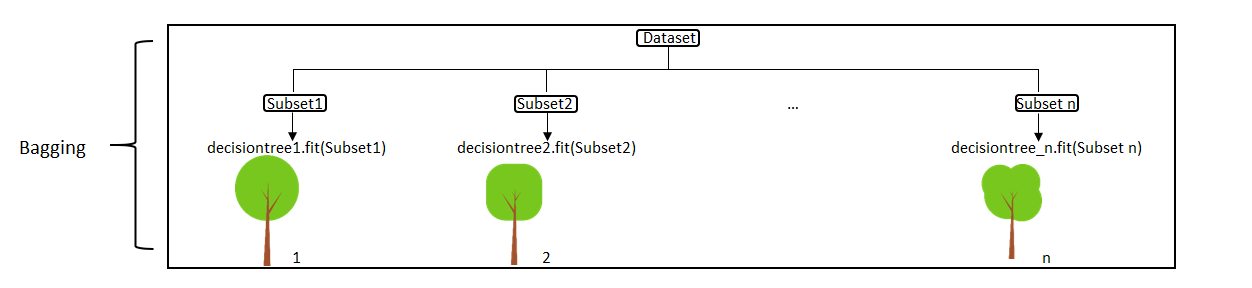
\includegraphics[width=16 cm]{images/bagging.png}
        \caption{Minh họa: Bagging}
        \label{fig:bagging}
    \end{figure}
    
    \subsubsection{Khái niệm: Random Forest}
    
    Random Forest \cite{breiman2001random}, hay còn gọi là Random Decision Forest, là một phương pháp ensemble, kết hợp nhiều mô hình cây quyết định phân lớp/hồi quy (Classification and regression trees - CART), cải tiến của phương pháp Bagging. RF được phát triển bởi Leo Breiman. Ông đồng thời cũng là tác giả của CART \cite{breiman_1984}
    
    \subsubsection{Mô tả thuật toán xây dựng Random Forest}
    
    \begin{itemize}
        \item Bước 1: Chọn ngẫu nhiên k từ n thuộc tính (k<n) có trong bộ dữ liệu huấn luyện.
        
        \item Bước 2: Sử dụng phương pháp boostrapping, chọn có hoàn lại từ bộ dữ liệu huấn luyện để tạo ra một bộ dữ liệu mới.
        
        \item Bước 3: Xây dựng cây quyết định với bộ dữ liệu ở bước 2, chỉ sử dụng k thuộc tính đã chọn ở bước 1
        
        \item Bước 4: Lặp lại Bước 2-3 để tạo nhiều cây quyết định khác.
        
        \item Bước 5: Kết hợp các cây quyết định thành phần bằng phương pháp bỏ phiếu.
    \end{itemize}
    
    \begin{figure}[htp]
        \centering
        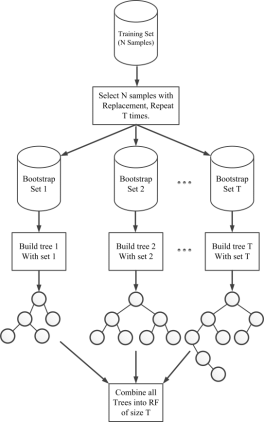
\includegraphics[width=8 cm, height=10cm]{images/Structure-of-random-forest.png}
        \caption{Minh họa: Random Forest \cite{RF_structure}}
        \label{fig:RF}
    \end{figure}
    
    \subsubsection{Dự đoán bằng Random Forest}
    
    Với x là một điểm dữ liệu mới, mỗi cây thành phần dự đoán hồi quy $T_{i}(x)$, dự đoán hồi quy của mô hình là:
    \begin{equation} \label{RF_reg}
        \hat{f}^{N}_{rf}(x) = \frac{1}{N} \underset{i=1}{ \overset{N}{\Sigma}} T_{i}(x)
    \end{equation}
    
    Với  $\hat{T}_{i}(x)$ là kết quả phân lớp của cây thành phần, dự đoán phân lớp của mô hình là:
    \begin{equation} \label{RF_cls}
        \hat{C}^{N}_{rf}(x) = majority \: vote \: \{\hat{T}_{i}(x)\}^{N}_{1}
    \end{equation}
    
    \subsubsection{Đánh giá Random Forest}
    
    Do sử dụng phương pháp boostrapping để tạo các mẫu huấn luyện cho các CART thành phần, chỉ có khoảng $\frac{2}{3}$ dữ liệu không trùng lặp trong bộ huấn luyện ban đầu được sử dụng cho việc huấn luyện. $\frac{1}{3}$ dữ liệu còn lại không tham gia huấn luyện được gọi là 'Out-of-bag dataset' (OOB). Phần dữ liệu này có thể xem như là một tập kiểm thử (validation dataset) dùng để đánh giá và tính toán độ quan trọng các thuộc tính của các CART trong rừng. Độ lỗi của RF trên tập dữ liệu OOB được gọi là 'Out-of-bag Error' ($E_{OOB}$).
    
    \begin{figure}[htp]
        \centering
        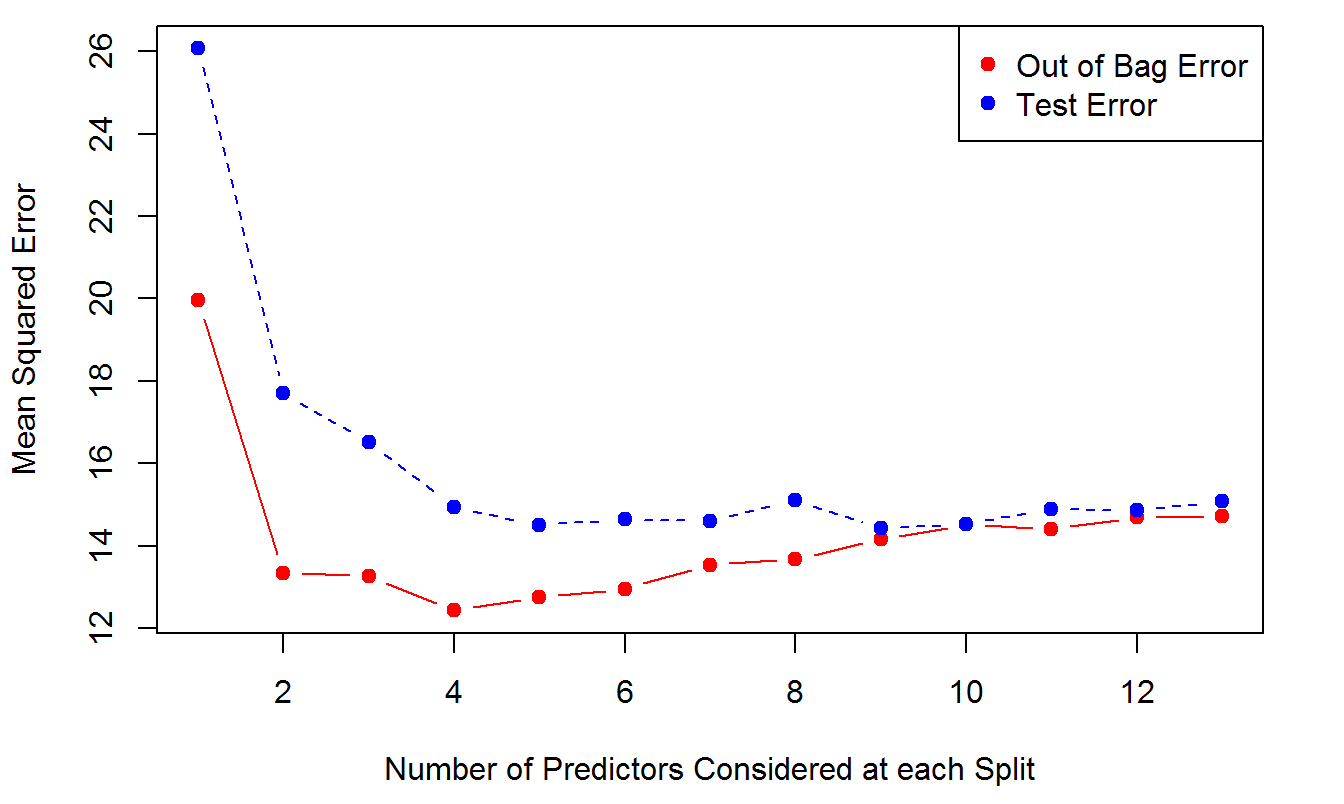
\includegraphics[width=12 cm]{images/rf_oob.png}
        \caption{Tương quan Out-of-bag error và test error}
        \label{fig:RF}
    \end{figure}
    
    Có thể so sánh $E_{OOB}$ giữa các RF có số thuộc tính được chọn k (ở bước 1) khác nhau và số lượng cây trong rừng khác nhau để chọn được mô hình RF có độ lỗi thấp nhất. 
    
    \subsubsection{Điểm mạnh của Random Forest}
    
    Thuật toán xây dựng có sự ngẫu nhiên trong mẫu dữ liệu (dùng phương pháp bootstrapping) và ngẫu nhiên trong số thuộc tính của mẫu so với tập thuộc tính ban đầu. Do đó, các tập huấn luyện con được tạo ra có tính đa dạng, ít liên quan. Mỗi CART xây dựng từ những tập dữ liệu con này không dùng tất cả dữ liệu training, cũng như không dùng tất cả các thuộc tính của dữ liệu để xây dựng nên mỗi cây có bias cao. Tuy nhiên, kết quả cuối của RF là kết hợp của nhiều cây thành phần, thông tin từ các cây sẽ bổ sung thông tin cho nhau, dẫn đến mô hình có low bias và low variance, tức là mô hình có kết quả dự đoán tốt.
    
    Trong rừng, mỗi cây thành phần chỉ được huấn luyện trên một tập nhỏ các thuộc tính thay vì toàn bộ (bước 1), cơ chế này giúp RF thực thi nhanh khi áp dụng trên tập dữ liệu có số lượng lớn thuộc tính. Hơn nữa, việc xây dựng từng cây thành phần là độc lập nên có thể dễ dàng thực hiện song song.


\subsection{Gradient Boosting (Tăng cường độ dốc)}
    \subsubsection{Khái niệm: Boosting}
        Boosting là một kỹ thuật ensemble với mục đích từ một số mô hình học yếu (weak learner) tạo ra mô hình học mạnh hơn (strong learner) bằng cách cho những mô hình sau sửa lỗi (học từ lỗi) của các mô hình trước. Các mô hình được thêm vào theo cách này cho đến khi đạt số lượng mô hình tối đa cho phép hoặc dự đoán hoàn toàn trùng khớp với tập huấn luyện.
        
        \begin{figure}[htp]
            \centering
            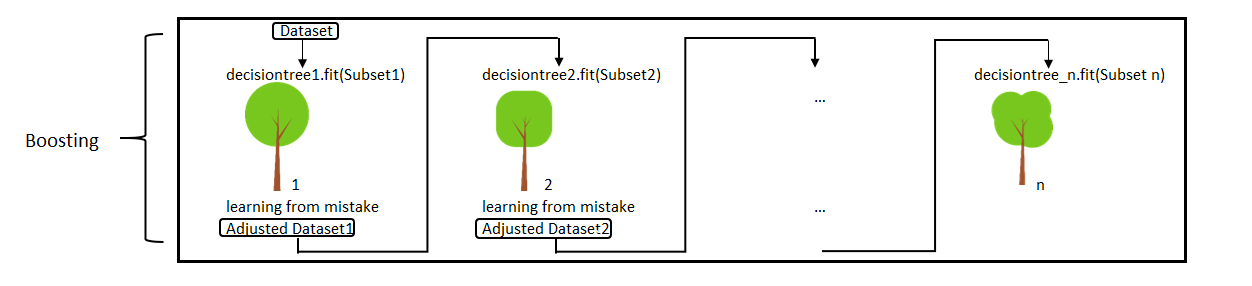
\includegraphics[width=16cm]{images/boosting.png}
            \caption{Minh họa: Boosting}
            \label{fig:boosting}
        \end{figure}
        
        Thuật toán boosting đơn giản nhất là Ada Boost, được giới thiệu vào năm 1995 bởi Freund và Schapire \cite{freund1997decision}.
        Thuật toán này sử dụng các CART có độ sâu nhỏ, hay còn gọi là một gốc (stump), làm các weak learner thành phần. 
        
        Ada Boost thực hiện việc học tăng cường bằng cách gán cho mỗi điểm dữ liệu trong bộ huấn luyện bộ huấn luyện một trọng số mẫu (sample wieght). Ban đầu, tất cả điểm dữ liệu đều được khởi tạo trọng số này bằng $\frac{1}{n}$, với n là tổng số điểm dữ liệu. Sau đó, với mỗi gốc được tạo, tổng lỗi của gốc đó sẽ quyết định trọng số của gốc trong việc bỏ phiếu (wieghted voting) cho kết quả dự đoán cuối. Những điểm dữ liệu cũng được cập nhật lại sample wieght dựa vào kết quả gốc hiện tại dự đoán đúng (sample wieght giảm) hay dự đoán sai (sample wieght tăng) thể hiện gốc sau đó cần dự thiết dự đoán đúng các điểm dữ liệu đang được dự đoán sai (gốc tiếp theo cố gắng sửa lỗi của gốc trước đó)
        
        Cụ thể thuật toán Ada Boost như sau \cite{freund1999short}:
        \begin{itemize}
            \item Khởi tạo $w_{1} = \{\frac{1}{N}\}^{N}_{1}$
            
            \item Với M là số gốc tối đa, lặp lại m=1,...M:
            \begin{itemize}
                \item Huấn luyện gốc sử dụng sample weight $w_{m}$
                
                \item Tính độ lỗi: 
                \begin{equation}
                    \epsilon_{t} = Pr_{i~D_{t}} [ h_{t} \ne y_{i} ]
                \end{equation}
                
                \item Thiết lập trọng số cho gốc này:
                    \begin{equation}
                        \alpha_{t} = \frac{1}{2}\ln{\frac{1 - \epsilon_{t}}{\epsilon_{t}}}
                    \end{equation}
                
                \item Cập nhật sample wieght cho việc huấn luyện gốc tiếp theo:
                    \begin{equation}
                        D_{t+1} = \frac{D_{t}(i)e^{-\alpha_{t}}}
                        {Z_{t}}
                    \end{equation}

                (với $Z_{t}$ là hệ số chuẩn hóa để tổng sample wieght bằng 1)
                
            \end{itemize}
            
            \item Cuối cùng, kết hợp các gốc bằng bỏ phiếu có trọng số:
                \begin{equation}
                    H(x) = sign( \underset{t=1}{ \overset{T}{\Sigma}} \alpha_{t} h_{t}(x) )
                \end{equation}
                \vspace{0.5cm}
    \clearpage
        \end{itemize}
        \clearpage
        \begin{figure}[H]
        \centering
        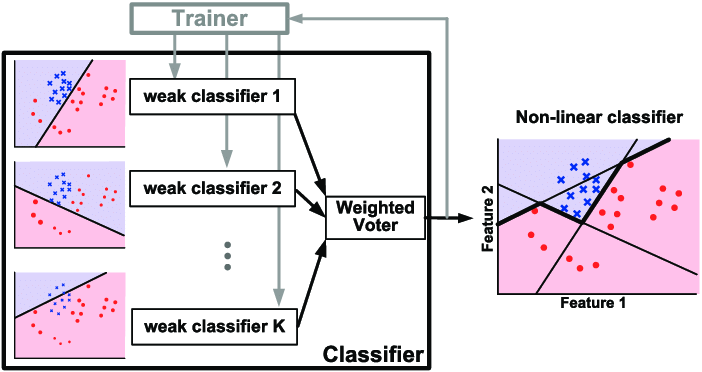
\includegraphics[width=8.5 cm,]{images/adaboost.png}
        \caption{Minh họa thuật toán AdaBoost, quá trình kết hợp các mô hình yếu \cite{adab_pic}}
        \label{fig:adab}
        \end{figure}
        
        
    \subsubsection{Gradient Boosting}
        Ý tưởng của thuật toán Gradient Boosting (GB) bắt nguồn từ Leo Breiman. Ông cho rằng phương pháp boosting có thể xem như là một thuật toán tối ưu hóa trên một hàm mất mát (Loss function) phù hợp \cite{breiman1997arcing}. Thuật toán Gradient boosting sau đó được phát triển bởi Jerome H. Friedman \cite{friedman2001greedy} \cite{friedman2002stochastic}.
        
        Khác với Ada Boost, ở Gradient Boosting:
            \begin{itemize}
                \item Sử dụng cây phân lớp, hồi quy làm các weaker learner thành phần thay vì gốc
            
                \item Những CART thành phần không huấn luyện dựa trên trọng số mẫu (mô hình tiếp theo cố gắng dự đoán đúng những điểm lỗi của mô hình trước), mà dựa trên  'độ lệch (lỗi) giả'(pseudo-residual) của CART tiền nhiệm trước đó (mô hình tiếp theo cố gắng giảm độ lỗi có được từ mô hình trước).
                
                \item Những mô hình thành phần không có trọng số riêng, thay vào đó chúng có chung một tỉ lệ tốc độ học (learning rate) trong khoảng {0-1} để điều chỉnh tốc độ học của từng mô hình mới.
            \end{itemize}
            
        Thuật toán kết thúc khi đạt số lượng cây tối đa hoặc việc thêm những cây mới không giảm pseudo-residual.
            
        \begin{figure}[htp]
        \centering
        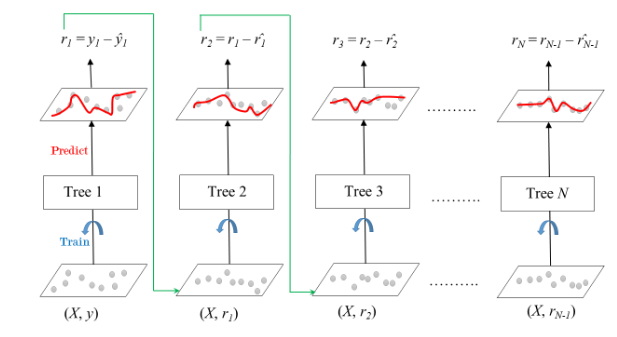
\includegraphics[width=10 cm,]{images/gradientboosting.png}
        \caption{Minh họa: Gradient boosting \cite{g4g_Gb}}
        \label{fig:gb}
        \end{figure}

        
    \subsubsection{Thuật toán Gradient Boosting \cite{starmer_2019_GBR} \cite{starmer_2019_GBC}:}
        
        Input: Dữ liệu huấn luyện $ \{(x_{i}, y_{i})\}^{n}_{i=1} $, một hàm Loss $ L(y, F(x)) $ và số lượng cây tối đa M
        \begin{itemize}
            \item Bước 1: Khởi tạo dự đoán ban đầu với hằng số
                \begin{equation}
                    F_{0}(x) = \underset{\gamma}{\mathrm{argmin}} \, 
                    \underset{i=1}{ \overset{n}{\Sigma}} L(y_{i}, \gamma)
                \end{equation}

            \item Bước 2: Lặp m=1 đến M để tạo M cây thành phần:
                \begin{description}
                    \item (A) Tính 'độ lệch giả' (pseudo-residual) của các điểm dữ liệu trong tập huấn luyện: Với mỗi i = 1, ..., n
                        \begin{equation}
                            r_{im} = -[\frac{\partial L(y_{i}, F(x_{i}))} {\partial F(x_{i})}]_{F(x) = F_{m-1}(x)}
                        \end{equation}
                        
                    \item (B) Xây dựng cây dự đoán các giá trị $r_{im}$, gọi $R_{jm}$ là các lá của cây, vớij=1, ...,$J_{m}$ (cây có $J_{m}$ lá)
                    
                    \item (C) Tính giá trị output ở từng lá của cây vừa tạo :
                        \begin{equation}
                            \gamma_{jm} = \underset{\gamma}{\mathrm{argmin}} \, 
                            \underset{x_{i} \in R_{ij}}{\Sigma}
                            L(y_{i}, F_{m-1}(x_{i}) + \gamma)
                        \end{equation}
                        
                    \item (D) Cập nhật dự đoán mới:
                        \begin{equation}
                            F_{m}(x) = F_{m-1}(x) + \nu \underset{j=1}{\overset{J_{m}}{\Sigma}}
                            \gamma_{m} I(x \in R{jm})
                        \end{equation}
                        với $\nu$ là tỷ lệ tốc độ học (learning rate)
                    
                \end{description}
                
        \end{itemize}
        
        Output: Kết quả dự đoán là kết quả của cây cuối cùng: $F_{M}(x)$
        
    \subsubsection{Điểm mạnh của Gradient Boosting}
        Qua mỗi cây mới được thêm vào, độ lỗi của mô hình sẽ ngày càng được giảm. Với các siêu tham số (hyperparameter) hợp lý, mô hình có thể cho được độ chính xác cao.
        
        \begin{figure}[htp]
        \centering
        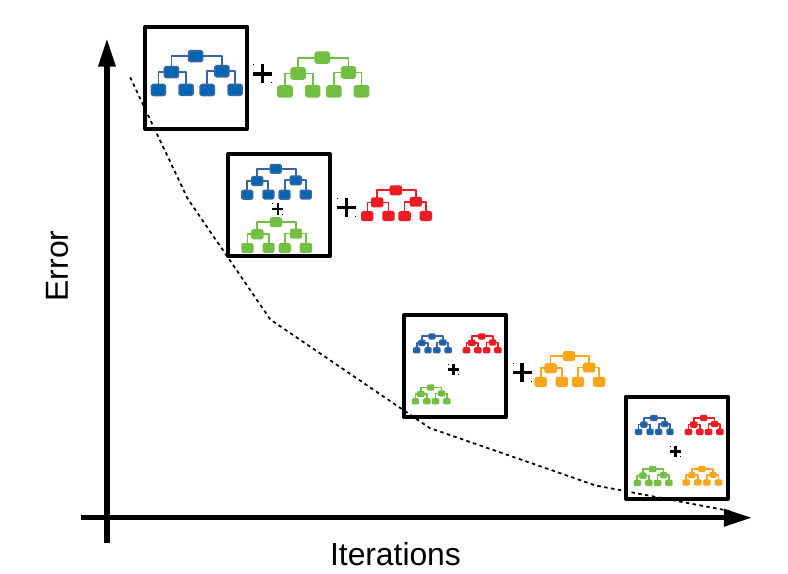
\includegraphics[width=10 cm,]{images/GB_error.png}
        \caption{Độ lỗi qua các iteration - GB \cite{gb_graph}}
        \label{fig:gb}
        \end{figure}
            
        Gradient Boosting có thể được tối ưu với nhiều hàm Loss khác nhau và cho phép hiệu chỉnh (fine tunning) nhiều siêu tham số (hyperparameter) giúp mô hình có độ linh hoạt cao giữa nhiều bộ dữ liệu khác nhau.


\subsection{XGBoost (Extreme Gradient Boosting)}
    XGBoost, viết tắt cho eXtreme Gradient Boosting, là một phiên bản Gradient Boosting được tối ưu hóa bởi Tianqi Chen \cite{chen2016xgboost}.
    
    Để cải tiến GB, mục tiêu của XGBoost không chỉ cố gắng tối thiểu hóa hàm Loss mà còn kèm theo một hàm chính quy hóa (regularization). Ta có thể gọi hàm mục tiêu (objective function) của XGBoost là: \cite{xgboost_model_tut}
    \begin{equation}
        obj(\theta) = \underset{i=1}{\overset{n}{\Sigma}} L(y_{i}, \hat{y}_{i}) + \underset{k=1}{\overset{K}{\Sigma}} \Omega(f_{k}) 
    \end{equation}
    với L là hàm Loss, $\Omega$ là hàm regularization, $f_{k}$ là mô hình thành phần thứ k. Việc thêm hàm regularization giúp cải tiến vấn đề overfit của mô hình Gradient Boosting, do sau mỗi lần thêm cây thành phần, độ lỗi của mô hình GB luôn được giảm cho đến tối thiểu hoặc mô hình đạt tối đa số cây thành phần.
    
    \subsubsection{Xây dựng CART trong mô hình XGBoost}
    Một trong những cải tiến của XGBoost so với Gradient Boost là ở việc tạo các cây hồi quy/phân lớp thành phần.
    
    Ở iteration thứ t, cây được tạo cho dự đoán 
    \begin{equation}
        \hat{y}_{i}^{(t)} =  \hat{y}_{i}^{(t-1)} + f_{t} (x_{i}) = \underset{k=1}{\overset{T}{\Sigma}}\Omega(f_{k}(x_{i}))
    \end{equation}
    
    Độ phức tạp của cây được định nghĩa là \cite{xgboost_model_tut}
    \begin{equation}
        \Omega(f) = \gamma T + \frac{1}{2} \lambda \underset{j=1}{\overset{T}{\Sigma}} w^{2}_{j}
    \end{equation}
    với $\gamma$ và $\lambda$ là các hệ số regularization, T là số lá của cây. Ta thấy $\underset{j=1}{\overset{T}{\Sigma}}w^{2}_{j}$ là tổng bình phương các lá, hay chính là tổng bình phương output của cây. Ta có thể đặt:
    
    \begin{equation}
        O^{2}_{value} = f_{t} (x_{i})^2 = \underset{j=1}{\overset{T}{\Sigma}}w^{2}_{j}
    \end{equation}
    
    khi đó độ phức tạp của cây là:
    \begin{equation}
        \Omega(f) = \gamma T + \frac{1}{2} \lambda  O^{2}_{value}
    \end{equation}
    
    Lúc này, hàm mục tiêu của XGBoost là \cite{xgboost_model_tut} \cite{starmer_2020_XGB}
    \begin{equation}
    \begin{split}
         obj^{(t)} & =  \underset{i=1}{\overset{n}{\Sigma}} L(y_{i}, \hat{y}_{i}^{(t-1)} + f_{t} (x_{i})) 
            + \Omega(f_{t}) + constant \\
           & = \underset{i=1}{\overset{n}{\Sigma}} L(y_{i}, \hat{y}_{i}^{(t-1)} + O_{value}) 
            + \gamma T + \frac{1}{2} \lambda  O^{2}_{value} + constant
    \end{split}
    \end{equation}
    
    Vậy, XGBoost chỉ thêm cây có output làm tối thiểu hóa được hàm mục tiêu này. Các hằng số sẽ không ảnh hưởng đến bài toán tối thiểu hóa nên ta có thể bỏ chúng đi
    \begin{equation}
         obj^{(t)} = \underset{i=1}{\overset{n}{\Sigma}} L(y_{i}, \hat{y}_{i}^{(t-1)} + O_{value}) 
         + \frac{1}{2} \lambda  O^{2}_{value}
    \end{equation}
    
    Áp dụng xấp xỉ Taylor bậc 2 (second order Taylor Approximation) \cite{Taylor_theorem}:
    
    \begin{equation}
    \begin{split}
        L(y_{i}, \hat{y}_{i}^{(t-1)} + O_{value}) \approx 
        L(y_{i}, \hat{y}_{i}^{(t-1)})
        & + \left[ \frac{d}{ d_{\hat{y}_{i}^{(t-1)}}}  L(y_{i}, \hat{y}_{i}^{(t-1)}) \right] O_{value} \\
        & + \frac{1}{2} \left[ \frac{d^{2}}{d^{2}_{\hat{y}_{i}^{(t-1)}}}  L(y_{i}, \hat{y}_{i}^{(t-1)}) \right] O^2_{value}
    \end{split}
    \end{equation}
    
    Đặt
    \begin{equation}
    \begin{split}
        & g = \left[ \frac{d}{ d_{\hat{y}_{i}^{(t-1)}}}  L(y_{i}, \hat{y}_{i}^{(t-1)}) \right]
        \\
        & h = \left[ \frac{d^{2}}{d^{2}_{\hat{y}_{i}^{(t-1)}}}  L(y_{i}, \hat{y}_{i}^{(t-1)}) \right]
    \end{split}
    \end{equation}
    
    Khi đó, hàm mục tiêu có thể được viết thành 
    \begin{equation}
        obj^{(t)} = \underset{i=1}{\overset{n}{\Sigma}} L(y_{i}, \hat{y}_{i}^{(t-1)})
        + \underset{i=1}{\overset{n}{\Sigma}} g_{i} O_{value}
        + \frac{1}{2} \underset{i=1}{\overset{n}{\Sigma}} h_{i} O^2_{value}
        + \frac{1}{2} \lambda O^2_{value}
    \end{equation}
    
    Ta thấy được $\underset{i=1}{\overset{n}{\Sigma}} L(y_{i}, \hat{y}_{i}^{(t-1)}) $ không chứa $O_{value}$, nên nó sẽ không ảnh hưởng đến quá trình tối thiểu hóa và có thể được bỏ đi. Hàm mục tiêu bây giờ là
    
    \begin{equation} \label{obj_func}
         obj^{(t)} = O_{value} \underset{i=1}{\overset{n}{\Sigma}} g_{i}
         + \frac{1}{2} O^2_{value} (\underset{i=1}{\overset{n}{\Sigma}} h_{i} + \lambda)
    \end{equation}
    
    Để tìm $O_{value}$ làm tối thiểu hàm mục tiêu, ta lấy đạo hàm hàm mục tiêu theo $O_{value}$ và tìm nghiệm bằng 0:
    
    \begin{equation} \label{eq_Ovalue}
        \begin{split}
            & \underset{i=1}{\overset{n}{\Sigma}} g_{i}
            + O_{value} (\underset{i=1}{\overset{n}{\Sigma}}h_{i} + \lambda) = 0 \\ \\
           	\Leftrightarrow \; &  O_{value} = - \frac{\underset{i=1}{\overset{n}{\Sigma}} g_{i}} {\underset{i=1}{\overset{n}{\Sigma}}h_{i} + \lambda}
        \end{split}
    \end{equation}
    
    \textbf{Ở bài toán hồi quy}, giả sử ta sử dụng hàm Loss MSE 
    $ L(y_{i}, \hat{y}_{i}^{(t-1)}) = \frac{1}{2} (y_{i} - \hat{y}_{i}^{(t-1)})^2 $, ta có thể tính $g_{i}$ và $h_{i}$
    \begin{equation}
        \begin{split}
        & g = -(y_{i} - \hat{y}_{i}^{(t-1)})
        \\
        & h = 1
        \end{split}
    \end{equation}
    
    thì hàm mục tiêu là:
    \begin{equation}
        O_{value} = \frac{\underset{i=1}{\overset{n}{\Sigma}} (y_{i} - \hat{y}_{i}^{(t-1)})}
        {\underset{i=1}{\overset{n}{\Sigma}}1 + \lambda}
    \end{equation}
    
    Ta thấy được ở phân số trên, tử số chính là tổng độ lỗi (sum of residuals) và mẫu số chính là tổng số phần tử trong kết quả (number of residuals) trong output + $\lambda$
    
    Vậy hàm mục tiêu của mô hình hồi quy này có thể hiểu là \cite{starmer_2020_XGB}
    \begin{equation}
        O_{value} = \frac{\text{Sum of Residuals}}
        {\text{Number of Residuals} + \lambda}
    \end{equation}
    
    Đây chính là công thức kết quả của một lá trên cây hồi quy.
    
    \textbf{Ở bài toán phân lớp}, giả sử ta sử dụng hàm Loss
    \begin{equation}
        L(y_{i}, \hat{y}_{i}^{(t-1)}) = -[ y_{i} \log(\hat{y}_{i}^{(t-1)}) + (1-y_{i})\log(1-\hat{y}_{i}^{(t-1)})]
    \end{equation}
    
    ta có thể tính $g_{i}$ và $h_{i}$ \cite{starmer_2020_XGB}
    \begin{equation}
        \begin{split}
        & g = -(y_{i} - \hat{y}_{i}^{(t-1)})
        \\
        & h = \hat{y}_{i}^{(t-1)}(1 - \hat{y}_{i}^{(t-1)})
        \end{split}
    \end{equation}
    
    thì hàm mục tiêu là:
    \begin{equation}
        O_{value} = \frac{\underset{i=1}{\overset{n}{\Sigma}} (y_{i} - \hat{y}_{i}^{(t-1)})}
        {\underset{i=1}{\overset{n}{\Sigma}}(\hat{y}_{i}^{(t-1)}(1 - \hat{y}_{i}^{(t-1)})) + \lambda}
    \end{equation}
    
    hay dễ hiểu chính là: \cite{starmer_2020_XGB}
    \begin{equation}
        O_{value} = \frac{\text{Sum of Residuals}}
        {\Sigma\text{[Previous Probability x (1 - Previous Probability)]} + \lambda}
    \end{equation}
    
    Đây chính là công thức kết quả của một lá trên cây phân lớp.
    
    \bigbreak
    
    \textbf{Tách lá ở cây}
    
    Ở XGBoost, khi tách một lá, ta dùng hàm Gain để xác định xem các cây con mới này phân cụm tốt hơn lá ban đầu hay không.
    \begin{equation} \label{eq_XBG_gain}
        \begin{split}
        \text{Gain} = \: & \text{Similarity Score}(\text{Lá trái}) 
        + \text{Similarity Score}(\text{Lá phải}) \\
        & - \text{Similarity Score}(\text{Gốc}) - \gamma
        \end{split}
    \end{equation}
    và tất nhiên cây con có Gain lớn nhất sẽ được chọn để tách lá.
    
    Công thức của Similarity Score (được miêu tả trong bản thảo XGBoost ban đầu \cite{chen2016xgboost}) ở hàm Gain trong XGBoost chính là âm của hàm mục tiêu đã được tối thiểu hóa.Tức là, để tính công thức Similarity Score, ta thế đáp án $O_{value}$ ta tính được ở \eqref{eq_Ovalue} vào \eqref{obj_func}
    \begin{equation}
        \begin{split}
        \text{Similarity Score} & = - \underset{i=1}{\overset{n}{\Sigma}} g_{i} (- \frac{\underset{i=1}{\overset{n}{\Sigma}} g_{i}} {\underset{i=1}{\overset{n}{\Sigma}}h_{i} + \lambda})
         - \frac{1}{2} (\underset{i=1}{\overset{n}{\Sigma}} h_{i} + \lambda) (- \frac{\underset{i=1}{\overset{n}{\Sigma}} g_{i}} {\underset{i=1}{\overset{n}{\Sigma}}h_{i} + \lambda})^2
        \\
        & = \frac{1}{2} \frac{(\underset{i=1}{\overset{n}{\Sigma}} g_{i})^2} {\underset{i=1}{\overset{n}{\Sigma}} h_{i} + \lambda}
        \end{split}
    \end{equation}
    Tuy nhiên, do Similarity Score là tương đối giữa các cây con và để giảm số tính toán cần thiết (tối ưu hóa), Similarity Score được áp dụng thực tế được bỏ đi phần $\frac{1}{2}$
    \begin{equation} \label{eq_XGB_sim}
        \text{Similarity Score} =  \frac{(\underset{i=1}{\overset{n}{\Sigma}} g_{i})^2} {\underset{i=1}{\overset{n}{\Sigma}} h_{i} + \lambda}
    \end{equation}
    
    Tương tự như cách tính $O_{value}$ cho bài toán hồi quy và phân lớp đã nêu ở trên, ta có thể tính được hàm Similarity Score với các hàm Loss khác nhau. Giả sử bài toán hồi quy và phần lớp sử dụng hàm Loss nêu trên, ta có thể tính hàm Similarity Score:
    
    \begin{equation}
        \text{Similarity Score} = \frac{(\underset{i=1}{\overset{n}{\Sigma}} (y_{i} - \hat{y}_{i}^{(t-1)}))^2}
        {\underset{i=1}{\overset{n}{\Sigma}}1 + \lambda}
    \end{equation}
    
    hay dễ hiểu chính là: \cite{starmer_2020_XGB}
    \begin{equation}
        \text{Similarity Score} = \frac{\text{(Sum of Residuals)}^2}
        {\text{Number of Residuals} + \lambda}
    \end{equation}
    
    cho hồi quy, và
    
    \begin{equation}
        \text{Similarity Score} = \frac{(\underset{i=1}{\overset{n}{\Sigma}} (y_{i} - \hat{y}_{i}^{(t-1)}))^2}
        {\underset{i=1}{\overset{n}{\Sigma}}(\hat{y}_{i}^{(t-1)}(1 - \hat{y}_{i}^{(t-1)})) + \lambda}
    \end{equation}
    
    hay dễ hiểu chính là: \cite{starmer_2020_XGB}
    \begin{equation}
        \text{Similarity Score} = \frac{\text{(Sum of Residuals)}^2}
        {\Sigma\text{[Previous Probability x (1 - Previous Probability)]} + \lambda}
    \end{equation}
    
    cho phân lớp.
    
    \bigbreak
    
    \textbf{Tỉa cành cây}
    
    Quay lại với hàm Gain \eqref{eq_XBG_gain} sau khi ta đã tính được công thức của Similariry Score \eqref{eq_XGB_sim}
    
    \begin{equation} \label{eq_XGB_Gain_final}
        \text{Gain} = \: \frac{(\underset{i=1}{\overset{n}{\Sigma}} g^{\text{Lá trái}}_{i})^2} {\underset{i=1}{\overset{n}{\Sigma}} h^{\text{Lá trái}}_{i} + \lambda} 
        + \frac{(\underset{i=1}{\overset{n}{\Sigma}} g^{\text{Lá phải}}_{i})^2} {\underset{i=1}{\overset{n}{\Sigma}} h^{\text{Lá phải}}_{i} + \lambda} 
        - \frac{(\underset{i=1}{\overset{n}{\Sigma}} g^{\text{Ngọn}}_{i})^2} {\underset{i=1}{\overset{n}{\Sigma}} h^{\text{Ngọn}}_{i} + \lambda} - \gamma
    \end{equation}
    
    Khi đã xây dựng xong cây, từ dưới lên trên, những nút đã tách lá nhưng cho Gain nhỏ hơn 0 sẽ bị 'tỉa cảnh' (tree pruning), gộp lại hai lá mà nút đó đã tách thành trở về một nút ban đầu. Tỉa cành ở đây giúp giảm độ phức tạp của các cây thành phần (regularization), giúp XGBoost giảm overfit
    
    Dựa vào công thức hàm Gain \eqref{eq_XGB_Gain_final}, ta thấy được hệ số regularization $\lambda$ và $\alpha$ càng cao thì việc tỉa cành sẽ càng mạnh.
    
\subsection {Logistic Classification (Hồi quy Logistic)}
\label{label:log_class}

Hồi quy Logistic (Logistic Regression) là một mô hình học máy tuyến tính dùng để giải quyết các bài toán \textbf{phân loại nhị phân}, trong đó đầu ra là một biến phân loại có hai trạng thái (ví dụ: 0/1, âm tính/dương tính).

\textbf{Ý tưởng chính}

Thay vì dự đoán một giá trị liên tục như hồi quy tuyến tính, Logistic Regression dự đoán xác suất một điểm dữ liệu thuộc về lớp dương (lớp 1), bằng cách sử dụng hàm sigmoid để biến đổi đầu ra thành giá trị trong khoảng \([0, 1]\).

\textbf{Công thức mô hình}

Cho đầu vào \( \mathbf{x} = (x_1, x_2, \ldots, x_n)^T \), và vector trọng số \( \mathbf{w} = (w_0, w_1, \ldots, w_n)^T \):

\begin{itemize}
    \item \textbf{Hàm dự đoán (sigmoid)}:
    \[
    \hat{y} = \sigma(z) = \frac{1}{1 + e^{-z}}, \quad \text{với } z = \mathbf{w}^T \mathbf{x} + b
    \]
    \item \textbf{Quy tắc phân loại}:
    \[
    \hat{y} \geq 0.5 \Rightarrow \text{lớp 1}; \quad \hat{y} < 0.5 \Rightarrow \text{lớp 0}
    \]
\end{itemize}

\textbf{Hàm mất mát (Binary Cross-Entropy)}

Hàm mất mát dùng để huấn luyện mô hình là:

\[
\mathcal{L}(\mathbf{w}) = -\frac{1}{m} \sum_{i=1}^{m} \left[ y^{(i)} \log \hat{y}^{(i)} + (1 - y^{(i)}) \log (1 - \hat{y}^{(i)}) \right]
\]

Trong đó:
\begin{itemize}
    \item \( m \): số mẫu trong tập huấn luyện
    \item \( y^{(i)} \): nhãn thực tế của mẫu thứ \( i \)
    \item \( \hat{y}^{(i)} \): xác suất dự đoán của mẫu thứ \( i \)
\end{itemize}

\textbf{Huấn luyện mô hình}

Trọng số \( \mathbf{w} \) được cập nhật qua thuật toán tối ưu như:
\begin{itemize}
    \item Gradient Descent
    \item Stochastic Gradient Descent
    \item Hoặc các trình tối ưu hóa hiện đại (Adam, RMSprop,...)
\end{itemize}

\textbf{Ưu điểm}

\begin{itemize}
    \item Mô hình đơn giản, dễ hiểu và dễ triển khai.
    \item Dự đoán xác suất thay vì chỉ nhãn.
    \item Hoạt động tốt với dữ liệu tuyến tính.
\end{itemize}

\textbf{Nhược điểm}

\begin{itemize}
    \item Không xử lý tốt các quan hệ phi tuyến (non-linear).
    \item Nhạy cảm với dữ liệu mất cân bằng giữa các lớp.
\end{itemize}

\textbf{Ứng dụng}

\begin{itemize}
    \item Phân loại email spam / không spam.
    \item Dự đoán khả năng khách hàng rời đi (churn prediction).
    \item Chẩn đoán y tế (ví dụ: bệnh có/không).
    \item Phân tích rủi ro tài chính (nợ xấu, vỡ nợ).
\end{itemize}

\subsection {K-Nearest Neighbors - KNN (Láng giềng gần nhất)}
\label{label:knn}

K-Nearest Neighbors (KNN) là một thuật toán học máy không tham số (non-parametric), sử dụng khoảng cách để phân loại hoặc dự đoán một điểm dữ liệu mới dựa trên các điểm gần nhất trong tập huấn luyện.

\textbf{Nguyên lý hoạt động}

\begin{enumerate}
    \item Tính khoảng cách từ điểm cần phân loại đến tất cả các điểm trong tập huấn luyện.
    \item Chọn ra \(k\) điểm gần nhất (nearest neighbors).
    \item Dự đoán nhãn của điểm mới dựa trên đa số nhãn (phân loại) hoặc trung bình (hồi quy) của \(k\) điểm gần nhất.
\end{enumerate}

\textbf{Công thức tính khoảng cách}

Phổ biến nhất là khoảng cách Euclid:

\[
d(\mathbf{x}, \mathbf{x}^{(i)}) = \sqrt{ \sum_{j=1}^n \left( x_j - x_j^{(i)} \right)^2 }
\]

Các lựa chọn khác:
\begin{itemize}
    \item Khoảng cách Manhattan:
    \[
    d(\mathbf{x}, \mathbf{x}^{(i)}) = \sum_{j=1}^n \left| x_j - x_j^{(i)} \right|
    \]
    \item Khoảng cách Minkowski (tổng quát):
    \[
    d(\mathbf{x}, \mathbf{x}^{(i)}) = \left( \sum_{j=1}^n \left| x_j - x_j^{(i)} \right|^p \right)^{1/p}
    \]
\end{itemize}

\textbf{Quy tắc phân loại}

\[
\hat{y} = \text{mode} \left( y^{(i_1)}, y^{(i_2)}, \dots, y^{(i_k)} \right)
\]

Trong đó:
\begin{itemize}
    \item \( \hat{y} \): nhãn dự đoán
    \item \( y^{(i)} \): nhãn của điểm lân cận thứ \(i\)
\end{itemize}

\textbf{Ưu điểm}

\begin{itemize}
    \item Dễ cài đặt và trực quan.
    \item Không cần huấn luyện mô hình (lazy learning).
    \item Phù hợp với bài toán phi tuyến.
\end{itemize}

\subsection*{Nhược điểm}

\begin{itemize}
    \item Tính toán chậm với dữ liệu lớn (phải tính khoảng cách với tất cả điểm huấn luyện).
    \item Nhạy cảm với nhiễu và thang đo dữ liệu (cần chuẩn hóa).
    \item Chọn \(k\) không phù hợp có thể gây quá khớp hoặc dưới khớp.
\end{itemize}

\textbf{Ứng dụng}

\begin{itemize}
    \item Nhận diện chữ viết tay (như MNIST).
    \item Dự đoán người dùng giống nhau trong hệ thống gợi ý.
    \item Phân loại bệnh, dữ liệu gen, khách hàng,...
\end{itemize}

\subsection {K-Means (Thuật toán phân cụm K trung bình)}
\label{label:kmean}
K-Means là một thuật toán học không giám sát phổ biến \cite{bishop2006pattern}, được sử dụng rộng rãi trong các bài toán phân cụm dữ liệu. Mục tiêu của K-Means là chia tập dữ liệu thành \textbf{K cụm} sao cho các điểm dữ liệu trong cùng một cụm có độ tương đồng cao với nhau và khác biệt rõ ràng với các cụm còn lại.

\subsubsection*{Nguyên lý hoạt động}

Thuật toán hoạt động theo các bước chính sau:

\begin{enumerate}
    \item \textbf{Khởi tạo:} Chọn ngẫu nhiên $K$ tâm cụm ban đầu (centroids).
    \item \textbf{Phân cụm:} Gán mỗi điểm dữ liệu vào cụm có tâm gần nhất (theo khoảng cách Euclidean).
    \item \textbf{Cập nhật:} Tính lại vị trí tâm cụm mới bằng trung bình các điểm trong cụm.
    \item \textbf{Lặp lại:} Quay lại bước 2 và 3 cho đến khi các tâm cụm hội tụ (không thay đổi đáng kể) hoặc đạt số vòng lặp tối đa.
\end{enumerate}

\subsubsection*{Công thức khoảng cách Euclidean}

Khoảng cách giữa điểm dữ liệu $x$ và tâm cụm $c$ được tính bằng công thức:

\[
d(x, c) = \sqrt{\sum_{i=1}^{n} (x_i - c_i)^2}
\]

Trong đó:
\begin{itemize}
    \item $x$: điểm dữ liệu.
    \item $c$: tâm cụm.
    \item $n$: số chiều của không gian dữ liệu.
\end{itemize}

\subsubsection*{Tham số quan trọng}

\begin{itemize}
    \item \textbf{K:} Số lượng cụm cần phân chia (phải được xác định trước).
    \item \textbf{Max iterations:} Số vòng lặp tối đa để thuật toán hội tụ.
    \item \textbf{Tolerance:} Ngưỡng thay đổi của tâm cụm để quyết định dừng thuật toán.
\end{itemize}

\subsubsection*{Ưu điểm}

\begin{itemize}
    \item Dễ hiểu và dễ triển khai.
    \item Tính toán nhanh, đặc biệt với dữ liệu lớn.
\end{itemize}

\subsubsection*{Hạn chế}

\begin{itemize}
    \item Nhạy cảm với vị trí khởi tạo tâm cụm.
    \item Phải biết trước số cụm $K$.
    \item Không hoạt động tốt với dữ liệu có hình dạng phức tạp hoặc phân bố chồng lấn.
\end{itemize}

\subsubsection*{Ứng dụng}

\begin{itemize}
    \item Phân đoạn khách hàng (customer segmentation).
    \item Nhóm ảnh trong xử lý ảnh (image clustering).
    \item Nhận dạng mẫu (pattern recognition).
    \item Nén ảnh (image compression).
\end{itemize}

\subsection {Spectral Clustering (Phân cụm phổ)}
\label{label:SpectralClustering}

Spectral Clustering (phân cụm phổ) \cite{868688} là một thuật toán phân cụm tiên tiến dựa trên lý thuyết đồ thị và đại số tuyến tính. Thay vì phân cụm trực tiếp trên không gian dữ liệu, thuật toán này chuyển dữ liệu sang một không gian mới thông qua việc phân tích các giá trị riêng (eigenvalues) và vector riêng (eigenvectors) của một ma trận biểu diễn quan hệ giữa các điểm dữ liệu.

\subsubsection*{Nguyên lý hoạt động}

Spectral Clustering hoạt động thông qua các bước chính sau:

\begin{enumerate}
    \item \textbf{Xây dựng ma trận kề (Adjacency Matrix)}: Xác định mức độ liên kết giữa các điểm dữ liệu (thường dùng khoảng cách Gaussian hoặc k-NN).
    \item \textbf{Tính ma trận Laplacian}: Từ ma trận kề, tính ma trận Laplacian $L = D - A$, trong đó $D$ là ma trận bậc (degree matrix) và $A$ là ma trận kề.
    \item \textbf{Phân tích giá trị riêng}: Tính các vector riêng tương ứng với $k$ giá trị riêng nhỏ nhất (hoặc lớn nhất tuỳ loại Laplacian).
    \item \textbf{Ánh xạ không gian mới}: Biểu diễn mỗi điểm dữ liệu theo các vector riêng.
    \item \textbf{Áp dụng phân cụm K-Means}: Áp dụng thuật toán K-Means trong không gian mới này để phân chia cụm.
\end{enumerate}

\subsubsection*{Ưu điểm}
\begin{itemize}
    \item Phân cụm tốt cho dữ liệu có hình dạng phức tạp, không lồi.
    \item Không yêu cầu giả định phân phối dữ liệu.
    \item Có thể áp dụng cho dữ liệu biểu diễn dưới dạng đồ thị.
\end{itemize}

\subsubsection*{Hạn chế}
\begin{itemize}
    \item Hiệu suất kém với dữ liệu lớn (do tính toán ma trận và phân tích trị riêng).
    \item Cần chọn tham số phù hợp: số cụm $k$, hàm tương đồng, và tham số Gaussian $\sigma$.
\end{itemize}

\subsubsection*{Ứng dụng}
\begin{itemize}
    \item Phân tích mạng xã hội.
    \item Phân đoạn ảnh trong thị giác máy tính.
    \item Nhận dạng cộng đồng (community detection) trong đồ thị.
\end{itemize}

\subsection {Gaussian Mixture Model - GMM (Mô hình hỗn hợp Gauss)}
\label{label:SpectralClustering}

Gaussian Mixture Model (GMM) \cite{bishop2006pattern} là một mô hình xác suất dùng để biểu diễn sự phân bố của dữ liệu như là sự kết hợp của nhiều phân phối Gaussian (chuẩn) khác nhau. GMM là một phương pháp phân cụm dựa trên mô hình (model-based clustering), cho phép mô hình hóa các cụm có hình dạng ellipsoid và phân bố chồng lấn.

\subsubsection*{Nguyên lý hoạt động}

GMM giả định rằng dữ liệu được tạo ra từ sự kết hợp của $K$ phân phối Gaussian. Mỗi điểm dữ liệu có xác suất thuộc về mỗi Gaussian khác nhau, thay vì gán cứng vào một cụm như K-Means.

Xác suất tổng hợp của một điểm dữ liệu $x$ là:

\[
p(x) = \sum_{k=1}^{K} \pi_k \cdot \mathcal{N}(x \mid \mu_k, \Sigma_k)
\]

Trong đó:
\begin{itemize}
    \item $\pi_k$: trọng số (mixing coefficient) của thành phần thứ $k$ ($\sum \pi_k = 1$).
    \item $\mu_k$: vector trung bình của phân phối Gaussian thứ $k$.
    \item $\Sigma_k$: ma trận hiệp phương sai của phân phối Gaussian thứ $k$.
    \item $\mathcal{N}(x \mid \mu_k, \Sigma_k)$: phân phối chuẩn đa biến.
\end{itemize}

\subsubsection*{Thuật toán ước lượng tham số: EM (Expectation-Maximization)}

\begin{enumerate}
    \item \textbf{E-step (Expectation):} Tính xác suất mỗi điểm thuộc về từng thành phần Gaussian (trách nhiệm).
    \item \textbf{M-step (Maximization):} Cập nhật các tham số $\pi_k$, $\mu_k$, và $\Sigma_k$ để cực đại hóa log-likelihood.
    \item \textbf{Lặp lại} cho đến khi hội tụ.
\end{enumerate}

\subsubsection*{Ưu điểm}

\begin{itemize}
    \item Mô hình được các cụm phức tạp hơn hình cầu (so với K-Means).
    \item Gán mềm (soft clustering), mỗi điểm có thể thuộc nhiều cụm với các xác suất khác nhau.
\end{itemize}

\subsubsection*{Hạn chế}

\begin{itemize}
    \item Nhạy cảm với khởi tạo ban đầu.
    \item Dễ bị rơi vào cực trị cục bộ.
    \item Hiệu suất giảm với dữ liệu có chiều cao.
\end{itemize}

\subsubsection*{Ứng dụng}

\begin{itemize}
    \item Nhận dạng giọng nói và âm thanh.
    \item Phân đoạn ảnh (image segmentation).
    \item Hệ thống khuyến nghị.
    \item Phát hiện dị thường (anomaly detection).
\end{itemize}

\subsection{LSTM (Long Short-Term Memory)}
    \subsubsection{Artificial Neural Network (ANN)}
    Artificial Neural Network hay mạng thần kinh nhân tạo, gọi tắt là mạng thần kinh hoặc mạng neural, là một mô hình xử lý thông tin lấy cảm hứng từ  mạng neural sinh học. Kiến trúc của một mạng neural gồm 3 thành phần đó là lớp vào - input layer, lớp ẩn - hidden layer và lớp ra - output layer. Lưu ý, một mạng neural có thể chứa nhiều lớp ẩn ở giữa lớp vào và lớp ra.
    \begin{figure}[htp]
        \centering
        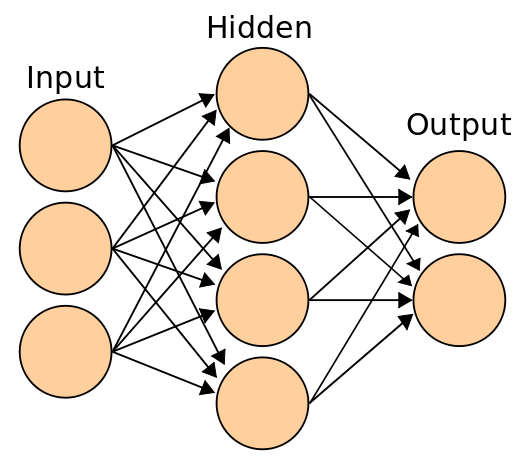
\includegraphics[width=6 cm]{images/ann.png}
        \caption{Minh họa cấu trúc của một mạng neural. \cite{ann_struct}}
        \label{fig:ann_structure}
    \end{figure}
    
    Ta có thể mô tả hoạt động mạng neural bằng công thức
    \begin{equation} \label{ann_eqn}
        y^{(l)}_i = f^{(l)}_i\left(\sum_{j=1}^{n^{(l-1)}}w^{(l)}_{ij}y^{(l-1)}_{j} + b^{(l)}_i\right).
    \end{equation}
    Trong đó:
    \begin{itemize}
        \item $l=1\dotsc L$, với $L$ là số lớp của mạng và $n^l$ là số neural ở lớp thứ $l$.
        \item $y^{(l)}_i$ là đầu ra của neural thứ $i$ ở lớp thứ $l$, với $i = 1\dotsc n^{l}$.
        \item $f^{(l)}_i$ là hàm truyền của neural thứ $i$ ở lớp thứ $l$. Hàm truyền tồn tại nhiều lựa chọn và mỗi lựa chọn có ảnh hưởng lớn đến kết quả đầu ra của mạng.
        \item $w_{i}^{(l)}$ là trọng số của đầu vào thứ $i$ ở lớp thứ $l$ thể hiện độ mạnh của từng đầu vào đối với quá trình xử lý thông tin để chuyển đổi dữ liệu từ lớp này sang lớp khác.
        \item Đầu vào của mạng là $y^{(0)} = \textbf{x}$ và đầu ra cuối là $\textbf{y} = y^{(L)}$.
        \item $b^{(l)}_i$ là \textit{ngưỡng} (bias) của neural thứ $i$ ở lớp thứ $l$.
    \end{itemize}
    
    Như vậy, quá trình học của mạng neural là quá trình tìm bộ trọng số $\textbf{w}$ sao cho phù hợp nhất. Quá trình này sẽ lặp liên tục và có thể không dừng đến khi tìm ra kết quả như ý. Vì vậy, trong thực tế, khi huấn luyện một mô hình mạng neural, một tiêu chuẩn dựa trên một giá trị sai số nào giữa đầu ra của mạng và đầu ra mong muốn cần được thiết lập, hoặc một số lần lặp tối đa xác định nào đó. Từ đây, ta tiếp cận thuật toán lan truyền ngược (Backpropagation), được sử dụng để điều chỉnh các trọng số liên kết sao cho tổng sai số nhỏ nhất. Với các mạng neural hiện đại, giải thuật được sử dụng kết hợp với một phương pháp tối ưu hóa như gradient descent để rút ngắn thời gian chạy của mạng.
    
    \subsubsection{Backpropagation}
    Trước hết, Gradient descent là một thuật toán tìm giá trị nhỏ nhất của hàm số f(x) dựa trên đạo hàm của nó. Thuật toán gồm 3 bước chính: (1) Khỏi tạo giá trị $x = x_0$ tùy ý; (2) Tính $x_1 = x_0 - \eta f'(x_0)$, với $\eta$ là \textit{learning rate} (tạm dịch là tốc độ học); (3) Tính lại $f(x)$ với các giá trị $x$ mới, sao cho nếu $f(x)$ đủ nhỏ thì dừng lại, còn không, lặp lại bước (2) với $x_2, x_3,\dotsc$
    
    Ta có thể nói, thuật toán lan truyền ngược áp dụng Stochastic Gradient Descent (gradient descent ngẫu nhiên - SGD) cho mạng neural có mục tiêu là tìm giá trị nhỏ nhất cho hàm $e(\textbf{w})$ qua đạo hàm $\nabla e(\textbf{w}): \dfrac{\partial e(\textbf{w})}{\partial w^{(l)}_{ij}}$ với toàn bộ $i, j, l$. Điểm khác biệt lớn của SGD là bước khởi tạo toàn bộ các trọng số sẽ khởi tạo ngẫu nhiên để tránh \textit{bias}.
    
    \subsubsection{Recurrent Neural Network (RNN)}
    Hình \ref{fig:ann_structure} ở phần trước là một ví dụ cho \textit{mạng neural nhân tạo truyền thẳng} (Feedforward Neural Network - FNN) gồm hai lớp ẩn kết nối hoàn toàn với nhau ở mỗi nút. Kiến trúc mạng truyền thẳng như trên không có các kết nối ngược trở lại từ các neural đầu ra về các neural đầu vào và mạng không lưu lại các giá trị output trước cũng như các trạng thái kích hoạt của neural. 
    
    Một kiểu kiến trúc khác là kiến trúc phản hồi (feedback), hay còn có tên là mạng neural hồi quy (Recurrent Neural Networ - RNN) cho phép đưa tín hiệu theo cả hai hướng thẳng và ngược lại bằng các vòng lặp. Mạng lưu lại các trạng thái trước đó, và hơn nữa, các trạng thái tiếp theo không chỉ phụ thuộc vào các tín hiệu đầu vào, mà còn phụ thuộc vào các trạng thái trước đó của mạng. Ý tưởng đằng sau RNN là RNN giống như trí nhớ ngắn hạn (Short Term Memory - STM) trong não người, tức là, RNN sẽ "học" và "ghi nhớ" lại thông tin ở chu kì trước và áp dụng ở bước "học" tiếp theo.
    \clearpage
    \begin{figure}[htp]
        \centering
        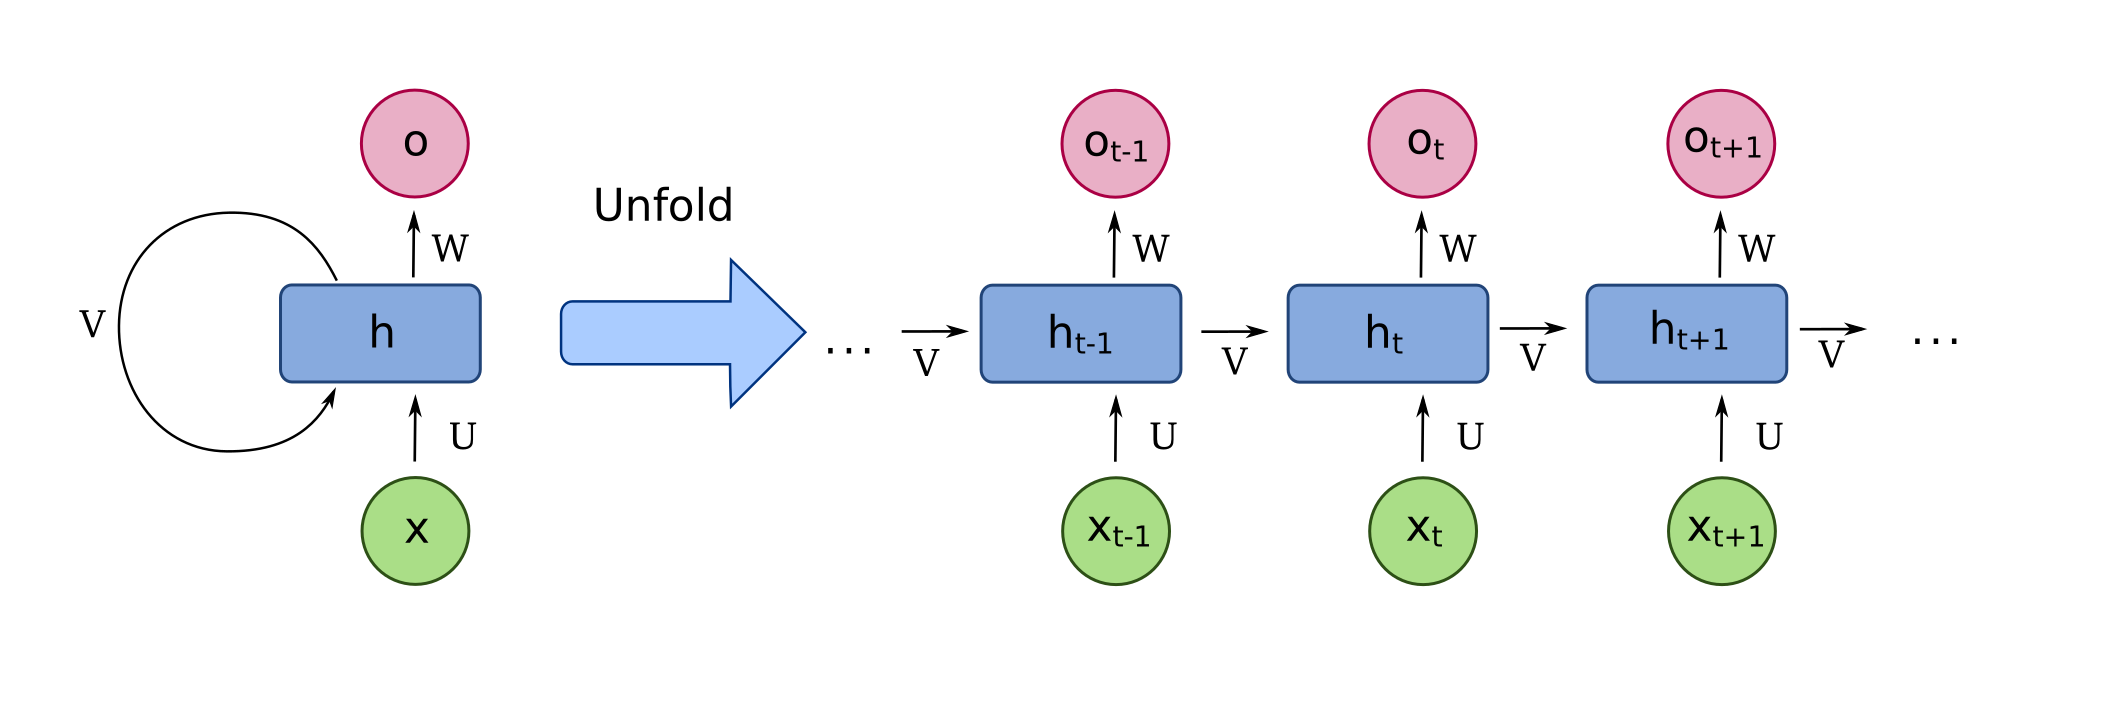
\includegraphics[width=15 cm]{images/rnn_unfold.png}
        \caption{Mô hình mạng neural hồi quy. \cite{rnn_unfold}}
        \label{fig:rnn_unfold}
    \end{figure}
    
    Dựa theo hình \ref{fig:rnn_unfold}, trong đó, $x_t$ và $o_t$ lần lượt là đầu vào và đầu ra tại thời điểm thứ $t$, $h_t$ là trạng thái ẩn tại thời điểm thứ $t$ và đóng vai trò là bộ nhớ của mạng. $h_t$ sẽ được tính dựa trên sự kết hợp giữa các trạng thái ẩn trước và đầu vào. Ta có thể viết:
    $$h_t = f(Ux_t + VS_{t-1}).$$
    
    Sau đó, $o_t$ sẽ được tính dựa theo $Wh_t$, với $(U, V, W)$ là ba tham số của mạng. Hai loại hàm truyền $f$ phổ biến nhất là hàm tanh hoặc hàm ReLU.
    
    Với khả năng “nhớ” được, mạng neural hồi quy được sử dụng để xử lý thông tin dạng chuỗi và các dữ liệu thời gian. Một số ứng dụng tiêu biểu là: mô hình ngôn ngữ và phát sinh văn bản, dịch máy (Machine Translation) và phát sinh mô tả cho ảnh (Generating Image Descriptions).
    
    \subsubsection{Hạn chế của RNN}
    Việc huấn luyện một RNN, cũng tương tự như mạng bình thường, sẽ sử dụng lan truyền ngược - Backpropagation như trên. Tuy nhiên, do bản chất có bộ nhớ của RNN, quá trình lan truyền ngược này sẽ được thực hiện qua từng thời điểm trong mạng. Quá trình này được gọi là \textit{lan truyền ngược liên hồi} (backpropagation through time).
    
    Mục tiêu là tính đạo hàm của lỗi với tham số $(U, V, W)$ tương ứng, sau đó, học các tham số này bằng cách sử dụng gradient descent. Ta có, ở từng trạng thái $h$, đạo hàm của hàm lỗi được khai triển như sau:
    $$\sum_t\dfrac{\partial e_t(\textbf{w})}{\partial\textbf{w}}\propto\sum_t\left(\prod_{i=k+1}\dfrac{\partial h_i}{\partial h_{i-1}}\right)\dfrac{\partial h_k}{\partial\textbf{w}}.$$
    
    Giả sử, trong trường hợp giá trị $\left\|\dfrac{\partial h_i}{\partial h_{i-1}}\right\|_2 < 1$, giá trị cập nhật sẽ bị giảm về gần 0 rất nhanh. Ví dụ, nếu lượng cập nhật chỉ là 0.01, nhưng qua 100 thời điểm, thì giá trị trên sẽ là $0.01^{100} \approx 0$. Mà khi đạo hàm bằng 0 thì có nghĩa là xảy ra hiện tượng bão hòa dẫn đến các nút phía trước cũng sẽ bị bão hoà theo. Vấn đề này không chỉ xảy ra với mạng RNN mà ngay cả mạng neural thường khá sâu cũng có hiện tượng này. Người ta gọi đây là hiện tượng \textbf{mất mát đạo hàm} (vanishing gradient).
    
    Một phương pháp phổ biến để giải quyết tình trạng mất mát đạo hàm là sử dụng kiến trúc mạng nhớ dài-ngắn hạn (Long Short-Term Memory (LSTM)). 
    
    \subsubsection{Long Short-Term Memory (LSTM)}
    \begin{figure}[htp]
        \centering
        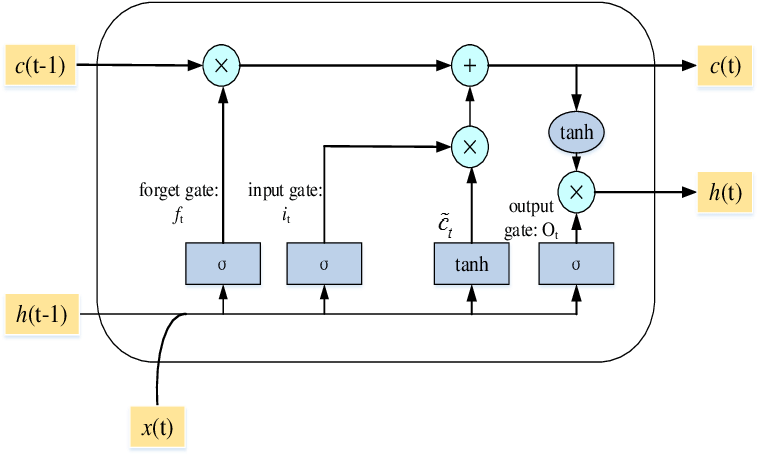
\includegraphics[width=14 cm]{images/lstm_struct.png}
        \caption{Cấu trúc của LSTM. \cite{lstm_struct}}
        \label{fig:lstm_struct}
    \end{figure}
    LSTM là một mô hình cải tiến của RNN và có cấu trúc tương tự nhưng khác ở cách tính toán đối với các trạng thái ẩn. Mấu chốt của khả năng “nhớ lâu” của LSTM là cấu trúc “trạng thái nhớ”. Ngoài ra, quá trình thêm hoặc loại bỏ thông tin sẽ dựa trên qui định của các cổng. Tóm lại, cốt lõi của mạng LSTM bao gồm trạng thái nhớ và các cổng.
    
    Các cổng của LSTM là một phương pháp định nghĩa thông tin băng qua và chúng được tạo bắng hàm sigmoid $\sigma$. Cụ thể, hàm sigmoid có giá trị thuộc khoảng (0, 1) mang ý nghĩa độ lớn thông tin được phép truyền qua tại mỗi lớp mạng. Nếu kết quả là 0,  điều này có nghĩa là không thông tin nào được phép đi qua, và ngươc lại, 1 nghĩa là toàn bộ thông tin được đi qua.
    
    Một mạng LSTM có 3 loại cổng, đều có đầu vào là trạng thái trước, đặt tên là $S \in \{h, c\}$, và đầu vào, nhân với trọng số tương ứng. Lưu ý, các cổng sẽ nhận một loại trọng sô khác nhau:
    \begin{itemize}
        \item \textbf{Cổng quên (Forget gate)} $f_t = \sigma(W_fS_{t-1} + W_fX_t)$.
        \item \textbf{Cổng vào (Input gate)} $i_t = \sigma(W_iS_{t-1} + W_iX_t)$
        \item \textbf{Cổng ra (Output gat)} $o_t = \sigma(W_oS_{t-1} + W_oX_t)$
    \end{itemize}
    
    Sau đó, trạng thái nhớ trung gian có thể được tính bằng hàm tanh qua công thức $\Tilde{C}_t = \text{tanh}(W_cS_{t-1} + W_cX_t)$. Từ đây, \textbf{trạng thái nhớ} sẽ nhận trạng thái trung gian và trạng thái nhớ trước, kết hợp với cổng vào và cổng quên như sau:
    \begin{equation} \label{lstm_cell_state_eqn}
        c_t = (i_t\times\Tilde{C}_t) + (f_t\times c_{t - 1}).
    \end{equation}
    
    Cuối cùng, trạng thái ẩn sẽ được tính bằng hàm tanh của trạng thái nhớ nhân với cổng ra:
    \begin{equation} \label{lstm_hidden_state_eqn}
        h_t = o_t\times\text{tanh}(c_t).
    \end{equation}
    
    Lưu ý, phép nhân trong công thức \ref{lstm_cell_state_eqn} và \ref{lstm_hidden_state_eqn} phụ thuộc vào $S$, tức là, các cổng sẽ thực hiện tính cho cả $h$ và $c$, sau đó, thực hiện phép nhân tương ứng cho mỗi loại trạng thái.

\section{Giới thiệu các bộ chuẩn hóa dữ liệu} \label{sec:basis-scaler}
\subsection {Chuẩn hóa dữ liệu với Min-Max Scaler}
\label{scaler:minmax}

Trong học máy, việc chuẩn hóa dữ liệu đầu vào giúp mô hình học hiệu quả hơn, đặc biệt với các mô hình nhạy cảm với thang đo (như KNN, SVM, hồi quy Logistic, mạng nơ-ron,...).

Một trong các phương pháp chuẩn hóa phổ biến là \textbf{Min-Max Scaling}, hay còn gọi là \textit{feature normalization}.

\textbf{Công thức Min-Max Scaling}

\[
x_i^{\text{scaled}} = \frac{x_i - x_{\min}}{x_{\max} - x_{\min}}
\]

Trong đó:
\begin{itemize}
    \item \( x_i \): giá trị gốc của đặc trưng.
    \item \( x_{\min} \): giá trị nhỏ nhất của đặc trưng trong tập dữ liệu.
    \item \( x_{\max} \): giá trị lớn nhất của đặc trưng.
    \item \( x_i^{\text{scaled}} \): giá trị sau khi chuẩn hóa.
\end{itemize}

\textbf{Ý nghĩa}

Min-Max Scaler biến đổi các đặc trưng về khoảng giá trị \([0, 1]\), giúp:

\begin{itemize}
    \item Tăng tốc độ hội tụ của thuật toán tối ưu.
    \item Tránh hiện tượng một vài đặc trưng chi phối quá trình học do thang đo lớn.
    \item Dữ liệu có cùng thang đo, phù hợp với các mô hình tính toán khoảng cách.
\end{itemize}

\textbf{Ví dụ}

Cho tập dữ liệu: \( x = [20, 40, 60, 80, 100] \)

\begin{itemize}
    \item \( x_{\min} = 20 \), \( x_{\max} = 100 \)
    \item \( x_3 = 60 \Rightarrow x_3^{\text{scaled}} = \frac{60 - 20}{100 - 20} = \frac{40}{80} = 0.5 \)
\end{itemize}

\textbf{Lưu ý}

\begin{itemize}
    \item Cần áp dụng giá trị \( x_{\min}, x_{\max} \) từ tập huấn luyện cho cả tập kiểm tra.
    \item Không nên dùng Min-Max Scaling nếu dữ liệu chứa nhiều ngoại lệ (nên dùng Robust Scaler).
\end{itemize}

\subsection{Chuẩn hóa dữ liệu với Standard Scaler}
\label{scaler:standard}

Trong học máy, việc chuẩn hóa dữ liệu giúp các mô hình hoạt động hiệu quả hơn, đặc biệt với các thuật toán nhạy cảm với độ lớn của đặc trưng như: hồi quy Logistic, KNN, SVM, mạng nơ-ron,...

Một kỹ thuật chuẩn hóa phổ biến là \textbf{Standard Scaler} – biến đổi dữ liệu sao cho có trung bình bằng 0 và độ lệch chuẩn bằng 1.

\textbf{Công thức chuẩn hóa Standard Scaler}

\[
x_i^{\text{scaled}} = \frac{x_i - \mu}{\sigma}
\]

Trong đó:
\begin{itemize}
    \item \( x_i \): giá trị gốc của đặc trưng.
    \item \( \mu \): trung bình (mean) của đặc trưng.
    \item \( \sigma \): độ lệch chuẩn (standard deviation).
    \item \( x_i^{\text{scaled}} \): giá trị sau khi chuẩn hóa.
\end{itemize}

\textbf{Ý nghĩa}

\begin{itemize}
    \item Dữ liệu sau chuẩn hóa có phân phối chuẩn hóa chuẩn: \( \mathcal{N}(0, 1) \).
    \item Trung bình bằng 0 và phương sai bằng 1 giúp mô hình học ổn định hơn.
\end{itemize}

\textbf{Ví dụ}

Cho tập dữ liệu: \( x = [10, 12, 14, 16, 18] \)

\begin{itemize}
    \item Trung bình \( \mu = 14 \), độ lệch chuẩn \( \sigma = \sqrt{\frac{(4^2 + 2^2 + 0^2 + 2^2 + 4^2)}{5}} = \sqrt{8} \approx 2.828 \)
    \item \( x_1^{\text{scaled}} = \frac{10 - 14}{\sigma} \approx \frac{-4}{2.828} \approx -1.414 \)
\end{itemize}

\textbf{Lưu ý}

\begin{itemize}
    \item Nên tính \( \mu \) và \( \sigma \) trên tập huấn luyện, rồi áp dụng lên cả tập kiểm tra.
    \item Phù hợp nếu dữ liệu có phân phối gần chuẩn.
    \item Không phù hợp khi có nhiều ngoại lệ → khi đó dùng RobustScaler.
\end{itemize}

\subsection{Chuẩn hóa dữ liệu với Robust Scaler}
\label{scaler:robust}

\textbf{Robust Scaler} là một kỹ thuật chuẩn hóa dữ liệu giúp giảm ảnh hưởng của các giá trị ngoại lệ (outliers). Khác với Min-Max Scaler (dựa trên max/min) hay Standard Scaler (dựa trên trung bình/độ lệch chuẩn), Robust Scaler sử dụng các số liệu thống kê mạnh như \textbf{trung vị} (median) và \textbf{IQR – khoảng tứ phân vị}.

\textbf{Công thức chuẩn hóa}

\[
x_i^{\text{scaled}} = \frac{x_i - \text{Median}(x)}{\text{IQR}(x)}
\]

Trong đó:
\begin{itemize}
    \item \( \text{Median}(x) \): trung vị của đặc trưng.
    \item \( \text{IQR}(x) = Q_3 - Q_1 \): khoảng tứ phân vị (Interquartile Range), với:
        \begin{itemize}
            \item \( Q_1 \): phân vị thứ 25\% (lower quartile)
            \item \( Q_3 \): phân vị thứ 75\% (upper quartile)
        \end{itemize}
    \item \( x_i^{\text{scaled}} \): giá trị sau chuẩn hóa.
\end{itemize}

\textbf{Ưu điểm}

\begin{itemize}
    \item Không bị ảnh hưởng mạnh bởi ngoại lệ.
    \item Giữ nguyên phân phối cơ bản của dữ liệu phần lớn.
    \item Phù hợp với các mô hình yêu cầu dữ liệu chuẩn hóa như KNN, SVM, Logistic Regression.
\end{itemize}

\textbf{Ví dụ}

Giả sử đặc trưng \( x = [10, 12, 14, 16, 100] \)

\begin{itemize}
    \item \( \text{Median}(x) = 14 \)
    \item \( Q_1 = 12, Q_3 = 16 \Rightarrow \text{IQR} = 4 \)
    \item \( x_5^{\text{scaled}} = \frac{100 - 14}{4} = 21.5 \)
    \item Trong khi Min-Max sẽ nén dữ liệu về [0,1], nhưng sẽ bị kéo lệch vì 100 là ngoại lệ.
\end{itemize}

\textbf{Lưu ý}

\begin{itemize}
    \item Nên tính Median và IQR từ tập huấn luyện và áp dụng cho tập kiểm tra.
    \item Không thích hợp nếu dữ liệu đã phân bố chuẩn và không có ngoại lệ → dùng StandardScaler.
\end{itemize}

\subsection{Chuẩn hóa dữ liệu với MaxAbsScaler}
\label{scaler:maxabs}

\textbf{MaxAbsScaler} là một kỹ thuật chuẩn hóa dữ liệu theo phương pháp co dãn tuyến tính (linear scaling), sử dụng giá trị tuyệt đối lớn nhất trong từng đặc trưng để đưa dữ liệu về khoảng \([-1, 1]\), mà vẫn giữ nguyên dấu gốc của dữ liệu.

\textbf{Công thức chuẩn hóa}

\[
x_i^{\text{scaled}} = \frac{x_i}{\max \left( |x| \right)}
\]

Trong đó:
\begin{itemize}
    \item \( x_i \): giá trị ban đầu của đặc trưng.
    \item \( \max(|x|) \): giá trị tuyệt đối lớn nhất trong đặc trưng đó.
    \item \( x_i^{\text{scaled}} \): giá trị sau chuẩn hóa, nằm trong khoảng \( [-1, 1] \).
\end{itemize}

\textbf{Đặc điểm}

\begin{itemize}
    \item Dữ liệu được chia cho giá trị tuyệt đối lớn nhất, nên không làm thay đổi sparsity (độ thưa).
    \item Giữ nguyên dấu ban đầu của dữ liệu.
    \item Thích hợp với dữ liệu có giá trị cả âm và dương, đặc biệt là dữ liệu sparse (rất nhiều giá trị 0).
\end{itemize}

\textbf{Ví dụ}

Cho đặc trưng \( x = [-3, -1, 0, 2, 4] \):

\[
\max(|x|) = 4, \quad x^{\text{scaled}} = \left[ \frac{-3}{4}, \frac{-1}{4}, 0, \frac{2}{4}, \frac{4}{4} \right] = [-0.75, -0.25, 0, 0.5, 1.0]
\]

\textbf{Lưu ý}

\begin{itemize}
    \item Phù hợp với dữ liệu sparse (tránh tạo thêm giá trị khác 0).
    \item Không xử lý outlier – giá trị cực trị vẫn ảnh hưởng đến việc scale.
    \item Không trung tâm hóa dữ liệu (không đưa trung bình về 0).
\end{itemize}

\subsection{Chuẩn hóa dữ liệu với Quantile Transformer}
\label{scaler:quantile}

\textbf{Quantile Transformer} là một phương pháp chuẩn hóa dữ liệu phi tuyến, chuyển đổi phân phối gốc của dữ liệu về một phân phối mục tiêu (thường là phân phối chuẩn hoặc phân phối đều) bằng cách sử dụng \textbf{phân vị (quantiles)}.

\textbf{Ý tưởng chính}

Quantile Transformer thực hiện hai bước:

\begin{enumerate}
    \item Ánh xạ mỗi giá trị dữ liệu sang giá trị phân vị tương ứng trong tập huấn luyện.
    \item Biến đổi các phân vị đó sang giá trị trong phân phối mục tiêu: \textit{uniform} hoặc \textit{normal}.
\end{enumerate}

\textbf{Biến đổi phân vị}

Giả sử dữ liệu ban đầu là \( x \in \mathbb{R} \), ta có:

\[
x_i^{\text{scaled}} = F_{\text{target}}^{-1}(F_{\text{empirical}}(x_i))
\]

Trong đó:
\begin{itemize}
    \item \( F_{\text{empirical}}(x_i) \): phân phối tích lũy thực nghiệm (ECDF) – giá trị phân vị của \( x_i \)
    \item \( F_{\text{target}}^{-1} \): hàm nghịch đảo của phân phối mục tiêu (chuẩn hoặc đều)
    \item \( x_i^{\text{scaled}} \): giá trị sau khi chuẩn hóa
\end{itemize}

\textbf{Phân phối đầu ra}

\begin{itemize}
    \item \textbf{Uniform} (phân phối đều): đưa dữ liệu về khoảng \([0, 1]\)
    \item \textbf{Normal} (phân phối chuẩn): đưa dữ liệu về phân phối chuẩn \( \mathcal{N}(0, 1) \)
\end{itemize}

\textbf{Ưu điểm}

\begin{itemize}
    \item Biến đổi phân phối lệch về phân phối chuẩn/đều → cải thiện hiệu suất mô hình.
    \item Giảm tác động của ngoại lệ (outliers).
    \item Phù hợp với các mô hình tuyến tính hoặc giả định phân phối chuẩn.
\end{itemize}

\textbf{Nhược điểm}

\begin{itemize}
    \item Là phép biến đổi phi tuyến → có thể làm mất quan hệ tuyến tính gốc.
    \item Dễ bị overfit nếu tập huấn luyện nhỏ.
\end{itemize}

\textbf{Ví dụ đơn giản}

Cho dữ liệu \( x = [10, 100, 1000] \)

\begin{itemize}
    \item \( 10 \rightarrow \text{quantile} = 0.0 \)
    \item \( 100 \rightarrow \text{quantile} = 0.5 \)
    \item \( 1000 \rightarrow \text{quantile} = 1.0 \)
    \item Nếu dùng phân phối chuẩn: giá trị tương ứng sẽ là \( [-\infty, 0, +\infty] \)
\end{itemize}


\section{Giới thiệu các chỉ số đánh giá hiệu suất mô hình}
\subsection {Accuracy (Độ chính xác)}
\label{eval:acc}
Accuracy là độ đo đơn giản nhất dùng để đánh giá hiệu suất của mô hình phân loại, được tính bằng tỷ lệ giữa số lượng dự đoán đúng và tổng số dự đoán:

\begin{equation}
\text{Accuracy} = \frac{TP + TN}{TP + TN + FP + FN}
\end{equation}

Ví dụ với bài toán phân loại \textit{Cat/Non-cat}, giả sử có 90 ảnh \textit{Cat} được phân loại đúng, 10 ảnh \textit{Cat} bị phân loại sai, 940 ảnh \textit{Non-cat} phân loại đúng và 60 ảnh \textit{Non-cat} bị phân loại sai. Khi đó:

\begin{equation}
\text{Accuracy} = \frac{90 + 940}{1000 + 100} = 93.6\%
\end{equation}

Tuy nhiên, Accuracy không phản ánh cụ thể mô hình xử lý tốt nhóm nào, dễ gây hiểu nhầm nếu dữ liệu mất cân bằng.

\subsection {F1-score}
\label{eval:f1}
Khi cả Precision và Recall đều quan trọng, ta sử dụng F1-score, là trung bình điều hòa của Precision và Recall:

\begin{equation}
\text{F1-score} = 2 \cdot \frac{\text{Precision} \cdot \text{Recall}}{\text{Precision} + \text{Recall}}
\end{equation}

F1-score giúp cân bằng giữa Precision và Recall, đặc biệt hữu ích khi dữ liệu bị mất cân bằng.

\subsection {Precision}
\label{eval:prec}
Precision đo lường tỷ lệ dự đoán dương tính đúng trong tất cả các dự đoán dương tính:

\begin{equation}
\text{Precision} = \frac{TP}{TP + FP}
\end{equation}

Áp dụng cho bài toán \textit{Cat/Non-cat}:

\begin{align*}
\text{Precision}_{\text{Cat}} &= \frac{90}{90 + 60} = 60\% \\
\text{Precision}_{\text{Non-cat}} &= \frac{940}{940 + 10} = 98.9\%
\end{align*}

Precision giúp đánh giá mô hình có dự đoán nhầm quá nhiều hay không trong nhóm dương tính.

\subsection {Recall}
\label{eval:prec}
Recall (Sensitivity, True Positive Rate) là tỷ lệ phát hiện đúng các mẫu dương tính thực sự:

\begin{equation}
\text{Recall} = \frac{TP}{TP + FN}
\end{equation}

Ví dụ:

\begin{align*}
\text{Recall}_{\text{Cat}} &= \frac{90}{90 + 10} = 90\% \\
\text{Recall}_{\text{Non-cat}} &= \frac{940}{940 + 60} = 94\%
\end{align*}

Recall cao thể hiện mô hình ít bỏ sót mẫu dương tính thực sự.

\subsection {ROC AUC}
\label{eval:rocauc}
\textbf{ROC Curve} (Receiver Operating Characteristic Curve) là biểu đồ thể hiện mối quan hệ giữa TPR và FPR:

\begin{align}
\text{TPR} &= \frac{TP}{TP + FN} \quad (\text{Recall}) \\
\text{FPR} &= \frac{FP}{FP + TN}
\end{align}

\textbf{AUC} (Area Under the Curve) là diện tích dưới đường cong ROC, biểu thị tổng quát khả năng phân loại của mô hình. AUC có giá trị từ 0 đến 1:
\begin{itemize}
    \item AUC gần 1: mô hình phân loại tốt.
    \item AUC gần 0.5: mô hình phân loại ngẫu nhiên.
\end{itemize}

Ví dụ: Với đầu ra xác suất $[0.45, 0.6, 0.7, 0.3]$, ta thay đổi ngưỡng để xác định nhãn phân loại. Khi vẽ TPR và FPR ứng với nhiều ngưỡng, ta có thể vẽ được ROC Curve. Diện tích dưới đường cong chính là AUC.

\textbf{Giải thích chi tiết các tham số}

Các độ đo như Accuracy, Precision, Recall, F1-score,... đều dựa trên \textbf{Ma trận nhầm lẫn (Confusion Matrix)}. Ma trận này được xây dựng dựa trên so sánh giữa nhãn dự đoán của mô hình và nhãn thực tế. Đối với bài toán phân loại nhị phân (binary classification), ma trận nhầm lẫn có 4 phần tử chính:

\begin{center}
\begin{tabular}{|c|c|c|}
\hline
 & \textbf{Dự đoán: Positive} & \textbf{Dự đoán: Negative} \\
\hline
\textbf{Thực tế: Positive} & TP (True Positive) & FN (False Negative) \\
\hline
\textbf{Thực tế: Negative} & FP (False Positive) & TN (True Negative) \\
\hline
\end{tabular}
\end{center}

\begin{itemize}
    \item \textbf{TP (True Positive)}: Số mẫu dương tính được mô hình dự đoán đúng là dương tính.
    \item \textbf{TN (True Negative)}: Số mẫu âm tính được mô hình dự đoán đúng là âm tính.
    \item \textbf{FP (False Positive)}: Số mẫu âm tính bị mô hình dự đoán nhầm là dương tính (hay còn gọi là lỗi loại I).
    \item \textbf{FN (False Negative)}: Số mẫu dương tính bị mô hình dự đoán nhầm là âm tính (hay còn gọi là lỗi loại II).
\end{itemize}


\subsection {Mean Squared Error (MAE)}
\label{eval:mse}

MSE (Mean Squared Error) là một trong những độ đo phổ biến nhất dùng để đánh giá hiệu suất của các mô hình hồi quy. Nó đo lường sai số trung bình bình phương giữa giá trị dự đoán và giá trị thực tế.

Giả sử với một bộ dữ liệu gồm $n$ mẫu, giá trị thực tế được ký hiệu là $y_i$, giá trị dự đoán là $\hat{y}_i$, thì MSE được tính theo công thức:

\begin{equation}
\text{MSE} = \frac{1}{n} \sum_{i=1}^{n} (y_i - \hat{y}_i)^2
\end{equation}

MSE phạt nặng các sai số lớn do sai số được bình phương. Do đó, MSE nhạy cảm với các điểm ngoại lai (\textit{outliers}).

\vspace{0.3cm}
\noindent\textbf{Ví dụ:} Trong bài toán dự đoán giá nhà, $y_i$ là giá trị thực tế của căn nhà thứ $i$, và $\hat{y}_i$ là giá trị dự đoán. MSE sẽ đo lường khoảng cách trung bình bình phương giữa các giá trị này.


\subsection {Mean Absolute Error (MAE)}
\label{eval:mae}
MAE (Mean Absolute Error) là một độ đo khác, đánh giá sai số trung bình tuyệt đối giữa giá trị thực tế và giá trị dự đoán:

\begin{equation}
\text{MAE} = \frac{1}{n} \sum_{i=1}^{n} |y_i - \hat{y}_i|
\end{equation}

Không giống như MSE, MAE sử dụng trị tuyệt đối thay vì bình phương, do đó nó ít bị ảnh hưởng bởi các điểm ngoại lai. MAE được coi là một metric \textit{mạnh hơn} khi mô hình cần khả năng chống chịu với dữ liệu nhiễu.

\vspace{0.3cm}
\noindent\textbf{So sánh MSE và MAE:}
\begin{itemize}
    \item \textbf{MSE} nhấn mạnh các lỗi lớn (do bình phương sai số), phù hợp khi muốn phạt mạnh các dự đoán sai nhiều.
    \item \textbf{MAE} phản ánh mức sai lệch trung bình thực sự, bền vững hơn với các ngoại lai.
\end{itemize}

\subsection {Root Mean Squared Error (RMSE)}
\label{eval:rmse}
RMSE (Root Mean Squared Error) là một metric đánh giá độ lệch giữa giá trị dự đoán và giá trị thực tế trong các bài toán hồi quy. RMSE chính là căn bậc hai của MSE (Mean Squared Error), do đó vẫn giữ đặc tính "phạt nặng" các sai số lớn, nhưng giá trị của nó có cùng đơn vị với biến đầu ra.

\textbf{Công thức tính RMSE}

Giả sử có $n$ mẫu dữ liệu, $y_i$ là giá trị thực tế, và $\hat{y}_i$ là giá trị dự đoán của mô hình. Khi đó, RMSE được tính như sau:

\begin{equation}
\text{RMSE} = \sqrt{ \frac{1}{n} \sum_{i=1}^{n} (y_i - \hat{y}_i)^2 }
\end{equation}

\textbf{Ý nghĩa}

\begin{itemize}
    \item RMSE biểu thị độ lệch chuẩn của sai số dự đoán.
    \item Đơn vị của RMSE giống với đơn vị của biến đầu ra, giúp dễ diễn giải trong thực tế.
    \item RMSE nhạy cảm với các điểm ngoại lai (outliers) hơn so với MAE, do bình phương sai số.
\end{itemize}

\subsubsection*{So sánh RMSE và MSE}

\begin{itemize}
    \item \textbf{MSE}: thường được dùng cho mục đích tối ưu trong huấn luyện mô hình (ví dụ trong đạo hàm của hàm mất mát).
    \item \textbf{RMSE}: thường được dùng để báo cáo kết quả mô hình vì đơn vị dễ hiểu hơn.
\end{itemize}

\textbf{Ví dụ}

Nếu mô hình dự đoán giá nhà, trong đó giá trị thực tế và dự đoán tính bằng triệu đồng, thì RMSE = 50 nghĩa là sai số trung bình của mô hình là khoảng \textbf{50 triệu đồng}.


\subsection {Mean Absolute Percentage Error (MAPE)}
\label{eval:mape}
MAPE (Mean Absolute Percentage Error) là một độ đo thường được sử dụng trong các bài toán hồi quy để đánh giá sai số trung bình phần trăm giữa giá trị dự đoán và giá trị thực tế.

\textbf{Công thức tính}

Giả sử ta có $n$ mẫu dữ liệu, với $y_i$ là giá trị thực tế và $\hat{y}_i$ là giá trị dự đoán tương ứng. Công thức tính MAPE như sau:

\begin{equation}
\text{MAPE} = \frac{100\%}{n} \sum_{i=1}^{n} \left| \frac{y_i - \hat{y}_i}{y_i} \right|
\end{equation}

\textbf{Ý nghĩa}

\begin{itemize}
    \item MAPE biểu thị sai số trung bình theo phần trăm so với giá trị thực tế.
    \item MAPE dễ diễn giải và thường được sử dụng trong các bài toán dự báo thời gian (\textit{forecasting}).
    \item Ví dụ: MAPE = 8.5\% nghĩa là trung bình mô hình dự đoán sai lệch 8.5\% so với giá trị thực tế.
\end{itemize}

\textbf{Ưu và nhược điểm}

\begin{itemize}
    \item \textbf{Ưu điểm:}
        \begin{itemize}
            \item Diễn giải trực quan dưới dạng phần trăm.
            \item Không phụ thuộc vào đơn vị đo.
        \end{itemize}
    \item \textbf{Nhược điểm:}
        \begin{itemize}
            \item Không xác định được nếu có $y_i = 0$ (chia cho 0).
            \item Nhạy cảm với các giá trị thực nhỏ, dễ làm tăng sai số phần trăm.
        \end{itemize}
\end{itemize}

\textbf{Lưu ý khi sử dụng}

MAPE không phù hợp nếu tập dữ liệu chứa các giá trị thực tế bằng 0 hoặc gần 0. Trong các trường hợp này, nên dùng SMAPE (Symmetric MAPE) hoặc các metric khác như MAE, RMSE.

\subsection{Adjusted Rand Index (ARI)}
\textbf{Khái niệm}

Adjusted Rand Index (ARI) là một độ đo thống kê dùng để đánh giá mức độ tương đồng giữa hai tập phân cụm: một là kết quả phân cụm của mô hình, và một là nhãn thực (ground truth), nếu có. ARI điều chỉnh theo sự ngẫu nhiên, giúp khắc phục nhược điểm của chỉ số Rand gốc (Rand Index - RI), vốn có thể cho giá trị cao ngay cả khi hai phân cụm gần như ngẫu nhiên.

Chỉ số ARI được sử dụng phổ biến trong các bài toán phân cụm khi muốn so sánh mức độ chính xác của mô hình phân cụm không giám sát với phân nhóm thực tế.

\textbf{Công thức tính ARI}

Giả sử ta có:
\begin{itemize}
    \item $n$: Tổng số điểm dữ liệu.
    \item $X = \{X_1, X_2, \ldots, X_r\}$: Tập phân cụm thực tế gồm $r$ cụm.
    \item $Y = \{Y_1, Y_2, \ldots, Y_s\}$: Tập phân cụm dự đoán gồm $s$ cụm.
\end{itemize}

Gọi $n_{ij}$ là số phần tử nằm đồng thời trong cụm $X_i$ và $Y_j$.

Gọi:
\begin{align*}
a_i &= \sum_{j} n_{ij} \quad \text{(tổng số điểm trong cụm thực tế $X_i$)} \\
b_j &= \sum_{i} n_{ij} \quad \text{(tổng số điểm trong cụm dự đoán $Y_j$)}
\end{align*}

Khi đó, công thức ARI được tính như sau:

\begin{equation}
\text{ARI} = \frac{
    \sum_{ij} \binom{n_{ij}}{2}
    - \left[ \sum_i \binom{a_i}{2} \sum_j \binom{b_j}{2} \middle/ \binom{n}{2} \right]
}{
    \frac{1}{2} \left[ \sum_i \binom{a_i}{2} + \sum_j \binom{b_j}{2} \right]
    - \left[ \sum_i \binom{a_i}{2} \sum_j \binom{b_j}{2} \middle/ \binom{n}{2} \right]
}
\end{equation}

\textbf{Giải thích ý nghĩa}

\begin{itemize}
    \item ARI có giá trị nằm trong khoảng $[-1, 1]$.
    \item ARI = 1 khi hai phân cụm hoàn toàn khớp nhau.
    \item ARI $\approx$ 0 khi phân cụm gần như ngẫu nhiên.
    \item ARI < 0 có thể xảy ra nếu phân cụm kém hơn cả ngẫu nhiên.
\end{itemize}

\textbf{Ví dụ sử dụng}

Chẳng hạn trong bài toán phân cụm ảnh khuôn mặt hoặc nhóm khách hàng, ARI cho phép đánh giá mô hình phân cụm khi có nhãn thật để so sánh. Đây là công cụ hữu ích khi so sánh các thuật toán phân cụm như K-Means, DBSCAN, Agglomerative Clustering, v.v.

\chapter{Cơ sở lý thuyết} \label{chapt:basis}

\startcontents[chapters]

\section{Giới thiệu các thông số thống kê} \label{sec:basis-tstk}
\subsection {Mean (Trung bình)}
\label{stat:mean}
Mean (trung bình số học) là giá trị đại diện cho mức trung bình của một tập hợp số liệu. Đây là một trong những chỉ số trung tâm phổ biến nhất trong thống kê.

\begin{itemize}
    \item Trung bình cộng được tính theo công thức:
    \begin{equation}
        \label{eq:Mean}
        \bar{x} = \frac{1}{n} \sum_{i=1}^{n} x_i
    \end{equation}
\end{itemize}

Trong đó:
\begin{itemize}[noitemsep, topsep=0pt]
    \item $n$: Số lượng phần tử trong tập dữ liệu
    \item $x_i$: Giá trị của phần tử thứ $i$
\end{itemize}

Ví dụ:
\vspace{0.5em}
Cho tập dữ liệu: \fbox{3}, \fbox{5}, \fbox{7}, \fbox{10}
\[
    \bar{x} = \frac{3 + 5 + 7 + 10}{4} = \frac{25}{4} = 6.25
\]

\subsection {Median (Trung vị)}
\label{stat:med}
Median (hay còn gọi là trung vị) là giá trị nằm ở giữa của một tập hợp dữ liệu đã được sắp xếp theo thứ tự tăng dần hoặc giảm dần. Nó chia tập dữ liệu thành hai nửa bằng nhau, với một nửa các giá trị nhỏ hơn hoặc bằng trung vị và một nửa các giá trị lớn hơn hoặc bằng trung vị. 

Với một dãy số đã được sắp xếp tăng dần, ký hiệu \( x_{(1)}, x_{(2)}, \ldots, x_{(n)} \), trung vị được tính như sau:

\textbf{Trường hợp 1:} Nếu \( n \) là số lẻ
\begin{equation}
\label{eq:median_1}
\text{Median} = x_{\left( \frac{n+1}{2} \right)}
\end{equation}

\textbf{Trường hợp 2:} Nếu \( n \) là số chẵn
\begin{equation}
\label{eq:median_0}
\text{Median} = \frac{1}{2} \left( x_{\left( \frac{n}{2} \right)} + x_{\left( \frac{n}{2} + 1 \right)} \right)
\end{equation}

Ví dụ:
Nếu bạn có một tập dữ liệu như sau: 2, 3, 5, 7, 9, thì trung vị là 5, vì nó nằm ở giữa và có hai giá trị nhỏ hơn (2, 3) và hai giá trị lớn hơn (7, 9).

Nếu tập dữ liệu có số lượng giá trị chẵn, trung vị là trung bình cộng của hai giá trị ở giữa sau khi đã sắp xếp. 

Ví dụ, nếu tập dữ liệu là 2, 3, 5, 7, thì trung vị là $\frac{3 + 5}{2}$ = 4.

Khác biệt giữa trung vị và trung bình cộng:
Trung bình cộng (mean) là tổng của tất cả các giá trị trong tập dữ liệu chia cho số lượng giá trị, còn trung vị là giá trị ở giữa.

\textbf{Ưu điểm của Trung vị}
\begin{itemize}[noitemsep, topsep=0pt]
    \item \textbf{Ít bị ảnh hưởng bởi giá trị ngoại lệ (outliers):} Khác với trung bình cộng, trung vị không bị kéo lệch bởi các giá trị quá lớn hoặc quá nhỏ trong tập dữ liệu.
    \item \textbf{Phù hợp với phân bố không chuẩn:} Trung vị là đại lượng thích hợp để mô tả xu hướng trung tâm của các tập dữ liệu có phân bố lệch hoặc không đối xứng.
    \item \textbf{Đơn giản và dễ tính:} Việc xác định trung vị chỉ cần sắp xếp dữ liệu theo thứ tự và chọn giá trị giữa, nên không yêu cầu các phép tính phức tạp.
\end{itemize}

\textbf{Ứng dụng của Trung vị}
\begin{itemize}[noitemsep, topsep=0pt]
    \item \textbf{Trong thống kê mô tả:} Được sử dụng để mô tả xu hướng trung tâm trong các báo cáo thống kê, đặc biệt là khi dữ liệu không tuân theo phân phối chuẩn.
    \item \textbf{Trong lĩnh vực tài chính:} Trung vị được dùng để tính toán mức lợi nhuận điển hình, giá trị tài sản đầu tư, hoặc thu nhập hộ gia đình để tránh bị ảnh hưởng bởi các giá trị bất thường.
    \item \textbf{Trong y học:} Thường được sử dụng để mô tả các chỉ số sinh học như huyết áp, cholesterol... giúp phản ánh tình trạng sức khỏe điển hình trong dân số mà không bị ảnh hưởng bởi các ca bệnh hiếm.
    \item \textbf{Trong khoa học dữ liệu và máy học:} Trung vị được dùng để xử lý dữ liệu có phân phối lệch, phát hiện điểm bất thường, hoặc phân chia tập dữ liệu thành các phần có kích thước và đặc tính tương tự nhau (như chia thành tứ phân vị).
\end{itemize}

\subsection {Mode (Giá trị xuất hiện nhiều nhất)}
\label{stat:mode}

Mode  là giá trị xuất hiện nhiều nhất trong một tập hợp dữ liệu.
Nó là một trong ba đại lượng đo xu hướng trung tâm, cùng với Trung bình (Mean) và Trung vị (Median).

\begin{itemize}
    \item Mode được tính theo công thức:
    \begin{equation}
        \label{eq:Mode}
        \text{Mode} = \arg\max_{x_i} \left( \text{Frequency}(x_i) \right)
    \end{equation}
\end{itemize}

\begin{itemize}[noitemsep, topsep=0pt]
    \item Trong thống kê, Mode là giá trị được quan sát thấy tần suất xuất hiện nhiều nhất trong một tập hợp dữ liệu.

    \item Đối với phân phối chuẩn, Mode có cùng giá trị với giá trị trung bình và trung vị.

    \item Trong nhiều trường hợp, giá trị của Mode sẽ khác với giá trị trung bình. 
\end{itemize}

\textbf{Ưu điểm của Mode}
\begin{itemize}[noitemsep, topsep=0pt]
    \item Dễ hiểu và dễ tính toán.

    \item Không bị ảnh hưởng bởi các giá trị ngoại lai.

    \item Dễ dàng xác định trong các dữ liệu chưa được gộp và phân phối có tần số rời rạc.

    \item Hữu ích cho dữ liệu định tính.

    \item Có thể tính toán với bảng tần số không giới hạn.

    \item Có thể được xác định bằng hình ảnh.
\end{itemize}

\textbf{Nhược điểm của Mode}
\begin{itemize}[noitemsep, topsep=0pt]
    \item Không được định nghĩa rõ ràng.

    \item Không tạo thành dựa trên tất cả các giá trị trong tập dữ liệu.

    \item Chỉ ổn định cho số lượng giá trị nhiều và sẽ không được xác định rõ ràng nếu dữ liệu chỉ có một số lượng nhỏ các giá trị.

    \item Không có khả năng sử dụng tính toán thêm.

    \item Đôi khi dữ liệu có một hoặc nhiều Mode hoặc không có Mode nào cả.
\end{itemize}

\subsection {Percentile (Phân vị)}
\label{stat:percentile}

Phân vị thứ \( P \) là giá trị chia tập dữ liệu đã được sắp xếp thành 100 phần bằng nhau, sao cho \( P\% \) các quan sát có giá trị nhỏ hơn hoặc bằng giá trị này.

\textbf{Công thức tính vị trí phân vị}

Vị trí lý thuyết của phân vị thứ \( P \) trong dãy dữ liệu được sắp xếp tăng dần được xác định bằng công thức:

\begin{equation}
    L_P = \frac{P}{100}(n + 1)
    \label{eq:percentile-position}
\end{equation}

\noindent
Trong đó:

\begin{itemize}
    \item \( L_P \): Vị trí lý thuyết của phân vị thứ \( P \) trong tập dữ liệu đã được sắp xếp (có thể là số thập phân).
    \item \( P \): Giá trị phân vị cần tính, thuộc khoảng từ \( 0 \) đến \( 100 \).
    \item \( n \): Tổng số phần tử trong tập dữ liệu.
    \item \( \frac{P}{100} \): Tỷ lệ phần trăm tương ứng với phân vị thứ \( P \).
    \item \( n + 1 \): Hệ số điều chỉnh để tăng độ chính xác khi nội suy giữa các phần tử.
\end{itemize}

\textbf{Trường hợp nội suy}

Nếu \( L_P \) không phải là số nguyên, ta thực hiện nội suy tuyến tính giữa hai phần tử gần nhất trong tập dữ liệu đã sắp xếp.

Giả sử \( L_P = k + d \), trong đó \( k \in \mathbb{Z} \), \( 0 < d < 1 \), thì:

\begin{equation}
    \label{eq:percentile-position-2}
    \text{Percentile}_P = x_k + d \cdot (x_{k+1} - x_k)
\end{equation}

\noindent
Với:
\begin{itemize}
    \item \( x_k \): Phần tử ở vị trí thứ \( k \),
    \item \( x_{k+1} \): Phần tử kế tiếp sau \( x_k \),
    \item \( d \): Phần thập phân của \( L_P \).
\end{itemize}

\textbf{Ví dụ minh họa}

Giả sử tập dữ liệu đã được sắp xếp như sau:

\[
    2,\ 4,\ 6,\ 8,\ 10,\ 12,\ 14,\ 16,\ 18,\ 20
\]

\noindent
Với \( n = 10 \), ta tính phân vị thứ 25:

\[
    L_{25} = \frac{25}{100}(10 + 1) = 2.75
\]

Nội suy giữa giá trị ở vị trí 2 và 3:

\[
    \text{Percentile}_{25} = 4 + 0.75 \cdot (6 - 4) = 5.5
\]

\textbf{Ứng dụng của phân vị}

\begin{itemize}
    \item Xếp hạng học sinh theo điểm số.
    \item Đánh giá chỉ số cơ thể trong y tế (BMI, chiều cao...).
    \item Phân tích dữ liệu để phát hiện ngoại lệ.
    \item Trực quan hóa phân bố dữ liệu qua biểu đồ hộp (boxplot) với các tứ phân vị (Q1, Q2, Q3).
\end{itemize}

\subsection {Max and Min (Giá trị lớn nhất và nhỏ nhất)}
\label{stat:minmax}

Trong thống kê mô tả, hai giá trị quan trọng giúp xác định độ bao phủ của dữ liệu là giá trị lớn nhất và giá trị nhỏ nhất.

\textbf{Định nghĩa}

\begin{itemize}
    \item \textbf{Giá trị lớn nhất (Maximum - Max):} là phần tử có giá trị cao nhất trong tập dữ liệu.
    \item \textbf{Giá trị nhỏ nhất (Minimum - Min):} là phần tử có giá trị thấp nhất trong tập dữ liệu.
\end{itemize}

\textbf{Ký hiệu và công thức}

Cho tập dữ liệu gồm \( n \) phần tử: \( \{x_1, x_2, \ldots, x_n\} \), ta có:

\begin{itemize}
    \item \textbf{Giá trị lớn nhất (Max):}
    \[
        \max(x_i) = \max \{ x_1, x_2, \ldots, x_n \}
    \]
    
    \item \textbf{Giá trị nhỏ nhất (Min):}
    \[
        \min(x_i) = \min \{ x_1, x_2, \ldots, x_n \}
    \]
\end{itemize}

\textbf{Ví dụ minh họa}

Cho tập dữ liệu sau:

\[
7,\ 12,\ 5,\ 9,\ 14,\ 6
\]

\noindent Ta có:
\begin{align*}
\max(x_i) &= 14 \\
\min(x_i) &= 5
\end{align*}

\textbf{Ứng dụng trong thống kê và học máy}

\begin{itemize}
    \item \textbf{Tính phạm vi (Range):}
    \[
        \text{Range} = \max(x_i) - \min(x_i)
    \]

    \item \textbf{Chuẩn hóa dữ liệu (Min-Max normalization):}
    \[
        x' = \frac{x - \min(x)}{\max(x) - \min(x)}
    \]
    Phương pháp này giúp đưa dữ liệu về khoảng giá trị \([0, 1]\), thường được sử dụng trong học máy để cải thiện hiệu suất huấn luyện mô hình.

    \item \textbf{Phát hiện giá trị ngoại lệ (Outliers):}  
    Các giá trị quá xa so với min hoặc max có thể bị xem là bất thường nếu kết hợp với các phân vị (Q1, Q3) và khoảng tứ phân vị (IQR).
\end{itemize}


\subsection {Range (Khoảng biến thiên)}
\label{stat:range}

Phạm vi là một trong những thước đo đơn giản nhất của độ phân tán trong thống kê mô tả. Nó được tính bằng hiệu số giữa giá trị lớn nhất và giá trị nhỏ nhất trong tập dữ liệu.

\textbf{Công thức tính}

\begin{equation}
    \text{Range} = \max(x_i) - \min(x_i)
    \tag{2.4}
\end{equation}

\noindent
Trong đó:
\begin{itemize}
    \item \( \max(x_i) \): Giá trị lớn nhất trong tập dữ liệu \( \{x_1, x_2, \ldots, x_n\} \).
    \item \( \min(x_i) \): Giá trị nhỏ nhất trong tập dữ liệu.
    \item \( \text{Range} \): Phạm vi của dữ liệu, thể hiện độ trải rộng giữa hai giá trị cực trị.
\end{itemize}

\textbf{Đặc điểm}
\begin{itemize}
    \item Phạm vi rất dễ tính toán và giúp hình dung nhanh độ biến thiên của dữ liệu.
    \item Tuy nhiên, phạm vi "rất nhạy cảm với các giá trị ngoại lệ (outliers)", vì nó chỉ xét đến hai giá trị cực trị.
    \item Phù hợp sử dụng trong những trường hợp dữ liệu không có ngoại lệ rõ rệt hoặc cần ước lượng nhanh.
\end{itemize}

\textbf{Ví dụ minh họa}

Cho tập dữ liệu:

\[
    4,\ 7,\ 9,\ 10,\ 15
\]

\noindent
Ta có:

\[
    \max(x_i) = 15,\quad \min(x_i) = 4
\]

\[
    \Rightarrow \text{Range} = 15 - 4 = 11
\]


\subsection {Variance (Phương sai)}
\label{stat:var}

Phương sai là một đại lượng quan trọng dùng để đo mức độ phân tán (biến thiên) của dữ liệu so với giá trị trung bình. Nó cho biết các quan sát trong tập dữ liệu cách xa trung bình cộng bao nhiêu, tính theo bình phương.

\textbf{Ký hiệu và công thức}

Cho một tập dữ liệu \( \{x_1, x_2, \ldots, x_n\} \), với trung bình cộng là \( \bar{x} \), ta có:

\begin{itemize}
    \item \textbf{Phương sai mẫu (Sample variance)} được tính theo công thức:
    \begin{equation}
        s^2 = \frac{1}{n - 1} \sum_{i=1}^{n} (x_i - \bar{x})^2
        \label{eq:sample-variance}
    \end{equation}

    \item \textbf{Phương sai tổng thể (Population variance)}:
    \begin{equation}
        \sigma^2 = \frac{1}{n} \sum_{i=1}^{n} (x_i - \mu)^2
        \label{eq:population-variance}
    \end{equation}
\end{itemize}

Trong đó:
\begin{itemize}
    \item \( s^2 \): phương sai mẫu.
    \item \( \sigma^2 \): phương sai tổng thể.
    \item \( n \): số phần tử trong mẫu hoặc tổng thể.
    \item \( x_i \): giá trị quan sát thứ \( i \).
    \item \( \bar{x} \): trung bình mẫu.
    \item \( \mu \): trung bình tổng thể (nếu biết).
\end{itemize}

\textbf{Giải thích ý nghĩa}

Phương sai đo lường trung bình bình phương khoảng cách từ mỗi điểm dữ liệu đến trung bình. Giá trị phương sai càng lớn cho thấy dữ liệu phân tán rộng, phương sai càng nhỏ cho thấy dữ liệu tập trung gần trung bình.

\textbf{Ví dụ minh họa}

Cho tập dữ liệu:

\[
x = \{ 2,\ 4,\ 6,\ 8,\ 10 \}
\]

Tính trung bình:

\[
\bar{x} = \frac{2 + 4 + 6 + 8 + 10}{5} = 6
\]

Tính phương sai mẫu:

\[
s^2 = \frac{1}{5 - 1} \left[ (2 - 6)^2 + (4 - 6)^2 + (6 - 6)^2 + (8 - 6)^2 + (10 - 6)^2 \right]
= \frac{1}{4} (16 + 4 + 0 + 4 + 16) = \frac{40}{4} = 10
\]

\textbf{Ứng dụng}

\begin{itemize}
    \item Đo lường độ biến thiên trong dữ liệu.
    \item So sánh mức độ rủi ro trong tài chính (phân tán lợi nhuận).
    \item Là thành phần cơ bản để tính độ lệch chuẩn, hệ số tương quan, kiểm định giả thuyết.
    \item Dùng trong nhiều mô hình thống kê và học máy (hồi quy tuyến tính, PCA, v.v.).
\end{itemize}

\subsection {Standard Deviation (Độ lệch chuẩn)}
\label{stat:sd}

Độ lệch chuẩn là một thước đo thống kê phổ biến nhằm xác định mức độ phân tán của dữ liệu quanh giá trị trung bình. Nó là căn bậc hai của phương sai, giúp đưa đơn vị đo về cùng đơn vị với dữ liệu gốc, từ đó dễ diễn giải hơn.

\textbf{Công thức}

\begin{itemize}
    \item \textbf{Độ lệch chuẩn mẫu (Sample standard deviation)}:
    \begin{equation}
        s = \sqrt{\frac{1}{n - 1} \sum_{i=1}^{n} (x_i - \bar{x})^2}
        \label{eq:sample-sd}
    \end{equation}

    \item \textbf{Độ lệch chuẩn tổng thể (Population standard deviation)}:
    \begin{equation}
        \sigma = \sqrt{\frac{1}{n} \sum_{i=1}^{n} (x_i - \mu)^2}
        \label{eq:population-sd}
    \end{equation}
\end{itemize}

\noindent
Trong đó:
\begin{itemize}
    \item \( s \): Độ lệch chuẩn mẫu.
    \item \( \sigma \): Độ lệch chuẩn tổng thể.
    \item \( n \): Số phần tử trong mẫu hoặc tổng thể.
    \item \( x_i \): Giá trị quan sát thứ \( i \).
    \item \( \bar{x} \): Trung bình mẫu.
    \item \( \mu \): Trung bình tổng thể.
\end{itemize}

\textbf{Ý nghĩa}

Độ lệch chuẩn cho biết mức độ phân tán trung bình của các điểm dữ liệu so với trung bình cộng:

\begin{itemize}
    \item Độ lệch chuẩn \textbf{càng nhỏ} → dữ liệu \textbf{tập trung quanh trung bình}.
    \item Độ lệch chuẩn \textbf{càng lớn} → dữ liệu \textbf{phân tán rộng hơn}.
\end{itemize}

\textbf{Ví dụ minh họa}

Cho tập dữ liệu:

\[
x = \{ 2,\ 4,\ 6,\ 8,\ 10 \}
\]

Trung bình:

\[
\bar{x} = \frac{2 + 4 + 6 + 8 + 10}{5} = 6
\]

Tính độ lệch chuẩn mẫu:

\[
s = \sqrt{\frac{1}{4} \left[ (2 - 6)^2 + (4 - 6)^2 + (6 - 6)^2 + (8 - 6)^2 + (10 - 6)^2 \right]} = \sqrt{\frac{40}{4}} = \sqrt{10} \approx 3.16
\]

\textbf{Ứng dụng}

\begin{itemize}
    \item Được sử dụng rộng rãi trong thống kê mô tả để đo lường sự biến động.
    \item Là cơ sở cho nhiều phương pháp kiểm định giả thuyết (t-test, ANOVA...).
    \item Giúp đánh giá độ rủi ro trong tài chính, ví dụ như độ biến động của giá cổ phiếu.
    \item Được sử dụng trong học máy và khai phá dữ liệu để chuẩn hóa dữ liệu.
\end{itemize}

\subsection{Coefficient of Variation - CV (Hệ số biến thiên)}
\label{stat:coef}

Hệ số biến thiên là một chỉ số thống kê đo lường mức độ phân tán tương đối của dữ liệu so với trung bình cộng. Nó biểu thị độ lệch chuẩn dưới dạng phần trăm của giá trị trung bình.

\textbf{Công thức}

\begin{itemize}
    \item \textbf{Hệ số biến thiên của mẫu:}
    \begin{equation}
        CV = \frac{s}{\bar{x}} \times 100\%
        \label{eq:cv-sample}
    \end{equation}
    
    \item \textbf{Hệ số biến thiên của tổng thể:}
    \begin{equation}
        CV = \frac{\sigma}{\mu} \times 100\%
        \label{eq:cv-population}
    \end{equation}
\end{itemize}

Trong đó:
\begin{itemize}
    \item \( CV \): Hệ số biến thiên (thường biểu thị bằng phần trăm).
    \item \( s \): Độ lệch chuẩn mẫu.
    \item \( \bar{x} \): Trung bình mẫu.
    \item \( \sigma \): Độ lệch chuẩn tổng thể.
    \item \( \mu \): Trung bình tổng thể.
\end{itemize}

\textbf{Ý nghĩa}

\begin{itemize}
    \item CV đo lường mức độ biến động của dữ liệu **tương đối** so với trung bình.
    \item Hữu ích khi so sánh độ phân tán của các tập dữ liệu có đơn vị đo hoặc giá trị trung bình khác nhau.
    \item CV càng cao → dữ liệu biến động càng lớn.
    \item CV càng thấp → dữ liệu ổn định và tập trung hơn quanh trung bình.
\end{itemize}

\textbf{Ví dụ minh họa}

Cho tập dữ liệu sau:

\[
x = \{ 2,\ 4,\ 6,\ 8,\ 10 \}
\]

Ta đã biết:
\begin{align*}
\bar{x} &= 6 \\
s &= \sqrt{10} \approx 3.16
\end{align*}

Khi đó, hệ số biến thiên:

\[
CV = \frac{3.16}{6} \times 100\% \approx 52.67\%
\]

\textbf{Ứng dụng}

\begin{itemize}
    \item So sánh độ biến động của các chỉ số kinh tế, tài chính, năng suất sản xuất giữa các nhóm khác nhau.
    \item Đánh giá độ ổn định của dữ liệu trong nghiên cứu thí nghiệm, kiểm tra chất lượng, phân tích định lượng.
    \item Trong tài chính, CV được sử dụng để đánh giá rủi ro tương đối của các khoản đầu tư.
\end{itemize}

\subsection {Interquartile Range – IQR (Khoảng tứ phân vị)}
\label{stat:iqr}

Khoảng tứ phân vị (IQR – Interquartile Range) là một thước đo thống kê thể hiện phạm vi phân bố của nhóm dữ liệu trung bình, bằng hiệu số giữa tứ phân vị thứ ba (\(Q_3\)) và tứ phân vị thứ nhất (\(Q_1\)).

\textbf{Công thức tính IQR}

\begin{equation}
    \text{IQR} = Q_3 - Q_1
    \label{eq:iqr}
\end{equation}

\noindent Trong đó:
\begin{itemize}
    \item \( Q_1 \): Tứ phân vị thứ nhất (25\% số quan sát nhỏ hơn hoặc bằng).
    \item \( Q_3 \): Tứ phân vị thứ ba (75\% số quan sát nhỏ hơn hoặc bằng).
    \item \( \text{IQR} \): Khoảng tứ phân vị, biểu thị phạm vi của 50\% dữ liệu trung tâm.
\end{itemize}

\textbf{Ý nghĩa của IQR}

\begin{itemize}
    \item IQR đo lường độ phân tán của dữ liệu theo cách \textbf{ít bị ảnh hưởng bởi các giá trị ngoại lệ (outliers)} so với độ lệch chuẩn.
    \item Thường dùng để xác định phạm vi dữ liệu “bình thường” và phát hiện ngoại lệ.
\end{itemize}

\textbf{Phát hiện ngoại lệ bằng IQR}

Các điểm dữ liệu được xem là ngoại lệ nếu nằm ngoài khoảng:

\[
[Q_1 - 1.5 \cdot \text{IQR},\quad Q_3 + 1.5 \cdot \text{IQR}]
\]

\textbf{Ví dụ minh họa}

Cho tập dữ liệu sau (đã được sắp xếp):

\[
x = \{1,\ 3,\ 5,\ 7,\ 9,\ 11,\ 13,\ 15,\ 17\}
\]

Ta xác định:

\begin{itemize}
    \item \( Q_1 = 5 \) (tứ phân vị thứ nhất)
    \item \( Q_3 = 13 \) (tứ phân vị thứ ba)
\end{itemize}

\noindent Khi đó:
\[
\text{IQR} = Q_3 - Q_1 = 13 - 5 = 8
\]

\noindent Các giá trị ngoài khoảng:
\[
[Q_1 - 1.5 \cdot \text{IQR},\ Q_3 + 1.5 \cdot \text{IQR}] = [5 - 12,\ 13 + 12] = [-7,\ 25]
\]
→ Không có ngoại lệ trong tập dữ liệu này.

\textbf{Ứng dụng}

\begin{itemize}
    \item Dùng trong biểu đồ hộp (boxplot) để mô tả sự phân bố dữ liệu.
    \item Phân tích độ biến thiên của dữ liệu mà không bị ảnh hưởng bởi các giá trị cực đoan.
    \item Hữu ích trong kiểm tra chất lượng, dữ liệu sinh học, tài chính và học máy.
\end{itemize}


\section{Giới thiệu các biểu đồ trực quan} \label{sec:basis-graph}
\subsection {Histogram (Biểu đồ tần suất)}
\label{graph:hist}

Biểu đồ Histogram là một biểu đồ hình cột dùng để biểu diễn phân bố tần suất hoặc tần số của một tập dữ liệu định lượng. Histogram chia dữ liệu thành các khoảng (còn gọi là \textbf{bins}) và thể hiện số lượng phần tử (hoặc tần suất) rơi vào mỗi khoảng.

\textbf{Các thành phần chính của biểu đồ Histogram}

\begin{itemize}
    \item \textbf{Trục hoành (trục $x$)}: thể hiện các \textbf{khoảng giá trị} (bins) — được chia đều hoặc không đều tuỳ vào dữ liệu.
    \item \textbf{Trục tung (trục $y$)}: thể hiện \textbf{số lượng} (tần số) hoặc \textbf{tần suất tương đối} trong mỗi bin.
    \item \textbf{Cột (bars)}: chiều cao của mỗi cột thể hiện số phần tử thuộc bin đó.
\end{itemize}

\textbf{Cách xây dựng Histogram}

\begin{enumerate}
    \item Xác định giá trị nhỏ nhất và lớn nhất trong tập dữ liệu.
    \item Chia dữ liệu thành $k$ khoảng (bins) theo công thức như Sturges:
    \[
        k = \lceil \log_2 n + 1 \rceil
    \]
    trong đó $n$ là số quan sát.
    \item Tính độ rộng mỗi khoảng (bin width):
    \[
        \text{Bin width} = \frac{\text{Max} - \text{Min}}{k}
    \]
    \item Đếm số lượng phần tử rơi vào mỗi bin.
    \item Vẽ biểu đồ cột với chiều cao tương ứng.
\end{enumerate}

\textbf{Ví dụ minh họa}

Cho tập dữ liệu:

\[
x = \{5,\ 7,\ 8,\ 9,\ 10,\ 10,\ 11,\ 13,\ 13,\ 15,\ 16,\ 18,\ 20\}
\]

\noindent
Số phần tử: \(n = 13\)  
Tính số bin theo công thức Sturges:

\[
k = \lceil \log_2 13 + 1 \rceil = \lceil 3.7 + 1 \rceil = 5
\]

\noindent
Khoảng giá trị: \([5,\ 20]\), độ rộng bin:

\[
\text{Bin width} = \frac{20 - 5}{5} = 3
\]

\noindent
Các bin: \([5-8), [8-11), [11-14), [14-17), [17-20]\)

\noindent
Đếm số phần tử trong từng bin và vẽ biểu đồ cột.

\textbf{Ứng dụng của Histogram}

\begin{itemize}
    \item Phân tích dạng phân bố dữ liệu: chuẩn, lệch trái, lệch phải.
    \item Kiểm tra sự tồn tại của ngoại lệ hoặc cụm giá trị bất thường.
    \item Là bước đầu tiên trong phân tích thống kê mô tả và trực quan hóa dữ liệu.
\end{itemize}

\subsection {Box Plot (Biểu đồ hộp)} 
\label{graph:boxplot}

Biểu đồ hộp (Box plot), còn gọi là biểu đồ hộp-tia (box-and-whisker plot), là một công cụ trực quan hóa dữ liệu rất hiệu quả trong thống kê mô tả. Nó cho phép mô tả phân bố của tập dữ liệu theo các tóm tắt tứ phân vị, đồng thời phát hiện các giá trị ngoại lệ (outliers).

\textbf{Các thành phần của biểu đồ hộp}

Một biểu đồ hộp gồm các thành phần chính:

\begin{itemize}
    \item \textbf{Q1 (Tứ phân vị thứ nhất)} – 25\% dữ liệu nhỏ hơn hoặc bằng.
    \item \textbf{Q2 (Trung vị – Median)} – 50\% dữ liệu nhỏ hơn hoặc bằng.
    \item \textbf{Q3 (Tứ phân vị thứ ba)} – 75\% dữ liệu nhỏ hơn hoặc bằng.
    \item \textbf{IQR (Interquartile Range)} – \( Q_3 - Q_1 \), phạm vi của 50\% dữ liệu trung tâm.
    \item \textbf{Whiskers (tia)} – thể hiện phạm vi dữ liệu không bị xem là ngoại lệ:
    \[
    \text{Lower whisker} = Q_1 - 1.5 \cdot \text{IQR}
    \]
    \[
    \text{Upper whisker} = Q_3 + 1.5 \cdot \text{IQR}
    \]
    \item \textbf{Outliers (ngoại lệ)} – các điểm nằm ngoài khoảng trên.
\end{itemize}

\textbf{Ý nghĩa biểu đồ hộp}

\begin{itemize}
    \item Thể hiện trực quan độ phân tán, độ lệch và tính đối xứng của dữ liệu.
    \item So sánh phân bố giữa nhiều nhóm.
    \item Phát hiện nhanh các giá trị ngoại lệ.
\end{itemize}

\subsection*{Ví dụ minh họa}

Giả sử có tập dữ liệu:

\[
x = \{1,\ 3,\ 4,\ 5,\ 6,\ 7,\ 8,\ 10,\ 12,\ 15\}
\]

\noindent Các giá trị thống kê:

\begin{align*}
    Q_1 &= 4 \\
    Q_2 &= 6 \\
    Q_3 &= 10 \\
    \text{IQR} &= Q_3 - Q_1 = 6 \\
    \text{Whisker dưới} &= 4 - 1.5 \cdot 6 = -5 \\
    \text{Whisker trên} &= 10 + 1.5 \cdot 6 = 19
\end{align*}

\noindent Vì tất cả giá trị thuộc khoảng \([-5, 19]\), không có ngoại lệ trong tập dữ liệu.

\textbf{Ứng dụng}

\begin{itemize}
    \item So sánh sự phân bố dữ liệu giữa nhiều nhóm (ví dụ: điểm kiểm tra giữa các lớp).
    \item Phân tích nhanh độ lệch (skewness) và độ biến thiên.
    \item Dùng trong các biểu đồ thống kê y tế, tài chính, sản xuất và học máy.
\end{itemize}

\subsection {Scatter Plot (Biểu đồ phân tán)}
\label{graph:scatter}

Biểu đồ phân tán (Scatter Plot) là một biểu đồ dạng điểm, dùng để biểu diễn mối quan hệ giữa hai biến số định lượng. Mỗi điểm trên biểu đồ biểu thị một cặp giá trị \((x_i, y_i)\) của hai biến.

\textbf{Cấu trúc của biểu đồ}

\begin{itemize}
    \item \textbf{Trục hoành (Ox)}: biểu diễn biến độc lập (hoặc biến đầu vào) \(x\).
    \item \textbf{Trục tung (Oy)}: biểu diễn biến phụ thuộc (hoặc biến đầu ra) \(y\).
    \item \textbf{Các điểm dữ liệu}: mỗi điểm \((x_i, y_i)\) là một quan sát trong tập dữ liệu.
\end{itemize}

\textbf{Ý nghĩa}

\begin{itemize}
    \item Cho phép xác định trực quan mối quan hệ giữa hai biến:
    \begin{itemize}
        \item Quan hệ tuyến tính dương (cùng tăng).
        \item Quan hệ tuyến tính âm (một tăng, một giảm).
        \item Không có mối quan hệ rõ ràng.
    \end{itemize}
    \item Phát hiện xu hướng, cụm dữ liệu, điểm bất thường (outliers).
\end{itemize}

\textbf{Ví dụ minh họa}

Cho tập dữ liệu gồm chiều cao (cm) và cân nặng (kg) của 5 người:

\[
\begin{array}{|c|c|}
\hline
\text{Chiều cao (x)} & \text{Cân nặng (y)} \\
\hline
160 & 50 \\
165 & 55 \\
170 & 60 \\
175 & 66 \\
180 & 72 \\
\hline
\end{array}
\]

\noindent Khi vẽ các điểm \((x, y)\) này trên mặt phẳng tọa độ, ta có thể thấy một xu hướng tuyến tính dương — tức là người cao hơn thường nặng hơn.

\textbf{Ứng dụng}

\begin{itemize}
    \item Kiểm tra mối tương quan giữa hai biến trong phân tích thống kê và hồi quy.
    \item Trực quan hóa dữ liệu trong các lĩnh vực như kinh tế, sinh học, kỹ thuật.
    \item Dùng để phát hiện ngoại lệ hoặc cấu trúc đặc biệt trong dữ liệu.
\end{itemize}

\subsection{Heatmap (Biểu đồ nhiệt)}
\label{graph:heatmap}

Biểu đồ nhiệt (Heatmap) là một hình thức trực quan hóa dữ liệu trong đó các giá trị được biểu diễn thông qua màu sắc. Mỗi ô vuông trong biểu đồ tương ứng với một giá trị số trong bảng dữ liệu, với màu sắc càng đậm hoặc thay đổi sắc độ thể hiện giá trị càng lớn hoặc nhỏ.

\textbf{Thành phần chính của biểu đồ Heatmap}

\begin{itemize}
    \item \textbf{Trục hoành và trục tung}: đại diện cho hai chiều của ma trận dữ liệu (ví dụ: biến hoặc nhóm).
    \item \textbf{Mỗi ô (cell)}: biểu thị một giá trị số cụ thể được ánh xạ thành màu sắc.
    \item \textbf{Thang màu (color scale)}: chỉ thị giá trị nhỏ đến lớn bằng các gam màu từ nhạt đến đậm, lạnh đến nóng...
\end{itemize}

\textbf{Ứng dụng của Heatmap}

\begin{itemize}
    \item Phân tích tương quan giữa các biến (corr matrix).
    \item Biểu diễn cường độ hoạt động, tần suất, mật độ (density).
    \item Phân tích dữ liệu lớn có cấu trúc ma trận như trong học máy, sinh học, tài chính.
    \item So sánh giá trị giữa các nhóm, hạng mục trong một bảng nhiều chiều.
\end{itemize}

\textbf{Ví dụ minh họa}

Giả sử ta có bảng tương quan giữa các biến:

\[
\begin{bmatrix}
1.00 & 0.85 & 0.30 \\
0.85 & 1.00 & 0.60 \\
0.30 & 0.60 & 1.00 \\
\end{bmatrix}
\]

Biểu đồ nhiệt sẽ dùng các màu khác nhau để thể hiện độ tương quan (càng gần 1, màu càng đậm).


\subsection{Pie Plot (Biểu đồ tròn)}
\label{graph:pie}

Biểu đồ tròn (Pie Plot) là một dạng biểu đồ hình tròn dùng để biểu diễn tỷ lệ phần trăm (\%) của các thành phần trong một tổng thể. Mỗi phần hình quạt tương ứng với một hạng mục và có diện tích tỉ lệ với tỷ trọng của hạng mục đó.

\textbf{Đặc điểm chính}

\begin{itemize}
    \item Tổng các phần của biểu đồ luôn bằng \(100\%\) hoặc \(360^\circ\).
    \item Kích thước của mỗi phần được tính theo:
    \[
    \theta_i = \frac{x_i}{\sum x_i} \cdot 360^\circ
    \]
    Trong đó:
    \begin{itemize}
        \item \( x_i \): giá trị của nhóm thứ \(i\),
        \item \( \theta_i \): góc của nhóm thứ \(i\) trong biểu đồ.
    \end{itemize}
    \item Mỗi phần thường có màu sắc và nhãn riêng để dễ phân biệt.
\end{itemize}

\textbf{Ví dụ minh họa}

Xét tỉ lệ sinh viên theo ngành học trong một lớp:

\begin{itemize}
    \item Kỹ thuật: 40 sinh viên
    \item Kinh tế: 30 sinh viên
    \item Sư phạm: 20 sinh viên
    \item Luật: 10 sinh viên
\end{itemize}

Tổng số sinh viên: \(100\)

\begin{itemize}
    \item Kỹ thuật: \(40\%\) → \(144^\circ\)
    \item Kinh tế: \(30\%\) → \(108^\circ\)
    \item Sư phạm: \(20\%\) → \(72^\circ\)
    \item Luật: \(10\%\) → \(36^\circ\)
\end{itemize}

\textbf{Ứng dụng}

\begin{itemize}
    \item Hiển thị thành phần tỷ lệ của các nhóm dữ liệu rời rạc.
    \item Thường dùng trong báo cáo tài chính, thống kê khảo sát, thống kê dân số.
    \item Thích hợp với dữ liệu ít nhóm (dưới 6 nhóm để dễ đọc).
\end{itemize}

\subsection{Bar Plot (Biểu đồ cột)}
\label{graph:bar}


Biểu đồ cột (Bar Plot) là một trong những dạng biểu đồ thống kê phổ biến, dùng để thể hiện và so sánh số lượng, tần suất hoặc giá trị giữa các nhóm hạng mục rời rạc (danh mục).

\textbf{Thành phần của biểu đồ cột}

\begin{itemize}
    \item \textbf{Trục hoành (trục $x$)}: biểu diễn các hạng mục (categories), ví dụ: các nhóm tuổi, khoa, khu vực, năm...
    \item \textbf{Trục tung (trục $y$)}: biểu diễn số lượng hoặc giá trị tương ứng của từng hạng mục.
    \item \textbf{Cột (bars)}: chiều cao của mỗi cột tương ứng với giá trị của hạng mục đó.
\end{itemize}

\textbf{Công thức (nếu dùng dữ liệu đếm)}

\[
\text{Chiều cao cột} = \text{Tần suất hoặc giá trị tương ứng} = x_i
\]

\textbf{Ví dụ minh họa}

Giả sử thống kê số lượng sinh viên ở các khoa như sau:

\begin{itemize}
    \item CNTT: 120
    \item Kinh tế: 80
    \item Y: 60
    \item Môi trường: 40
\end{itemize}

\subsection*{Ứng dụng của biểu đồ cột}

\begin{itemize}
    \item So sánh số lượng hoặc giá trị giữa các nhóm rời rạc.
    \item Dùng trong báo cáo thống kê, trực quan hóa dữ liệu, khảo sát thị trường,...
    \item Kết hợp với màu sắc hoặc phân nhóm để thể hiện thêm chiều thông tin.
\end{itemize}

\subsection{Line Plot (Biểu đồ đường)}
\label{graph:line}

Biểu đồ đường (Line Plot hoặc Line Chart) là một loại biểu đồ dùng để hiển thị dữ liệu dạng chuỗi (theo thời gian hoặc thứ tự) bằng cách nối các điểm dữ liệu bằng các đoạn thẳng. Đây là công cụ hiệu quả để biểu diễn xu hướng thay đổi của dữ liệu theo thời gian hoặc các giai đoạn.

\textbf{Thành phần của biểu đồ}

\begin{itemize}
    \item \textbf{Trục hoành (Ox)}: biểu diễn chuỗi thời gian hoặc thứ tự quan sát (ngày, tháng, năm, phiên, v.v.).
    \item \textbf{Trục tung (Oy)}: biểu diễn giá trị tương ứng tại từng thời điểm.
    \item \textbf{Các điểm dữ liệu (data points)}: là các cặp \((x_i, y_i)\).
    \item \textbf{Đường nối (lines)}: nối liên tiếp các điểm dữ liệu để thể hiện xu hướng.
\end{itemize}

\textbf{Ứng dụng}

\begin{itemize}
    \item Phân tích xu hướng theo thời gian (biến động giá, dân số, nhiệt độ, doanh thu...).
    \item So sánh sự thay đổi giữa nhiều biến theo thời gian.
    \item Trực quan hóa dữ liệu chuỗi thời gian trong thống kê, tài chính, khoa học, và học máy.
\end{itemize}

\subsection*{Ví dụ minh họa}

Xét số lượng khách truy cập website theo tháng:

\begin{center}
\begin{tabular}{|c|c|}
\hline
\textbf{Tháng} & \textbf{Số lượt truy cập (nghìn)} \\
\hline
1 & 15 \\
2 & 18 \\
3 & 21 \\
4 & 25 \\
5 & 24 \\
6 & 27 \\
\hline
\end{tabular}
\end{center}

Biểu đồ đường sẽ nối các điểm tương ứng: \((1, 15), (2, 18), \dots, (6, 27)\)


\section{Giới thiệu các mô hình máy học} \label{sec:basis-model}
\subsection{Random Forest (Rừng ngẫu nhiên)}
    \label{label:rf}
    \subsubsection{Khái niệm: Bootstrapping và Bagging}
    
    Bootstrapping là một phương pháp nổi tiếng trong thống kê được giới thiệu bởi Bradley Efron vào năm 1979 \cite{efron1992bootstrap}. Phương pháp này thực hiện lặp lại nhiều lần:
        \begin{itemize}
            \item Lấy ra một mẫu có hoàn lại từ mẫu ban đầu
            \item Ước tính các tham số mong muốn từ mẫu lấy được
        \end{itemize}
    Từ đó, ước lượng được các tham số mong muốn từ mẫu ban đầu. Phương pháp này chủ yếu dùng để ước lượng lỗi chuẩn (standard errors), độ lệch (bias) và tính toán khoảng tin cậy (confidence interval) cho các tham số.
    
    Bootstrap Aggregating (Bagging) là thuật toán kết hợp các mô hình máy học. Thuật toán sử dụng phương pháp Bootstrap để tạo nhiều bộ dữ liệu đầu vào từ một bộ dữ liệu, sau đó xây dựng các độc lập mô hình có cùng thuật toán nhưng với từng bộ dữ liệu đầu vào khác nhau. Các mô hình này sẽ được kết hợp bằng phương pháp biểu quyết đa số (majority voting).

    \begin{figure}[htp]
        \centering
        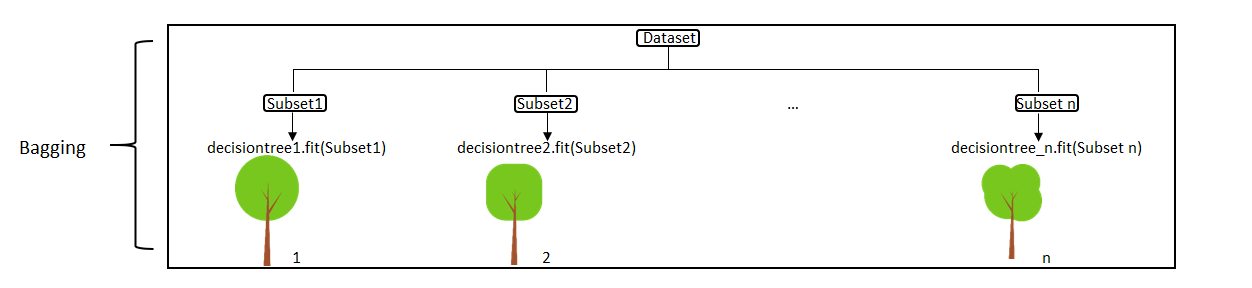
\includegraphics[width=16 cm]{images/bagging.png}
        \caption{Minh họa: Bagging}
        \label{fig:bagging}
    \end{figure}
    
    \subsubsection{Khái niệm: Random Forest}
    
    Random Forest \cite{breiman2001random}, hay còn gọi là Random Decision Forest, là một phương pháp ensemble, kết hợp nhiều mô hình cây quyết định phân lớp/hồi quy (Classification and regression trees - CART), cải tiến của phương pháp Bagging. RF được phát triển bởi Leo Breiman. Ông đồng thời cũng là tác giả của CART \cite{breiman_1984}
    
    \subsubsection{Mô tả thuật toán xây dựng Random Forest}
    
    \begin{itemize}
        \item Bước 1: Chọn ngẫu nhiên k từ n thuộc tính (k<n) có trong bộ dữ liệu huấn luyện.
        
        \item Bước 2: Sử dụng phương pháp boostrapping, chọn có hoàn lại từ bộ dữ liệu huấn luyện để tạo ra một bộ dữ liệu mới.
        
        \item Bước 3: Xây dựng cây quyết định với bộ dữ liệu ở bước 2, chỉ sử dụng k thuộc tính đã chọn ở bước 1
        
        \item Bước 4: Lặp lại Bước 2-3 để tạo nhiều cây quyết định khác.
        
        \item Bước 5: Kết hợp các cây quyết định thành phần bằng phương pháp bỏ phiếu.
    \end{itemize}
    
    \begin{figure}[htp]
        \centering
        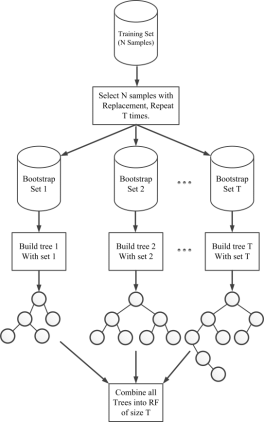
\includegraphics[width=8 cm, height=10cm]{images/Structure-of-random-forest.png}
        \caption{Minh họa: Random Forest \cite{RF_structure}}
        \label{fig:RF}
    \end{figure}
    
    \subsubsection{Dự đoán bằng Random Forest}
    
    Với x là một điểm dữ liệu mới, mỗi cây thành phần dự đoán hồi quy $T_{i}(x)$, dự đoán hồi quy của mô hình là:
    \begin{equation} \label{RF_reg}
        \hat{f}^{N}_{rf}(x) = \frac{1}{N} \underset{i=1}{ \overset{N}{\Sigma}} T_{i}(x)
    \end{equation}
    
    Với  $\hat{T}_{i}(x)$ là kết quả phân lớp của cây thành phần, dự đoán phân lớp của mô hình là:
    \begin{equation} \label{RF_cls}
        \hat{C}^{N}_{rf}(x) = majority \: vote \: \{\hat{T}_{i}(x)\}^{N}_{1}
    \end{equation}
    
    \subsubsection{Đánh giá Random Forest}
    
    Do sử dụng phương pháp boostrapping để tạo các mẫu huấn luyện cho các CART thành phần, chỉ có khoảng $\frac{2}{3}$ dữ liệu không trùng lặp trong bộ huấn luyện ban đầu được sử dụng cho việc huấn luyện. $\frac{1}{3}$ dữ liệu còn lại không tham gia huấn luyện được gọi là 'Out-of-bag dataset' (OOB). Phần dữ liệu này có thể xem như là một tập kiểm thử (validation dataset) dùng để đánh giá và tính toán độ quan trọng các thuộc tính của các CART trong rừng. Độ lỗi của RF trên tập dữ liệu OOB được gọi là 'Out-of-bag Error' ($E_{OOB}$).
    
    \begin{figure}[htp]
        \centering
        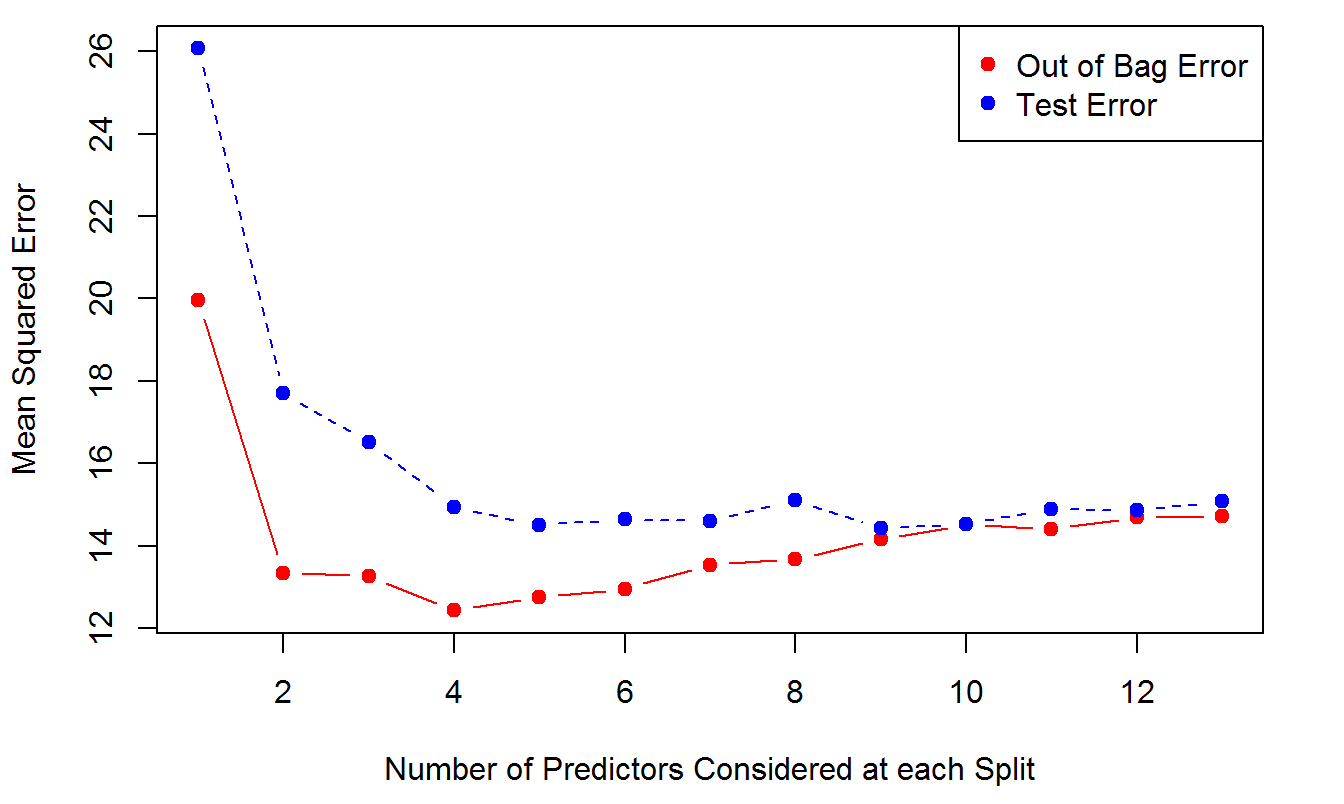
\includegraphics[width=12 cm]{images/rf_oob.png}
        \caption{Tương quan Out-of-bag error và test error}
        \label{fig:RF}
    \end{figure}
    
    Có thể so sánh $E_{OOB}$ giữa các RF có số thuộc tính được chọn k (ở bước 1) khác nhau và số lượng cây trong rừng khác nhau để chọn được mô hình RF có độ lỗi thấp nhất. 
    
    \subsubsection{Điểm mạnh của Random Forest}
    
    Thuật toán xây dựng có sự ngẫu nhiên trong mẫu dữ liệu (dùng phương pháp bootstrapping) và ngẫu nhiên trong số thuộc tính của mẫu so với tập thuộc tính ban đầu. Do đó, các tập huấn luyện con được tạo ra có tính đa dạng, ít liên quan. Mỗi CART xây dựng từ những tập dữ liệu con này không dùng tất cả dữ liệu training, cũng như không dùng tất cả các thuộc tính của dữ liệu để xây dựng nên mỗi cây có bias cao. Tuy nhiên, kết quả cuối của RF là kết hợp của nhiều cây thành phần, thông tin từ các cây sẽ bổ sung thông tin cho nhau, dẫn đến mô hình có low bias và low variance, tức là mô hình có kết quả dự đoán tốt.
    
    Trong rừng, mỗi cây thành phần chỉ được huấn luyện trên một tập nhỏ các thuộc tính thay vì toàn bộ (bước 1), cơ chế này giúp RF thực thi nhanh khi áp dụng trên tập dữ liệu có số lượng lớn thuộc tính. Hơn nữa, việc xây dựng từng cây thành phần là độc lập nên có thể dễ dàng thực hiện song song.


\subsection{Gradient Boosting (Tăng cường độ dốc)}
    \subsubsection{Khái niệm: Boosting}
        Boosting là một kỹ thuật ensemble với mục đích từ một số mô hình học yếu (weak learner) tạo ra mô hình học mạnh hơn (strong learner) bằng cách cho những mô hình sau sửa lỗi (học từ lỗi) của các mô hình trước. Các mô hình được thêm vào theo cách này cho đến khi đạt số lượng mô hình tối đa cho phép hoặc dự đoán hoàn toàn trùng khớp với tập huấn luyện.
        
        \begin{figure}[htp]
            \centering
            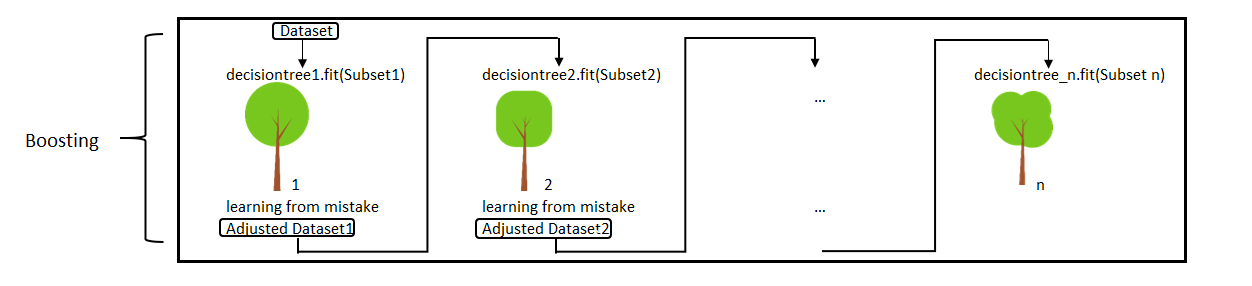
\includegraphics[width=16cm]{images/boosting.png}
            \caption{Minh họa: Boosting}
            \label{fig:boosting}
        \end{figure}
        
        Thuật toán boosting đơn giản nhất là Ada Boost, được giới thiệu vào năm 1995 bởi Freund và Schapire \cite{freund1997decision}.
        Thuật toán này sử dụng các CART có độ sâu nhỏ, hay còn gọi là một gốc (stump), làm các weak learner thành phần. 
        
        Ada Boost thực hiện việc học tăng cường bằng cách gán cho mỗi điểm dữ liệu trong bộ huấn luyện bộ huấn luyện một trọng số mẫu (sample wieght). Ban đầu, tất cả điểm dữ liệu đều được khởi tạo trọng số này bằng $\frac{1}{n}$, với n là tổng số điểm dữ liệu. Sau đó, với mỗi gốc được tạo, tổng lỗi của gốc đó sẽ quyết định trọng số của gốc trong việc bỏ phiếu (wieghted voting) cho kết quả dự đoán cuối. Những điểm dữ liệu cũng được cập nhật lại sample wieght dựa vào kết quả gốc hiện tại dự đoán đúng (sample wieght giảm) hay dự đoán sai (sample wieght tăng) thể hiện gốc sau đó cần dự thiết dự đoán đúng các điểm dữ liệu đang được dự đoán sai (gốc tiếp theo cố gắng sửa lỗi của gốc trước đó)
        
        Cụ thể thuật toán Ada Boost như sau \cite{freund1999short}:
        \begin{itemize}
            \item Khởi tạo $w_{1} = \{\frac{1}{N}\}^{N}_{1}$
            
            \item Với M là số gốc tối đa, lặp lại m=1,...M:
            \begin{itemize}
                \item Huấn luyện gốc sử dụng sample weight $w_{m}$
                
                \item Tính độ lỗi: 
                \begin{equation}
                    \epsilon_{t} = Pr_{i~D_{t}} [ h_{t} \ne y_{i} ]
                \end{equation}
                
                \item Thiết lập trọng số cho gốc này:
                    \begin{equation}
                        \alpha_{t} = \frac{1}{2}\ln{\frac{1 - \epsilon_{t}}{\epsilon_{t}}}
                    \end{equation}
                
                \item Cập nhật sample wieght cho việc huấn luyện gốc tiếp theo:
                    \begin{equation}
                        D_{t+1} = \frac{D_{t}(i)e^{-\alpha_{t}}}
                        {Z_{t}}
                    \end{equation}

                (với $Z_{t}$ là hệ số chuẩn hóa để tổng sample wieght bằng 1)
                
            \end{itemize}
            
            \item Cuối cùng, kết hợp các gốc bằng bỏ phiếu có trọng số:
                \begin{equation}
                    H(x) = sign( \underset{t=1}{ \overset{T}{\Sigma}} \alpha_{t} h_{t}(x) )
                \end{equation}
                \vspace{0.5cm}
    \clearpage
        \end{itemize}
        \clearpage
        \begin{figure}[H]
        \centering
        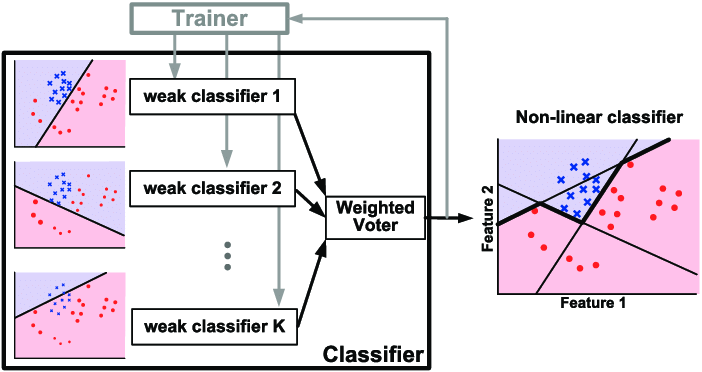
\includegraphics[width=8.5 cm,]{images/adaboost.png}
        \caption{Minh họa thuật toán AdaBoost, quá trình kết hợp các mô hình yếu \cite{adab_pic}}
        \label{fig:adab}
        \end{figure}
        
        
    \subsubsection{Gradient Boosting}
        Ý tưởng của thuật toán Gradient Boosting (GB) bắt nguồn từ Leo Breiman. Ông cho rằng phương pháp boosting có thể xem như là một thuật toán tối ưu hóa trên một hàm mất mát (Loss function) phù hợp \cite{breiman1997arcing}. Thuật toán Gradient boosting sau đó được phát triển bởi Jerome H. Friedman \cite{friedman2001greedy} \cite{friedman2002stochastic}.
        
        Khác với Ada Boost, ở Gradient Boosting:
            \begin{itemize}
                \item Sử dụng cây phân lớp, hồi quy làm các weaker learner thành phần thay vì gốc
            
                \item Những CART thành phần không huấn luyện dựa trên trọng số mẫu (mô hình tiếp theo cố gắng dự đoán đúng những điểm lỗi của mô hình trước), mà dựa trên  'độ lệch (lỗi) giả'(pseudo-residual) của CART tiền nhiệm trước đó (mô hình tiếp theo cố gắng giảm độ lỗi có được từ mô hình trước).
                
                \item Những mô hình thành phần không có trọng số riêng, thay vào đó chúng có chung một tỉ lệ tốc độ học (learning rate) trong khoảng {0-1} để điều chỉnh tốc độ học của từng mô hình mới.
            \end{itemize}
            
        Thuật toán kết thúc khi đạt số lượng cây tối đa hoặc việc thêm những cây mới không giảm pseudo-residual.
            
        \begin{figure}[htp]
        \centering
        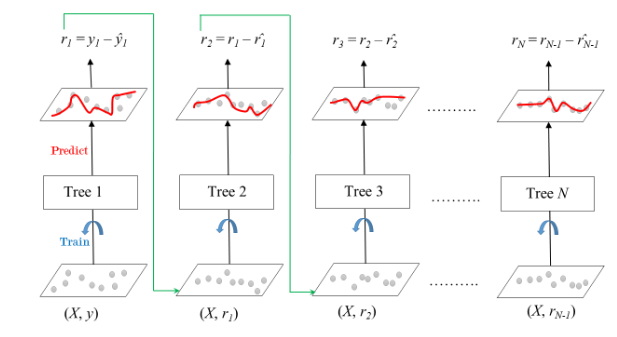
\includegraphics[width=10 cm,]{images/gradientboosting.png}
        \caption{Minh họa: Gradient boosting \cite{g4g_Gb}}
        \label{fig:gb}
        \end{figure}

        
    \subsubsection{Thuật toán Gradient Boosting \cite{starmer_2019_GBR} \cite{starmer_2019_GBC}:}
        
        Input: Dữ liệu huấn luyện $ \{(x_{i}, y_{i})\}^{n}_{i=1} $, một hàm Loss $ L(y, F(x)) $ và số lượng cây tối đa M
        \begin{itemize}
            \item Bước 1: Khởi tạo dự đoán ban đầu với hằng số
                \begin{equation}
                    F_{0}(x) = \underset{\gamma}{\mathrm{argmin}} \, 
                    \underset{i=1}{ \overset{n}{\Sigma}} L(y_{i}, \gamma)
                \end{equation}

            \item Bước 2: Lặp m=1 đến M để tạo M cây thành phần:
                \begin{description}
                    \item (A) Tính 'độ lệch giả' (pseudo-residual) của các điểm dữ liệu trong tập huấn luyện: Với mỗi i = 1, ..., n
                        \begin{equation}
                            r_{im} = -[\frac{\partial L(y_{i}, F(x_{i}))} {\partial F(x_{i})}]_{F(x) = F_{m-1}(x)}
                        \end{equation}
                        
                    \item (B) Xây dựng cây dự đoán các giá trị $r_{im}$, gọi $R_{jm}$ là các lá của cây, vớij=1, ...,$J_{m}$ (cây có $J_{m}$ lá)
                    
                    \item (C) Tính giá trị output ở từng lá của cây vừa tạo :
                        \begin{equation}
                            \gamma_{jm} = \underset{\gamma}{\mathrm{argmin}} \, 
                            \underset{x_{i} \in R_{ij}}{\Sigma}
                            L(y_{i}, F_{m-1}(x_{i}) + \gamma)
                        \end{equation}
                        
                    \item (D) Cập nhật dự đoán mới:
                        \begin{equation}
                            F_{m}(x) = F_{m-1}(x) + \nu \underset{j=1}{\overset{J_{m}}{\Sigma}}
                            \gamma_{m} I(x \in R{jm})
                        \end{equation}
                        với $\nu$ là tỷ lệ tốc độ học (learning rate)
                    
                \end{description}
                
        \end{itemize}
        
        Output: Kết quả dự đoán là kết quả của cây cuối cùng: $F_{M}(x)$
        
    \subsubsection{Điểm mạnh của Gradient Boosting}
        Qua mỗi cây mới được thêm vào, độ lỗi của mô hình sẽ ngày càng được giảm. Với các siêu tham số (hyperparameter) hợp lý, mô hình có thể cho được độ chính xác cao.
        
        \begin{figure}[htp]
        \centering
        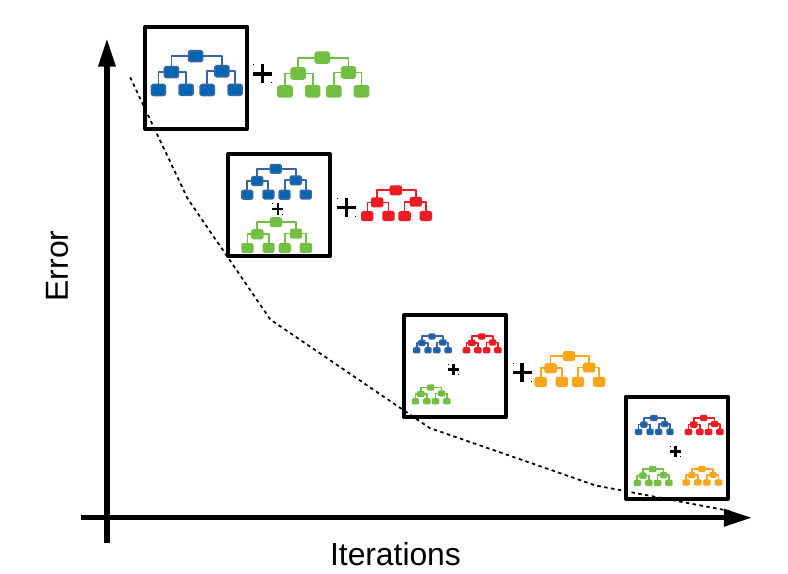
\includegraphics[width=10 cm,]{images/GB_error.png}
        \caption{Độ lỗi qua các iteration - GB \cite{gb_graph}}
        \label{fig:gb}
        \end{figure}
            
        Gradient Boosting có thể được tối ưu với nhiều hàm Loss khác nhau và cho phép hiệu chỉnh (fine tunning) nhiều siêu tham số (hyperparameter) giúp mô hình có độ linh hoạt cao giữa nhiều bộ dữ liệu khác nhau.


\subsection{XGBoost (Extreme Gradient Boosting)}
    XGBoost, viết tắt cho eXtreme Gradient Boosting, là một phiên bản Gradient Boosting được tối ưu hóa bởi Tianqi Chen \cite{chen2016xgboost}.
    
    Để cải tiến GB, mục tiêu của XGBoost không chỉ cố gắng tối thiểu hóa hàm Loss mà còn kèm theo một hàm chính quy hóa (regularization). Ta có thể gọi hàm mục tiêu (objective function) của XGBoost là: \cite{xgboost_model_tut}
    \begin{equation}
        obj(\theta) = \underset{i=1}{\overset{n}{\Sigma}} L(y_{i}, \hat{y}_{i}) + \underset{k=1}{\overset{K}{\Sigma}} \Omega(f_{k}) 
    \end{equation}
    với L là hàm Loss, $\Omega$ là hàm regularization, $f_{k}$ là mô hình thành phần thứ k. Việc thêm hàm regularization giúp cải tiến vấn đề overfit của mô hình Gradient Boosting, do sau mỗi lần thêm cây thành phần, độ lỗi của mô hình GB luôn được giảm cho đến tối thiểu hoặc mô hình đạt tối đa số cây thành phần.
    
    \subsubsection{Xây dựng CART trong mô hình XGBoost}
    Một trong những cải tiến của XGBoost so với Gradient Boost là ở việc tạo các cây hồi quy/phân lớp thành phần.
    
    Ở iteration thứ t, cây được tạo cho dự đoán 
    \begin{equation}
        \hat{y}_{i}^{(t)} =  \hat{y}_{i}^{(t-1)} + f_{t} (x_{i}) = \underset{k=1}{\overset{T}{\Sigma}}\Omega(f_{k}(x_{i}))
    \end{equation}
    
    Độ phức tạp của cây được định nghĩa là \cite{xgboost_model_tut}
    \begin{equation}
        \Omega(f) = \gamma T + \frac{1}{2} \lambda \underset{j=1}{\overset{T}{\Sigma}} w^{2}_{j}
    \end{equation}
    với $\gamma$ và $\lambda$ là các hệ số regularization, T là số lá của cây. Ta thấy $\underset{j=1}{\overset{T}{\Sigma}}w^{2}_{j}$ là tổng bình phương các lá, hay chính là tổng bình phương output của cây. Ta có thể đặt:
    
    \begin{equation}
        O^{2}_{value} = f_{t} (x_{i})^2 = \underset{j=1}{\overset{T}{\Sigma}}w^{2}_{j}
    \end{equation}
    
    khi đó độ phức tạp của cây là:
    \begin{equation}
        \Omega(f) = \gamma T + \frac{1}{2} \lambda  O^{2}_{value}
    \end{equation}
    
    Lúc này, hàm mục tiêu của XGBoost là \cite{xgboost_model_tut} \cite{starmer_2020_XGB}
    \begin{equation}
    \begin{split}
         obj^{(t)} & =  \underset{i=1}{\overset{n}{\Sigma}} L(y_{i}, \hat{y}_{i}^{(t-1)} + f_{t} (x_{i})) 
            + \Omega(f_{t}) + constant \\
           & = \underset{i=1}{\overset{n}{\Sigma}} L(y_{i}, \hat{y}_{i}^{(t-1)} + O_{value}) 
            + \gamma T + \frac{1}{2} \lambda  O^{2}_{value} + constant
    \end{split}
    \end{equation}
    
    Vậy, XGBoost chỉ thêm cây có output làm tối thiểu hóa được hàm mục tiêu này. Các hằng số sẽ không ảnh hưởng đến bài toán tối thiểu hóa nên ta có thể bỏ chúng đi
    \begin{equation}
         obj^{(t)} = \underset{i=1}{\overset{n}{\Sigma}} L(y_{i}, \hat{y}_{i}^{(t-1)} + O_{value}) 
         + \frac{1}{2} \lambda  O^{2}_{value}
    \end{equation}
    
    Áp dụng xấp xỉ Taylor bậc 2 (second order Taylor Approximation) \cite{Taylor_theorem}:
    
    \begin{equation}
    \begin{split}
        L(y_{i}, \hat{y}_{i}^{(t-1)} + O_{value}) \approx 
        L(y_{i}, \hat{y}_{i}^{(t-1)})
        & + \left[ \frac{d}{ d_{\hat{y}_{i}^{(t-1)}}}  L(y_{i}, \hat{y}_{i}^{(t-1)}) \right] O_{value} \\
        & + \frac{1}{2} \left[ \frac{d^{2}}{d^{2}_{\hat{y}_{i}^{(t-1)}}}  L(y_{i}, \hat{y}_{i}^{(t-1)}) \right] O^2_{value}
    \end{split}
    \end{equation}
    
    Đặt
    \begin{equation}
    \begin{split}
        & g = \left[ \frac{d}{ d_{\hat{y}_{i}^{(t-1)}}}  L(y_{i}, \hat{y}_{i}^{(t-1)}) \right]
        \\
        & h = \left[ \frac{d^{2}}{d^{2}_{\hat{y}_{i}^{(t-1)}}}  L(y_{i}, \hat{y}_{i}^{(t-1)}) \right]
    \end{split}
    \end{equation}
    
    Khi đó, hàm mục tiêu có thể được viết thành 
    \begin{equation}
        obj^{(t)} = \underset{i=1}{\overset{n}{\Sigma}} L(y_{i}, \hat{y}_{i}^{(t-1)})
        + \underset{i=1}{\overset{n}{\Sigma}} g_{i} O_{value}
        + \frac{1}{2} \underset{i=1}{\overset{n}{\Sigma}} h_{i} O^2_{value}
        + \frac{1}{2} \lambda O^2_{value}
    \end{equation}
    
    Ta thấy được $\underset{i=1}{\overset{n}{\Sigma}} L(y_{i}, \hat{y}_{i}^{(t-1)}) $ không chứa $O_{value}$, nên nó sẽ không ảnh hưởng đến quá trình tối thiểu hóa và có thể được bỏ đi. Hàm mục tiêu bây giờ là
    
    \begin{equation} \label{obj_func}
         obj^{(t)} = O_{value} \underset{i=1}{\overset{n}{\Sigma}} g_{i}
         + \frac{1}{2} O^2_{value} (\underset{i=1}{\overset{n}{\Sigma}} h_{i} + \lambda)
    \end{equation}
    
    Để tìm $O_{value}$ làm tối thiểu hàm mục tiêu, ta lấy đạo hàm hàm mục tiêu theo $O_{value}$ và tìm nghiệm bằng 0:
    
    \begin{equation} \label{eq_Ovalue}
        \begin{split}
            & \underset{i=1}{\overset{n}{\Sigma}} g_{i}
            + O_{value} (\underset{i=1}{\overset{n}{\Sigma}}h_{i} + \lambda) = 0 \\ \\
           	\Leftrightarrow \; &  O_{value} = - \frac{\underset{i=1}{\overset{n}{\Sigma}} g_{i}} {\underset{i=1}{\overset{n}{\Sigma}}h_{i} + \lambda}
        \end{split}
    \end{equation}
    
    \textbf{Ở bài toán hồi quy}, giả sử ta sử dụng hàm Loss MSE 
    $ L(y_{i}, \hat{y}_{i}^{(t-1)}) = \frac{1}{2} (y_{i} - \hat{y}_{i}^{(t-1)})^2 $, ta có thể tính $g_{i}$ và $h_{i}$
    \begin{equation}
        \begin{split}
        & g = -(y_{i} - \hat{y}_{i}^{(t-1)})
        \\
        & h = 1
        \end{split}
    \end{equation}
    
    thì hàm mục tiêu là:
    \begin{equation}
        O_{value} = \frac{\underset{i=1}{\overset{n}{\Sigma}} (y_{i} - \hat{y}_{i}^{(t-1)})}
        {\underset{i=1}{\overset{n}{\Sigma}}1 + \lambda}
    \end{equation}
    
    Ta thấy được ở phân số trên, tử số chính là tổng độ lỗi (sum of residuals) và mẫu số chính là tổng số phần tử trong kết quả (number of residuals) trong output + $\lambda$
    
    Vậy hàm mục tiêu của mô hình hồi quy này có thể hiểu là \cite{starmer_2020_XGB}
    \begin{equation}
        O_{value} = \frac{\text{Sum of Residuals}}
        {\text{Number of Residuals} + \lambda}
    \end{equation}
    
    Đây chính là công thức kết quả của một lá trên cây hồi quy.
    
    \textbf{Ở bài toán phân lớp}, giả sử ta sử dụng hàm Loss
    \begin{equation}
        L(y_{i}, \hat{y}_{i}^{(t-1)}) = -[ y_{i} \log(\hat{y}_{i}^{(t-1)}) + (1-y_{i})\log(1-\hat{y}_{i}^{(t-1)})]
    \end{equation}
    
    ta có thể tính $g_{i}$ và $h_{i}$ \cite{starmer_2020_XGB}
    \begin{equation}
        \begin{split}
        & g = -(y_{i} - \hat{y}_{i}^{(t-1)})
        \\
        & h = \hat{y}_{i}^{(t-1)}(1 - \hat{y}_{i}^{(t-1)})
        \end{split}
    \end{equation}
    
    thì hàm mục tiêu là:
    \begin{equation}
        O_{value} = \frac{\underset{i=1}{\overset{n}{\Sigma}} (y_{i} - \hat{y}_{i}^{(t-1)})}
        {\underset{i=1}{\overset{n}{\Sigma}}(\hat{y}_{i}^{(t-1)}(1 - \hat{y}_{i}^{(t-1)})) + \lambda}
    \end{equation}
    
    hay dễ hiểu chính là: \cite{starmer_2020_XGB}
    \begin{equation}
        O_{value} = \frac{\text{Sum of Residuals}}
        {\Sigma\text{[Previous Probability x (1 - Previous Probability)]} + \lambda}
    \end{equation}
    
    Đây chính là công thức kết quả của một lá trên cây phân lớp.
    
    \bigbreak
    
    \textbf{Tách lá ở cây}
    
    Ở XGBoost, khi tách một lá, ta dùng hàm Gain để xác định xem các cây con mới này phân cụm tốt hơn lá ban đầu hay không.
    \begin{equation} \label{eq_XBG_gain}
        \begin{split}
        \text{Gain} = \: & \text{Similarity Score}(\text{Lá trái}) 
        + \text{Similarity Score}(\text{Lá phải}) \\
        & - \text{Similarity Score}(\text{Gốc}) - \gamma
        \end{split}
    \end{equation}
    và tất nhiên cây con có Gain lớn nhất sẽ được chọn để tách lá.
    
    Công thức của Similarity Score (được miêu tả trong bản thảo XGBoost ban đầu \cite{chen2016xgboost}) ở hàm Gain trong XGBoost chính là âm của hàm mục tiêu đã được tối thiểu hóa.Tức là, để tính công thức Similarity Score, ta thế đáp án $O_{value}$ ta tính được ở \eqref{eq_Ovalue} vào \eqref{obj_func}
    \begin{equation}
        \begin{split}
        \text{Similarity Score} & = - \underset{i=1}{\overset{n}{\Sigma}} g_{i} (- \frac{\underset{i=1}{\overset{n}{\Sigma}} g_{i}} {\underset{i=1}{\overset{n}{\Sigma}}h_{i} + \lambda})
         - \frac{1}{2} (\underset{i=1}{\overset{n}{\Sigma}} h_{i} + \lambda) (- \frac{\underset{i=1}{\overset{n}{\Sigma}} g_{i}} {\underset{i=1}{\overset{n}{\Sigma}}h_{i} + \lambda})^2
        \\
        & = \frac{1}{2} \frac{(\underset{i=1}{\overset{n}{\Sigma}} g_{i})^2} {\underset{i=1}{\overset{n}{\Sigma}} h_{i} + \lambda}
        \end{split}
    \end{equation}
    Tuy nhiên, do Similarity Score là tương đối giữa các cây con và để giảm số tính toán cần thiết (tối ưu hóa), Similarity Score được áp dụng thực tế được bỏ đi phần $\frac{1}{2}$
    \begin{equation} \label{eq_XGB_sim}
        \text{Similarity Score} =  \frac{(\underset{i=1}{\overset{n}{\Sigma}} g_{i})^2} {\underset{i=1}{\overset{n}{\Sigma}} h_{i} + \lambda}
    \end{equation}
    
    Tương tự như cách tính $O_{value}$ cho bài toán hồi quy và phân lớp đã nêu ở trên, ta có thể tính được hàm Similarity Score với các hàm Loss khác nhau. Giả sử bài toán hồi quy và phần lớp sử dụng hàm Loss nêu trên, ta có thể tính hàm Similarity Score:
    
    \begin{equation}
        \text{Similarity Score} = \frac{(\underset{i=1}{\overset{n}{\Sigma}} (y_{i} - \hat{y}_{i}^{(t-1)}))^2}
        {\underset{i=1}{\overset{n}{\Sigma}}1 + \lambda}
    \end{equation}
    
    hay dễ hiểu chính là: \cite{starmer_2020_XGB}
    \begin{equation}
        \text{Similarity Score} = \frac{\text{(Sum of Residuals)}^2}
        {\text{Number of Residuals} + \lambda}
    \end{equation}
    
    cho hồi quy, và
    
    \begin{equation}
        \text{Similarity Score} = \frac{(\underset{i=1}{\overset{n}{\Sigma}} (y_{i} - \hat{y}_{i}^{(t-1)}))^2}
        {\underset{i=1}{\overset{n}{\Sigma}}(\hat{y}_{i}^{(t-1)}(1 - \hat{y}_{i}^{(t-1)})) + \lambda}
    \end{equation}
    
    hay dễ hiểu chính là: \cite{starmer_2020_XGB}
    \begin{equation}
        \text{Similarity Score} = \frac{\text{(Sum of Residuals)}^2}
        {\Sigma\text{[Previous Probability x (1 - Previous Probability)]} + \lambda}
    \end{equation}
    
    cho phân lớp.
    
    \bigbreak
    
    \textbf{Tỉa cành cây}
    
    Quay lại với hàm Gain \eqref{eq_XBG_gain} sau khi ta đã tính được công thức của Similariry Score \eqref{eq_XGB_sim}
    
    \begin{equation} \label{eq_XGB_Gain_final}
        \text{Gain} = \: \frac{(\underset{i=1}{\overset{n}{\Sigma}} g^{\text{Lá trái}}_{i})^2} {\underset{i=1}{\overset{n}{\Sigma}} h^{\text{Lá trái}}_{i} + \lambda} 
        + \frac{(\underset{i=1}{\overset{n}{\Sigma}} g^{\text{Lá phải}}_{i})^2} {\underset{i=1}{\overset{n}{\Sigma}} h^{\text{Lá phải}}_{i} + \lambda} 
        - \frac{(\underset{i=1}{\overset{n}{\Sigma}} g^{\text{Ngọn}}_{i})^2} {\underset{i=1}{\overset{n}{\Sigma}} h^{\text{Ngọn}}_{i} + \lambda} - \gamma
    \end{equation}
    
    Khi đã xây dựng xong cây, từ dưới lên trên, những nút đã tách lá nhưng cho Gain nhỏ hơn 0 sẽ bị 'tỉa cảnh' (tree pruning), gộp lại hai lá mà nút đó đã tách thành trở về một nút ban đầu. Tỉa cành ở đây giúp giảm độ phức tạp của các cây thành phần (regularization), giúp XGBoost giảm overfit
    
    Dựa vào công thức hàm Gain \eqref{eq_XGB_Gain_final}, ta thấy được hệ số regularization $\lambda$ và $\alpha$ càng cao thì việc tỉa cành sẽ càng mạnh.
    
\subsection {Logistic Classification (Hồi quy Logistic)}
\label{label:log_class}

Hồi quy Logistic (Logistic Regression) là một mô hình học máy tuyến tính dùng để giải quyết các bài toán \textbf{phân loại nhị phân}, trong đó đầu ra là một biến phân loại có hai trạng thái (ví dụ: 0/1, âm tính/dương tính).

\textbf{Ý tưởng chính}

Thay vì dự đoán một giá trị liên tục như hồi quy tuyến tính, Logistic Regression dự đoán xác suất một điểm dữ liệu thuộc về lớp dương (lớp 1), bằng cách sử dụng hàm sigmoid để biến đổi đầu ra thành giá trị trong khoảng \([0, 1]\).

\textbf{Công thức mô hình}

Cho đầu vào \( \mathbf{x} = (x_1, x_2, \ldots, x_n)^T \), và vector trọng số \( \mathbf{w} = (w_0, w_1, \ldots, w_n)^T \):

\begin{itemize}
    \item \textbf{Hàm dự đoán (sigmoid)}:
    \[
    \hat{y} = \sigma(z) = \frac{1}{1 + e^{-z}}, \quad \text{với } z = \mathbf{w}^T \mathbf{x} + b
    \]
    \item \textbf{Quy tắc phân loại}:
    \[
    \hat{y} \geq 0.5 \Rightarrow \text{lớp 1}; \quad \hat{y} < 0.5 \Rightarrow \text{lớp 0}
    \]
\end{itemize}

\textbf{Hàm mất mát (Binary Cross-Entropy)}

Hàm mất mát dùng để huấn luyện mô hình là:

\[
\mathcal{L}(\mathbf{w}) = -\frac{1}{m} \sum_{i=1}^{m} \left[ y^{(i)} \log \hat{y}^{(i)} + (1 - y^{(i)}) \log (1 - \hat{y}^{(i)}) \right]
\]

Trong đó:
\begin{itemize}
    \item \( m \): số mẫu trong tập huấn luyện
    \item \( y^{(i)} \): nhãn thực tế của mẫu thứ \( i \)
    \item \( \hat{y}^{(i)} \): xác suất dự đoán của mẫu thứ \( i \)
\end{itemize}

\textbf{Huấn luyện mô hình}

Trọng số \( \mathbf{w} \) được cập nhật qua thuật toán tối ưu như:
\begin{itemize}
    \item Gradient Descent
    \item Stochastic Gradient Descent
    \item Hoặc các trình tối ưu hóa hiện đại (Adam, RMSprop,...)
\end{itemize}

\textbf{Ưu điểm}

\begin{itemize}
    \item Mô hình đơn giản, dễ hiểu và dễ triển khai.
    \item Dự đoán xác suất thay vì chỉ nhãn.
    \item Hoạt động tốt với dữ liệu tuyến tính.
\end{itemize}

\textbf{Nhược điểm}

\begin{itemize}
    \item Không xử lý tốt các quan hệ phi tuyến (non-linear).
    \item Nhạy cảm với dữ liệu mất cân bằng giữa các lớp.
\end{itemize}

\textbf{Ứng dụng}

\begin{itemize}
    \item Phân loại email spam / không spam.
    \item Dự đoán khả năng khách hàng rời đi (churn prediction).
    \item Chẩn đoán y tế (ví dụ: bệnh có/không).
    \item Phân tích rủi ro tài chính (nợ xấu, vỡ nợ).
\end{itemize}

\subsection {K-Nearest Neighbors - KNN (Láng giềng gần nhất)}
\label{label:knn}

K-Nearest Neighbors (KNN) là một thuật toán học máy không tham số (non-parametric), sử dụng khoảng cách để phân loại hoặc dự đoán một điểm dữ liệu mới dựa trên các điểm gần nhất trong tập huấn luyện.

\textbf{Nguyên lý hoạt động}

\begin{enumerate}
    \item Tính khoảng cách từ điểm cần phân loại đến tất cả các điểm trong tập huấn luyện.
    \item Chọn ra \(k\) điểm gần nhất (nearest neighbors).
    \item Dự đoán nhãn của điểm mới dựa trên đa số nhãn (phân loại) hoặc trung bình (hồi quy) của \(k\) điểm gần nhất.
\end{enumerate}

\textbf{Công thức tính khoảng cách}

Phổ biến nhất là khoảng cách Euclid:

\[
d(\mathbf{x}, \mathbf{x}^{(i)}) = \sqrt{ \sum_{j=1}^n \left( x_j - x_j^{(i)} \right)^2 }
\]

Các lựa chọn khác:
\begin{itemize}
    \item Khoảng cách Manhattan:
    \[
    d(\mathbf{x}, \mathbf{x}^{(i)}) = \sum_{j=1}^n \left| x_j - x_j^{(i)} \right|
    \]
    \item Khoảng cách Minkowski (tổng quát):
    \[
    d(\mathbf{x}, \mathbf{x}^{(i)}) = \left( \sum_{j=1}^n \left| x_j - x_j^{(i)} \right|^p \right)^{1/p}
    \]
\end{itemize}

\textbf{Quy tắc phân loại}

\[
\hat{y} = \text{mode} \left( y^{(i_1)}, y^{(i_2)}, \dots, y^{(i_k)} \right)
\]

Trong đó:
\begin{itemize}
    \item \( \hat{y} \): nhãn dự đoán
    \item \( y^{(i)} \): nhãn của điểm lân cận thứ \(i\)
\end{itemize}

\textbf{Ưu điểm}

\begin{itemize}
    \item Dễ cài đặt và trực quan.
    \item Không cần huấn luyện mô hình (lazy learning).
    \item Phù hợp với bài toán phi tuyến.
\end{itemize}

\subsection*{Nhược điểm}

\begin{itemize}
    \item Tính toán chậm với dữ liệu lớn (phải tính khoảng cách với tất cả điểm huấn luyện).
    \item Nhạy cảm với nhiễu và thang đo dữ liệu (cần chuẩn hóa).
    \item Chọn \(k\) không phù hợp có thể gây quá khớp hoặc dưới khớp.
\end{itemize}

\textbf{Ứng dụng}

\begin{itemize}
    \item Nhận diện chữ viết tay (như MNIST).
    \item Dự đoán người dùng giống nhau trong hệ thống gợi ý.
    \item Phân loại bệnh, dữ liệu gen, khách hàng,...
\end{itemize}

\subsection {K-Means (Thuật toán phân cụm K trung bình)}
\label{label:kmean}
K-Means là một thuật toán học không giám sát phổ biến \cite{bishop2006pattern}, được sử dụng rộng rãi trong các bài toán phân cụm dữ liệu. Mục tiêu của K-Means là chia tập dữ liệu thành \textbf{K cụm} sao cho các điểm dữ liệu trong cùng một cụm có độ tương đồng cao với nhau và khác biệt rõ ràng với các cụm còn lại.

\subsubsection*{Nguyên lý hoạt động}

Thuật toán hoạt động theo các bước chính sau:

\begin{enumerate}
    \item \textbf{Khởi tạo:} Chọn ngẫu nhiên $K$ tâm cụm ban đầu (centroids).
    \item \textbf{Phân cụm:} Gán mỗi điểm dữ liệu vào cụm có tâm gần nhất (theo khoảng cách Euclidean).
    \item \textbf{Cập nhật:} Tính lại vị trí tâm cụm mới bằng trung bình các điểm trong cụm.
    \item \textbf{Lặp lại:} Quay lại bước 2 và 3 cho đến khi các tâm cụm hội tụ (không thay đổi đáng kể) hoặc đạt số vòng lặp tối đa.
\end{enumerate}

\subsubsection*{Công thức khoảng cách Euclidean}

Khoảng cách giữa điểm dữ liệu $x$ và tâm cụm $c$ được tính bằng công thức:

\[
d(x, c) = \sqrt{\sum_{i=1}^{n} (x_i - c_i)^2}
\]

Trong đó:
\begin{itemize}
    \item $x$: điểm dữ liệu.
    \item $c$: tâm cụm.
    \item $n$: số chiều của không gian dữ liệu.
\end{itemize}

\subsubsection*{Tham số quan trọng}

\begin{itemize}
    \item \textbf{K:} Số lượng cụm cần phân chia (phải được xác định trước).
    \item \textbf{Max iterations:} Số vòng lặp tối đa để thuật toán hội tụ.
    \item \textbf{Tolerance:} Ngưỡng thay đổi của tâm cụm để quyết định dừng thuật toán.
\end{itemize}

\subsubsection*{Ưu điểm}

\begin{itemize}
    \item Dễ hiểu và dễ triển khai.
    \item Tính toán nhanh, đặc biệt với dữ liệu lớn.
\end{itemize}

\subsubsection*{Hạn chế}

\begin{itemize}
    \item Nhạy cảm với vị trí khởi tạo tâm cụm.
    \item Phải biết trước số cụm $K$.
    \item Không hoạt động tốt với dữ liệu có hình dạng phức tạp hoặc phân bố chồng lấn.
\end{itemize}

\subsubsection*{Ứng dụng}

\begin{itemize}
    \item Phân đoạn khách hàng (customer segmentation).
    \item Nhóm ảnh trong xử lý ảnh (image clustering).
    \item Nhận dạng mẫu (pattern recognition).
    \item Nén ảnh (image compression).
\end{itemize}

\subsection {Spectral Clustering (Phân cụm phổ)}
\label{label:SpectralClustering}

Spectral Clustering (phân cụm phổ) \cite{868688} là một thuật toán phân cụm tiên tiến dựa trên lý thuyết đồ thị và đại số tuyến tính. Thay vì phân cụm trực tiếp trên không gian dữ liệu, thuật toán này chuyển dữ liệu sang một không gian mới thông qua việc phân tích các giá trị riêng (eigenvalues) và vector riêng (eigenvectors) của một ma trận biểu diễn quan hệ giữa các điểm dữ liệu.

\subsubsection*{Nguyên lý hoạt động}

Spectral Clustering hoạt động thông qua các bước chính sau:

\begin{enumerate}
    \item \textbf{Xây dựng ma trận kề (Adjacency Matrix)}: Xác định mức độ liên kết giữa các điểm dữ liệu (thường dùng khoảng cách Gaussian hoặc k-NN).
    \item \textbf{Tính ma trận Laplacian}: Từ ma trận kề, tính ma trận Laplacian $L = D - A$, trong đó $D$ là ma trận bậc (degree matrix) và $A$ là ma trận kề.
    \item \textbf{Phân tích giá trị riêng}: Tính các vector riêng tương ứng với $k$ giá trị riêng nhỏ nhất (hoặc lớn nhất tuỳ loại Laplacian).
    \item \textbf{Ánh xạ không gian mới}: Biểu diễn mỗi điểm dữ liệu theo các vector riêng.
    \item \textbf{Áp dụng phân cụm K-Means}: Áp dụng thuật toán K-Means trong không gian mới này để phân chia cụm.
\end{enumerate}

\subsubsection*{Ưu điểm}
\begin{itemize}
    \item Phân cụm tốt cho dữ liệu có hình dạng phức tạp, không lồi.
    \item Không yêu cầu giả định phân phối dữ liệu.
    \item Có thể áp dụng cho dữ liệu biểu diễn dưới dạng đồ thị.
\end{itemize}

\subsubsection*{Hạn chế}
\begin{itemize}
    \item Hiệu suất kém với dữ liệu lớn (do tính toán ma trận và phân tích trị riêng).
    \item Cần chọn tham số phù hợp: số cụm $k$, hàm tương đồng, và tham số Gaussian $\sigma$.
\end{itemize}

\subsubsection*{Ứng dụng}
\begin{itemize}
    \item Phân tích mạng xã hội.
    \item Phân đoạn ảnh trong thị giác máy tính.
    \item Nhận dạng cộng đồng (community detection) trong đồ thị.
\end{itemize}

\subsection {Gaussian Mixture Model - GMM (Mô hình hỗn hợp Gauss)}
\label{label:SpectralClustering}

Gaussian Mixture Model (GMM) \cite{bishop2006pattern} là một mô hình xác suất dùng để biểu diễn sự phân bố của dữ liệu như là sự kết hợp của nhiều phân phối Gaussian (chuẩn) khác nhau. GMM là một phương pháp phân cụm dựa trên mô hình (model-based clustering), cho phép mô hình hóa các cụm có hình dạng ellipsoid và phân bố chồng lấn.

\subsubsection*{Nguyên lý hoạt động}

GMM giả định rằng dữ liệu được tạo ra từ sự kết hợp của $K$ phân phối Gaussian. Mỗi điểm dữ liệu có xác suất thuộc về mỗi Gaussian khác nhau, thay vì gán cứng vào một cụm như K-Means.

Xác suất tổng hợp của một điểm dữ liệu $x$ là:

\[
p(x) = \sum_{k=1}^{K} \pi_k \cdot \mathcal{N}(x \mid \mu_k, \Sigma_k)
\]

Trong đó:
\begin{itemize}
    \item $\pi_k$: trọng số (mixing coefficient) của thành phần thứ $k$ ($\sum \pi_k = 1$).
    \item $\mu_k$: vector trung bình của phân phối Gaussian thứ $k$.
    \item $\Sigma_k$: ma trận hiệp phương sai của phân phối Gaussian thứ $k$.
    \item $\mathcal{N}(x \mid \mu_k, \Sigma_k)$: phân phối chuẩn đa biến.
\end{itemize}

\subsubsection*{Thuật toán ước lượng tham số: EM (Expectation-Maximization)}

\begin{enumerate}
    \item \textbf{E-step (Expectation):} Tính xác suất mỗi điểm thuộc về từng thành phần Gaussian (trách nhiệm).
    \item \textbf{M-step (Maximization):} Cập nhật các tham số $\pi_k$, $\mu_k$, và $\Sigma_k$ để cực đại hóa log-likelihood.
    \item \textbf{Lặp lại} cho đến khi hội tụ.
\end{enumerate}

\subsubsection*{Ưu điểm}

\begin{itemize}
    \item Mô hình được các cụm phức tạp hơn hình cầu (so với K-Means).
    \item Gán mềm (soft clustering), mỗi điểm có thể thuộc nhiều cụm với các xác suất khác nhau.
\end{itemize}

\subsubsection*{Hạn chế}

\begin{itemize}
    \item Nhạy cảm với khởi tạo ban đầu.
    \item Dễ bị rơi vào cực trị cục bộ.
    \item Hiệu suất giảm với dữ liệu có chiều cao.
\end{itemize}

\subsubsection*{Ứng dụng}

\begin{itemize}
    \item Nhận dạng giọng nói và âm thanh.
    \item Phân đoạn ảnh (image segmentation).
    \item Hệ thống khuyến nghị.
    \item Phát hiện dị thường (anomaly detection).
\end{itemize}

\subsection{LSTM (Long Short-Term Memory)}
    \subsubsection{Artificial Neural Network (ANN)}
    Artificial Neural Network hay mạng thần kinh nhân tạo, gọi tắt là mạng thần kinh hoặc mạng neural, là một mô hình xử lý thông tin lấy cảm hứng từ  mạng neural sinh học. Kiến trúc của một mạng neural gồm 3 thành phần đó là lớp vào - input layer, lớp ẩn - hidden layer và lớp ra - output layer. Lưu ý, một mạng neural có thể chứa nhiều lớp ẩn ở giữa lớp vào và lớp ra.
    \begin{figure}[htp]
        \centering
        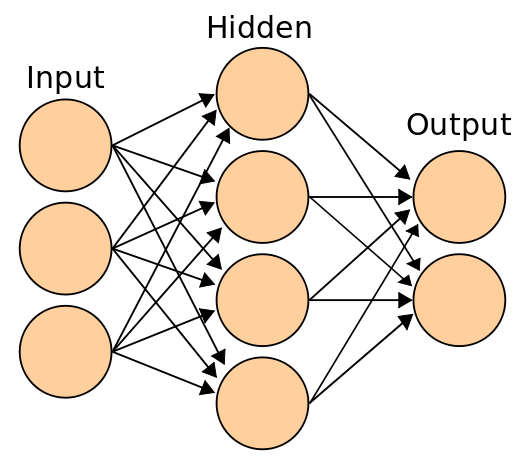
\includegraphics[width=6 cm]{images/ann.png}
        \caption{Minh họa cấu trúc của một mạng neural. \cite{ann_struct}}
        \label{fig:ann_structure}
    \end{figure}
    
    Ta có thể mô tả hoạt động mạng neural bằng công thức
    \begin{equation} \label{ann_eqn}
        y^{(l)}_i = f^{(l)}_i\left(\sum_{j=1}^{n^{(l-1)}}w^{(l)}_{ij}y^{(l-1)}_{j} + b^{(l)}_i\right).
    \end{equation}
    Trong đó:
    \begin{itemize}
        \item $l=1\dotsc L$, với $L$ là số lớp của mạng và $n^l$ là số neural ở lớp thứ $l$.
        \item $y^{(l)}_i$ là đầu ra của neural thứ $i$ ở lớp thứ $l$, với $i = 1\dotsc n^{l}$.
        \item $f^{(l)}_i$ là hàm truyền của neural thứ $i$ ở lớp thứ $l$. Hàm truyền tồn tại nhiều lựa chọn và mỗi lựa chọn có ảnh hưởng lớn đến kết quả đầu ra của mạng.
        \item $w_{i}^{(l)}$ là trọng số của đầu vào thứ $i$ ở lớp thứ $l$ thể hiện độ mạnh của từng đầu vào đối với quá trình xử lý thông tin để chuyển đổi dữ liệu từ lớp này sang lớp khác.
        \item Đầu vào của mạng là $y^{(0)} = \textbf{x}$ và đầu ra cuối là $\textbf{y} = y^{(L)}$.
        \item $b^{(l)}_i$ là \textit{ngưỡng} (bias) của neural thứ $i$ ở lớp thứ $l$.
    \end{itemize}
    
    Như vậy, quá trình học của mạng neural là quá trình tìm bộ trọng số $\textbf{w}$ sao cho phù hợp nhất. Quá trình này sẽ lặp liên tục và có thể không dừng đến khi tìm ra kết quả như ý. Vì vậy, trong thực tế, khi huấn luyện một mô hình mạng neural, một tiêu chuẩn dựa trên một giá trị sai số nào giữa đầu ra của mạng và đầu ra mong muốn cần được thiết lập, hoặc một số lần lặp tối đa xác định nào đó. Từ đây, ta tiếp cận thuật toán lan truyền ngược (Backpropagation), được sử dụng để điều chỉnh các trọng số liên kết sao cho tổng sai số nhỏ nhất. Với các mạng neural hiện đại, giải thuật được sử dụng kết hợp với một phương pháp tối ưu hóa như gradient descent để rút ngắn thời gian chạy của mạng.
    
    \subsubsection{Backpropagation}
    Trước hết, Gradient descent là một thuật toán tìm giá trị nhỏ nhất của hàm số f(x) dựa trên đạo hàm của nó. Thuật toán gồm 3 bước chính: (1) Khỏi tạo giá trị $x = x_0$ tùy ý; (2) Tính $x_1 = x_0 - \eta f'(x_0)$, với $\eta$ là \textit{learning rate} (tạm dịch là tốc độ học); (3) Tính lại $f(x)$ với các giá trị $x$ mới, sao cho nếu $f(x)$ đủ nhỏ thì dừng lại, còn không, lặp lại bước (2) với $x_2, x_3,\dotsc$
    
    Ta có thể nói, thuật toán lan truyền ngược áp dụng Stochastic Gradient Descent (gradient descent ngẫu nhiên - SGD) cho mạng neural có mục tiêu là tìm giá trị nhỏ nhất cho hàm $e(\textbf{w})$ qua đạo hàm $\nabla e(\textbf{w}): \dfrac{\partial e(\textbf{w})}{\partial w^{(l)}_{ij}}$ với toàn bộ $i, j, l$. Điểm khác biệt lớn của SGD là bước khởi tạo toàn bộ các trọng số sẽ khởi tạo ngẫu nhiên để tránh \textit{bias}.
    
    \subsubsection{Recurrent Neural Network (RNN)}
    Hình \ref{fig:ann_structure} ở phần trước là một ví dụ cho \textit{mạng neural nhân tạo truyền thẳng} (Feedforward Neural Network - FNN) gồm hai lớp ẩn kết nối hoàn toàn với nhau ở mỗi nút. Kiến trúc mạng truyền thẳng như trên không có các kết nối ngược trở lại từ các neural đầu ra về các neural đầu vào và mạng không lưu lại các giá trị output trước cũng như các trạng thái kích hoạt của neural. 
    
    Một kiểu kiến trúc khác là kiến trúc phản hồi (feedback), hay còn có tên là mạng neural hồi quy (Recurrent Neural Networ - RNN) cho phép đưa tín hiệu theo cả hai hướng thẳng và ngược lại bằng các vòng lặp. Mạng lưu lại các trạng thái trước đó, và hơn nữa, các trạng thái tiếp theo không chỉ phụ thuộc vào các tín hiệu đầu vào, mà còn phụ thuộc vào các trạng thái trước đó của mạng. Ý tưởng đằng sau RNN là RNN giống như trí nhớ ngắn hạn (Short Term Memory - STM) trong não người, tức là, RNN sẽ "học" và "ghi nhớ" lại thông tin ở chu kì trước và áp dụng ở bước "học" tiếp theo.
    \clearpage
    \begin{figure}[htp]
        \centering
        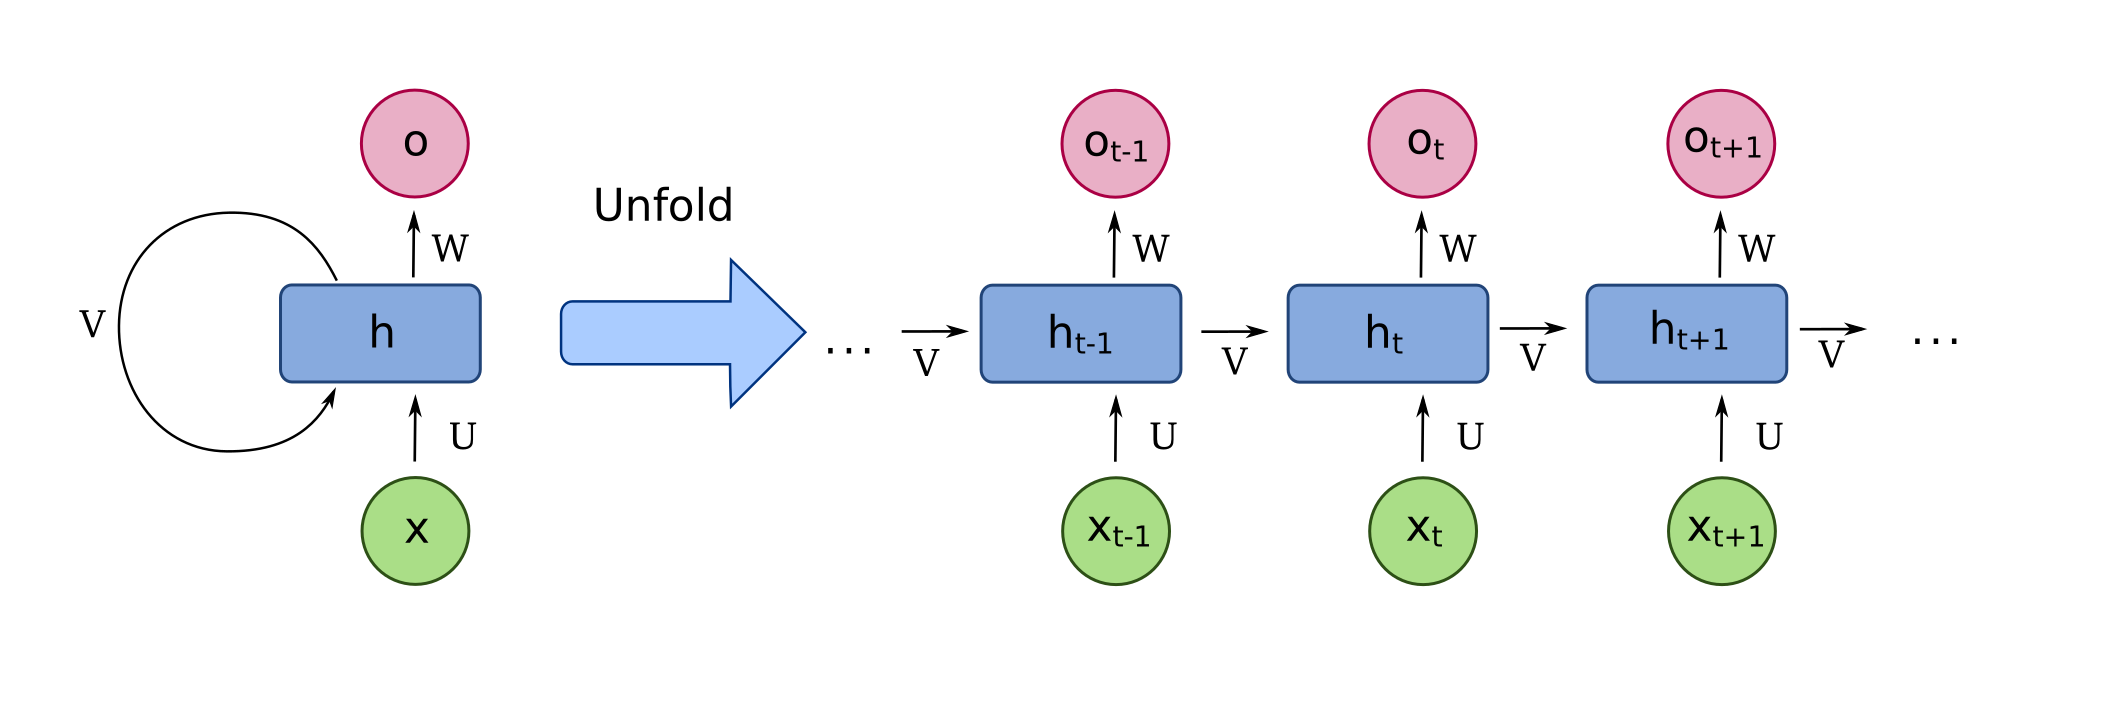
\includegraphics[width=15 cm]{images/rnn_unfold.png}
        \caption{Mô hình mạng neural hồi quy. \cite{rnn_unfold}}
        \label{fig:rnn_unfold}
    \end{figure}
    
    Dựa theo hình \ref{fig:rnn_unfold}, trong đó, $x_t$ và $o_t$ lần lượt là đầu vào và đầu ra tại thời điểm thứ $t$, $h_t$ là trạng thái ẩn tại thời điểm thứ $t$ và đóng vai trò là bộ nhớ của mạng. $h_t$ sẽ được tính dựa trên sự kết hợp giữa các trạng thái ẩn trước và đầu vào. Ta có thể viết:
    $$h_t = f(Ux_t + VS_{t-1}).$$
    
    Sau đó, $o_t$ sẽ được tính dựa theo $Wh_t$, với $(U, V, W)$ là ba tham số của mạng. Hai loại hàm truyền $f$ phổ biến nhất là hàm tanh hoặc hàm ReLU.
    
    Với khả năng “nhớ” được, mạng neural hồi quy được sử dụng để xử lý thông tin dạng chuỗi và các dữ liệu thời gian. Một số ứng dụng tiêu biểu là: mô hình ngôn ngữ và phát sinh văn bản, dịch máy (Machine Translation) và phát sinh mô tả cho ảnh (Generating Image Descriptions).
    
    \subsubsection{Hạn chế của RNN}
    Việc huấn luyện một RNN, cũng tương tự như mạng bình thường, sẽ sử dụng lan truyền ngược - Backpropagation như trên. Tuy nhiên, do bản chất có bộ nhớ của RNN, quá trình lan truyền ngược này sẽ được thực hiện qua từng thời điểm trong mạng. Quá trình này được gọi là \textit{lan truyền ngược liên hồi} (backpropagation through time).
    
    Mục tiêu là tính đạo hàm của lỗi với tham số $(U, V, W)$ tương ứng, sau đó, học các tham số này bằng cách sử dụng gradient descent. Ta có, ở từng trạng thái $h$, đạo hàm của hàm lỗi được khai triển như sau:
    $$\sum_t\dfrac{\partial e_t(\textbf{w})}{\partial\textbf{w}}\propto\sum_t\left(\prod_{i=k+1}\dfrac{\partial h_i}{\partial h_{i-1}}\right)\dfrac{\partial h_k}{\partial\textbf{w}}.$$
    
    Giả sử, trong trường hợp giá trị $\left\|\dfrac{\partial h_i}{\partial h_{i-1}}\right\|_2 < 1$, giá trị cập nhật sẽ bị giảm về gần 0 rất nhanh. Ví dụ, nếu lượng cập nhật chỉ là 0.01, nhưng qua 100 thời điểm, thì giá trị trên sẽ là $0.01^{100} \approx 0$. Mà khi đạo hàm bằng 0 thì có nghĩa là xảy ra hiện tượng bão hòa dẫn đến các nút phía trước cũng sẽ bị bão hoà theo. Vấn đề này không chỉ xảy ra với mạng RNN mà ngay cả mạng neural thường khá sâu cũng có hiện tượng này. Người ta gọi đây là hiện tượng \textbf{mất mát đạo hàm} (vanishing gradient).
    
    Một phương pháp phổ biến để giải quyết tình trạng mất mát đạo hàm là sử dụng kiến trúc mạng nhớ dài-ngắn hạn (Long Short-Term Memory (LSTM)). 
    
    \subsubsection{Long Short-Term Memory (LSTM)}
    \begin{figure}[htp]
        \centering
        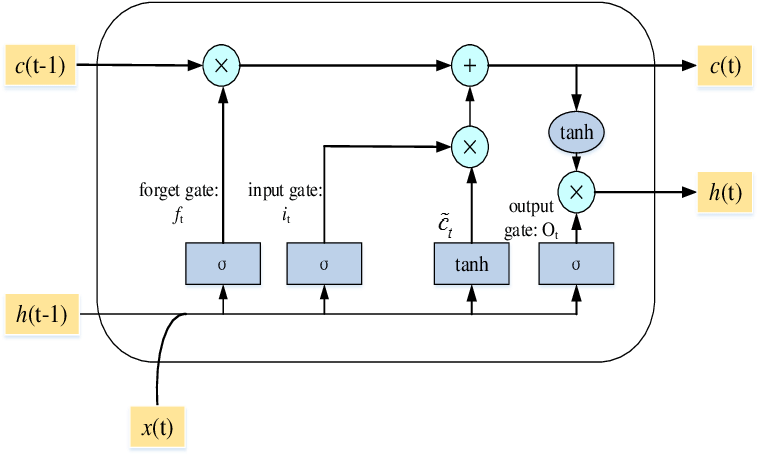
\includegraphics[width=14 cm]{images/lstm_struct.png}
        \caption{Cấu trúc của LSTM. \cite{lstm_struct}}
        \label{fig:lstm_struct}
    \end{figure}
    LSTM là một mô hình cải tiến của RNN và có cấu trúc tương tự nhưng khác ở cách tính toán đối với các trạng thái ẩn. Mấu chốt của khả năng “nhớ lâu” của LSTM là cấu trúc “trạng thái nhớ”. Ngoài ra, quá trình thêm hoặc loại bỏ thông tin sẽ dựa trên qui định của các cổng. Tóm lại, cốt lõi của mạng LSTM bao gồm trạng thái nhớ và các cổng.
    
    Các cổng của LSTM là một phương pháp định nghĩa thông tin băng qua và chúng được tạo bắng hàm sigmoid $\sigma$. Cụ thể, hàm sigmoid có giá trị thuộc khoảng (0, 1) mang ý nghĩa độ lớn thông tin được phép truyền qua tại mỗi lớp mạng. Nếu kết quả là 0,  điều này có nghĩa là không thông tin nào được phép đi qua, và ngươc lại, 1 nghĩa là toàn bộ thông tin được đi qua.
    
    Một mạng LSTM có 3 loại cổng, đều có đầu vào là trạng thái trước, đặt tên là $S \in \{h, c\}$, và đầu vào, nhân với trọng số tương ứng. Lưu ý, các cổng sẽ nhận một loại trọng sô khác nhau:
    \begin{itemize}
        \item \textbf{Cổng quên (Forget gate)} $f_t = \sigma(W_fS_{t-1} + W_fX_t)$.
        \item \textbf{Cổng vào (Input gate)} $i_t = \sigma(W_iS_{t-1} + W_iX_t)$
        \item \textbf{Cổng ra (Output gat)} $o_t = \sigma(W_oS_{t-1} + W_oX_t)$
    \end{itemize}
    
    Sau đó, trạng thái nhớ trung gian có thể được tính bằng hàm tanh qua công thức $\Tilde{C}_t = \text{tanh}(W_cS_{t-1} + W_cX_t)$. Từ đây, \textbf{trạng thái nhớ} sẽ nhận trạng thái trung gian và trạng thái nhớ trước, kết hợp với cổng vào và cổng quên như sau:
    \begin{equation} \label{lstm_cell_state_eqn}
        c_t = (i_t\times\Tilde{C}_t) + (f_t\times c_{t - 1}).
    \end{equation}
    
    Cuối cùng, trạng thái ẩn sẽ được tính bằng hàm tanh của trạng thái nhớ nhân với cổng ra:
    \begin{equation} \label{lstm_hidden_state_eqn}
        h_t = o_t\times\text{tanh}(c_t).
    \end{equation}
    
    Lưu ý, phép nhân trong công thức \ref{lstm_cell_state_eqn} và \ref{lstm_hidden_state_eqn} phụ thuộc vào $S$, tức là, các cổng sẽ thực hiện tính cho cả $h$ và $c$, sau đó, thực hiện phép nhân tương ứng cho mỗi loại trạng thái.

\section{Giới thiệu các bộ chuẩn hóa dữ liệu} \label{sec:basis-scaler}
\subsection {Chuẩn hóa dữ liệu với Min-Max Scaler}
\label{scaler:minmax}

Trong học máy, việc chuẩn hóa dữ liệu đầu vào giúp mô hình học hiệu quả hơn, đặc biệt với các mô hình nhạy cảm với thang đo (như KNN, SVM, hồi quy Logistic, mạng nơ-ron,...).

Một trong các phương pháp chuẩn hóa phổ biến là \textbf{Min-Max Scaling}, hay còn gọi là \textit{feature normalization}.

\textbf{Công thức Min-Max Scaling}

\[
x_i^{\text{scaled}} = \frac{x_i - x_{\min}}{x_{\max} - x_{\min}}
\]

Trong đó:
\begin{itemize}
    \item \( x_i \): giá trị gốc của đặc trưng.
    \item \( x_{\min} \): giá trị nhỏ nhất của đặc trưng trong tập dữ liệu.
    \item \( x_{\max} \): giá trị lớn nhất của đặc trưng.
    \item \( x_i^{\text{scaled}} \): giá trị sau khi chuẩn hóa.
\end{itemize}

\textbf{Ý nghĩa}

Min-Max Scaler biến đổi các đặc trưng về khoảng giá trị \([0, 1]\), giúp:

\begin{itemize}
    \item Tăng tốc độ hội tụ của thuật toán tối ưu.
    \item Tránh hiện tượng một vài đặc trưng chi phối quá trình học do thang đo lớn.
    \item Dữ liệu có cùng thang đo, phù hợp với các mô hình tính toán khoảng cách.
\end{itemize}

\textbf{Ví dụ}

Cho tập dữ liệu: \( x = [20, 40, 60, 80, 100] \)

\begin{itemize}
    \item \( x_{\min} = 20 \), \( x_{\max} = 100 \)
    \item \( x_3 = 60 \Rightarrow x_3^{\text{scaled}} = \frac{60 - 20}{100 - 20} = \frac{40}{80} = 0.5 \)
\end{itemize}

\textbf{Lưu ý}

\begin{itemize}
    \item Cần áp dụng giá trị \( x_{\min}, x_{\max} \) từ tập huấn luyện cho cả tập kiểm tra.
    \item Không nên dùng Min-Max Scaling nếu dữ liệu chứa nhiều ngoại lệ (nên dùng Robust Scaler).
\end{itemize}

\subsection{Chuẩn hóa dữ liệu với Standard Scaler}
\label{scaler:standard}

Trong học máy, việc chuẩn hóa dữ liệu giúp các mô hình hoạt động hiệu quả hơn, đặc biệt với các thuật toán nhạy cảm với độ lớn của đặc trưng như: hồi quy Logistic, KNN, SVM, mạng nơ-ron,...

Một kỹ thuật chuẩn hóa phổ biến là \textbf{Standard Scaler} – biến đổi dữ liệu sao cho có trung bình bằng 0 và độ lệch chuẩn bằng 1.

\textbf{Công thức chuẩn hóa Standard Scaler}

\[
x_i^{\text{scaled}} = \frac{x_i - \mu}{\sigma}
\]

Trong đó:
\begin{itemize}
    \item \( x_i \): giá trị gốc của đặc trưng.
    \item \( \mu \): trung bình (mean) của đặc trưng.
    \item \( \sigma \): độ lệch chuẩn (standard deviation).
    \item \( x_i^{\text{scaled}} \): giá trị sau khi chuẩn hóa.
\end{itemize}

\textbf{Ý nghĩa}

\begin{itemize}
    \item Dữ liệu sau chuẩn hóa có phân phối chuẩn hóa chuẩn: \( \mathcal{N}(0, 1) \).
    \item Trung bình bằng 0 và phương sai bằng 1 giúp mô hình học ổn định hơn.
\end{itemize}

\textbf{Ví dụ}

Cho tập dữ liệu: \( x = [10, 12, 14, 16, 18] \)

\begin{itemize}
    \item Trung bình \( \mu = 14 \), độ lệch chuẩn \( \sigma = \sqrt{\frac{(4^2 + 2^2 + 0^2 + 2^2 + 4^2)}{5}} = \sqrt{8} \approx 2.828 \)
    \item \( x_1^{\text{scaled}} = \frac{10 - 14}{\sigma} \approx \frac{-4}{2.828} \approx -1.414 \)
\end{itemize}

\textbf{Lưu ý}

\begin{itemize}
    \item Nên tính \( \mu \) và \( \sigma \) trên tập huấn luyện, rồi áp dụng lên cả tập kiểm tra.
    \item Phù hợp nếu dữ liệu có phân phối gần chuẩn.
    \item Không phù hợp khi có nhiều ngoại lệ → khi đó dùng RobustScaler.
\end{itemize}

\subsection{Chuẩn hóa dữ liệu với Robust Scaler}
\label{scaler:robust}

\textbf{Robust Scaler} là một kỹ thuật chuẩn hóa dữ liệu giúp giảm ảnh hưởng của các giá trị ngoại lệ (outliers). Khác với Min-Max Scaler (dựa trên max/min) hay Standard Scaler (dựa trên trung bình/độ lệch chuẩn), Robust Scaler sử dụng các số liệu thống kê mạnh như \textbf{trung vị} (median) và \textbf{IQR – khoảng tứ phân vị}.

\textbf{Công thức chuẩn hóa}

\[
x_i^{\text{scaled}} = \frac{x_i - \text{Median}(x)}{\text{IQR}(x)}
\]

Trong đó:
\begin{itemize}
    \item \( \text{Median}(x) \): trung vị của đặc trưng.
    \item \( \text{IQR}(x) = Q_3 - Q_1 \): khoảng tứ phân vị (Interquartile Range), với:
        \begin{itemize}
            \item \( Q_1 \): phân vị thứ 25\% (lower quartile)
            \item \( Q_3 \): phân vị thứ 75\% (upper quartile)
        \end{itemize}
    \item \( x_i^{\text{scaled}} \): giá trị sau chuẩn hóa.
\end{itemize}

\textbf{Ưu điểm}

\begin{itemize}
    \item Không bị ảnh hưởng mạnh bởi ngoại lệ.
    \item Giữ nguyên phân phối cơ bản của dữ liệu phần lớn.
    \item Phù hợp với các mô hình yêu cầu dữ liệu chuẩn hóa như KNN, SVM, Logistic Regression.
\end{itemize}

\textbf{Ví dụ}

Giả sử đặc trưng \( x = [10, 12, 14, 16, 100] \)

\begin{itemize}
    \item \( \text{Median}(x) = 14 \)
    \item \( Q_1 = 12, Q_3 = 16 \Rightarrow \text{IQR} = 4 \)
    \item \( x_5^{\text{scaled}} = \frac{100 - 14}{4} = 21.5 \)
    \item Trong khi Min-Max sẽ nén dữ liệu về [0,1], nhưng sẽ bị kéo lệch vì 100 là ngoại lệ.
\end{itemize}

\textbf{Lưu ý}

\begin{itemize}
    \item Nên tính Median và IQR từ tập huấn luyện và áp dụng cho tập kiểm tra.
    \item Không thích hợp nếu dữ liệu đã phân bố chuẩn và không có ngoại lệ → dùng StandardScaler.
\end{itemize}

\subsection{Chuẩn hóa dữ liệu với MaxAbsScaler}
\label{scaler:maxabs}

\textbf{MaxAbsScaler} là một kỹ thuật chuẩn hóa dữ liệu theo phương pháp co dãn tuyến tính (linear scaling), sử dụng giá trị tuyệt đối lớn nhất trong từng đặc trưng để đưa dữ liệu về khoảng \([-1, 1]\), mà vẫn giữ nguyên dấu gốc của dữ liệu.

\textbf{Công thức chuẩn hóa}

\[
x_i^{\text{scaled}} = \frac{x_i}{\max \left( |x| \right)}
\]

Trong đó:
\begin{itemize}
    \item \( x_i \): giá trị ban đầu của đặc trưng.
    \item \( \max(|x|) \): giá trị tuyệt đối lớn nhất trong đặc trưng đó.
    \item \( x_i^{\text{scaled}} \): giá trị sau chuẩn hóa, nằm trong khoảng \( [-1, 1] \).
\end{itemize}

\textbf{Đặc điểm}

\begin{itemize}
    \item Dữ liệu được chia cho giá trị tuyệt đối lớn nhất, nên không làm thay đổi sparsity (độ thưa).
    \item Giữ nguyên dấu ban đầu của dữ liệu.
    \item Thích hợp với dữ liệu có giá trị cả âm và dương, đặc biệt là dữ liệu sparse (rất nhiều giá trị 0).
\end{itemize}

\textbf{Ví dụ}

Cho đặc trưng \( x = [-3, -1, 0, 2, 4] \):

\[
\max(|x|) = 4, \quad x^{\text{scaled}} = \left[ \frac{-3}{4}, \frac{-1}{4}, 0, \frac{2}{4}, \frac{4}{4} \right] = [-0.75, -0.25, 0, 0.5, 1.0]
\]

\textbf{Lưu ý}

\begin{itemize}
    \item Phù hợp với dữ liệu sparse (tránh tạo thêm giá trị khác 0).
    \item Không xử lý outlier – giá trị cực trị vẫn ảnh hưởng đến việc scale.
    \item Không trung tâm hóa dữ liệu (không đưa trung bình về 0).
\end{itemize}

\subsection{Chuẩn hóa dữ liệu với Quantile Transformer}
\label{scaler:quantile}

\textbf{Quantile Transformer} là một phương pháp chuẩn hóa dữ liệu phi tuyến, chuyển đổi phân phối gốc của dữ liệu về một phân phối mục tiêu (thường là phân phối chuẩn hoặc phân phối đều) bằng cách sử dụng \textbf{phân vị (quantiles)}.

\textbf{Ý tưởng chính}

Quantile Transformer thực hiện hai bước:

\begin{enumerate}
    \item Ánh xạ mỗi giá trị dữ liệu sang giá trị phân vị tương ứng trong tập huấn luyện.
    \item Biến đổi các phân vị đó sang giá trị trong phân phối mục tiêu: \textit{uniform} hoặc \textit{normal}.
\end{enumerate}

\textbf{Biến đổi phân vị}

Giả sử dữ liệu ban đầu là \( x \in \mathbb{R} \), ta có:

\[
x_i^{\text{scaled}} = F_{\text{target}}^{-1}(F_{\text{empirical}}(x_i))
\]

Trong đó:
\begin{itemize}
    \item \( F_{\text{empirical}}(x_i) \): phân phối tích lũy thực nghiệm (ECDF) – giá trị phân vị của \( x_i \)
    \item \( F_{\text{target}}^{-1} \): hàm nghịch đảo của phân phối mục tiêu (chuẩn hoặc đều)
    \item \( x_i^{\text{scaled}} \): giá trị sau khi chuẩn hóa
\end{itemize}

\textbf{Phân phối đầu ra}

\begin{itemize}
    \item \textbf{Uniform} (phân phối đều): đưa dữ liệu về khoảng \([0, 1]\)
    \item \textbf{Normal} (phân phối chuẩn): đưa dữ liệu về phân phối chuẩn \( \mathcal{N}(0, 1) \)
\end{itemize}

\textbf{Ưu điểm}

\begin{itemize}
    \item Biến đổi phân phối lệch về phân phối chuẩn/đều → cải thiện hiệu suất mô hình.
    \item Giảm tác động của ngoại lệ (outliers).
    \item Phù hợp với các mô hình tuyến tính hoặc giả định phân phối chuẩn.
\end{itemize}

\textbf{Nhược điểm}

\begin{itemize}
    \item Là phép biến đổi phi tuyến → có thể làm mất quan hệ tuyến tính gốc.
    \item Dễ bị overfit nếu tập huấn luyện nhỏ.
\end{itemize}

\textbf{Ví dụ đơn giản}

Cho dữ liệu \( x = [10, 100, 1000] \)

\begin{itemize}
    \item \( 10 \rightarrow \text{quantile} = 0.0 \)
    \item \( 100 \rightarrow \text{quantile} = 0.5 \)
    \item \( 1000 \rightarrow \text{quantile} = 1.0 \)
    \item Nếu dùng phân phối chuẩn: giá trị tương ứng sẽ là \( [-\infty, 0, +\infty] \)
\end{itemize}


\section{Giới thiệu các chỉ số đánh giá hiệu suất mô hình}
\subsection {Accuracy (Độ chính xác)}
\label{eval:acc}
Accuracy là độ đo đơn giản nhất dùng để đánh giá hiệu suất của mô hình phân loại, được tính bằng tỷ lệ giữa số lượng dự đoán đúng và tổng số dự đoán:

\begin{equation}
\text{Accuracy} = \frac{TP + TN}{TP + TN + FP + FN}
\end{equation}

Ví dụ với bài toán phân loại \textit{Cat/Non-cat}, giả sử có 90 ảnh \textit{Cat} được phân loại đúng, 10 ảnh \textit{Cat} bị phân loại sai, 940 ảnh \textit{Non-cat} phân loại đúng và 60 ảnh \textit{Non-cat} bị phân loại sai. Khi đó:

\begin{equation}
\text{Accuracy} = \frac{90 + 940}{1000 + 100} = 93.6\%
\end{equation}

Tuy nhiên, Accuracy không phản ánh cụ thể mô hình xử lý tốt nhóm nào, dễ gây hiểu nhầm nếu dữ liệu mất cân bằng.

\subsection {F1-score}
\label{eval:f1}
Khi cả Precision và Recall đều quan trọng, ta sử dụng F1-score, là trung bình điều hòa của Precision và Recall:

\begin{equation}
\text{F1-score} = 2 \cdot \frac{\text{Precision} \cdot \text{Recall}}{\text{Precision} + \text{Recall}}
\end{equation}

F1-score giúp cân bằng giữa Precision và Recall, đặc biệt hữu ích khi dữ liệu bị mất cân bằng.

\subsection {Precision}
\label{eval:prec}
Precision đo lường tỷ lệ dự đoán dương tính đúng trong tất cả các dự đoán dương tính:

\begin{equation}
\text{Precision} = \frac{TP}{TP + FP}
\end{equation}

Áp dụng cho bài toán \textit{Cat/Non-cat}:

\begin{align*}
\text{Precision}_{\text{Cat}} &= \frac{90}{90 + 60} = 60\% \\
\text{Precision}_{\text{Non-cat}} &= \frac{940}{940 + 10} = 98.9\%
\end{align*}

Precision giúp đánh giá mô hình có dự đoán nhầm quá nhiều hay không trong nhóm dương tính.

\subsection {Recall}
\label{eval:prec}
Recall (Sensitivity, True Positive Rate) là tỷ lệ phát hiện đúng các mẫu dương tính thực sự:

\begin{equation}
\text{Recall} = \frac{TP}{TP + FN}
\end{equation}

Ví dụ:

\begin{align*}
\text{Recall}_{\text{Cat}} &= \frac{90}{90 + 10} = 90\% \\
\text{Recall}_{\text{Non-cat}} &= \frac{940}{940 + 60} = 94\%
\end{align*}

Recall cao thể hiện mô hình ít bỏ sót mẫu dương tính thực sự.

\subsection {ROC AUC}
\label{eval:rocauc}
\textbf{ROC Curve} (Receiver Operating Characteristic Curve) là biểu đồ thể hiện mối quan hệ giữa TPR và FPR:

\begin{align}
\text{TPR} &= \frac{TP}{TP + FN} \quad (\text{Recall}) \\
\text{FPR} &= \frac{FP}{FP + TN}
\end{align}

\textbf{AUC} (Area Under the Curve) là diện tích dưới đường cong ROC, biểu thị tổng quát khả năng phân loại của mô hình. AUC có giá trị từ 0 đến 1:
\begin{itemize}
    \item AUC gần 1: mô hình phân loại tốt.
    \item AUC gần 0.5: mô hình phân loại ngẫu nhiên.
\end{itemize}

Ví dụ: Với đầu ra xác suất $[0.45, 0.6, 0.7, 0.3]$, ta thay đổi ngưỡng để xác định nhãn phân loại. Khi vẽ TPR và FPR ứng với nhiều ngưỡng, ta có thể vẽ được ROC Curve. Diện tích dưới đường cong chính là AUC.

\textbf{Giải thích chi tiết các tham số}

Các độ đo như Accuracy, Precision, Recall, F1-score,... đều dựa trên \textbf{Ma trận nhầm lẫn (Confusion Matrix)}. Ma trận này được xây dựng dựa trên so sánh giữa nhãn dự đoán của mô hình và nhãn thực tế. Đối với bài toán phân loại nhị phân (binary classification), ma trận nhầm lẫn có 4 phần tử chính:

\begin{center}
\begin{tabular}{|c|c|c|}
\hline
 & \textbf{Dự đoán: Positive} & \textbf{Dự đoán: Negative} \\
\hline
\textbf{Thực tế: Positive} & TP (True Positive) & FN (False Negative) \\
\hline
\textbf{Thực tế: Negative} & FP (False Positive) & TN (True Negative) \\
\hline
\end{tabular}
\end{center}

\begin{itemize}
    \item \textbf{TP (True Positive)}: Số mẫu dương tính được mô hình dự đoán đúng là dương tính.
    \item \textbf{TN (True Negative)}: Số mẫu âm tính được mô hình dự đoán đúng là âm tính.
    \item \textbf{FP (False Positive)}: Số mẫu âm tính bị mô hình dự đoán nhầm là dương tính (hay còn gọi là lỗi loại I).
    \item \textbf{FN (False Negative)}: Số mẫu dương tính bị mô hình dự đoán nhầm là âm tính (hay còn gọi là lỗi loại II).
\end{itemize}


\subsection {Mean Squared Error (MAE)}
\label{eval:mse}

MSE (Mean Squared Error) là một trong những độ đo phổ biến nhất dùng để đánh giá hiệu suất của các mô hình hồi quy. Nó đo lường sai số trung bình bình phương giữa giá trị dự đoán và giá trị thực tế.

Giả sử với một bộ dữ liệu gồm $n$ mẫu, giá trị thực tế được ký hiệu là $y_i$, giá trị dự đoán là $\hat{y}_i$, thì MSE được tính theo công thức:

\begin{equation}
\text{MSE} = \frac{1}{n} \sum_{i=1}^{n} (y_i - \hat{y}_i)^2
\end{equation}

MSE phạt nặng các sai số lớn do sai số được bình phương. Do đó, MSE nhạy cảm với các điểm ngoại lai (\textit{outliers}).

\vspace{0.3cm}
\noindent\textbf{Ví dụ:} Trong bài toán dự đoán giá nhà, $y_i$ là giá trị thực tế của căn nhà thứ $i$, và $\hat{y}_i$ là giá trị dự đoán. MSE sẽ đo lường khoảng cách trung bình bình phương giữa các giá trị này.


\subsection {Mean Absolute Error (MAE)}
\label{eval:mae}
MAE (Mean Absolute Error) là một độ đo khác, đánh giá sai số trung bình tuyệt đối giữa giá trị thực tế và giá trị dự đoán:

\begin{equation}
\text{MAE} = \frac{1}{n} \sum_{i=1}^{n} |y_i - \hat{y}_i|
\end{equation}

Không giống như MSE, MAE sử dụng trị tuyệt đối thay vì bình phương, do đó nó ít bị ảnh hưởng bởi các điểm ngoại lai. MAE được coi là một metric \textit{mạnh hơn} khi mô hình cần khả năng chống chịu với dữ liệu nhiễu.

\vspace{0.3cm}
\noindent\textbf{So sánh MSE và MAE:}
\begin{itemize}
    \item \textbf{MSE} nhấn mạnh các lỗi lớn (do bình phương sai số), phù hợp khi muốn phạt mạnh các dự đoán sai nhiều.
    \item \textbf{MAE} phản ánh mức sai lệch trung bình thực sự, bền vững hơn với các ngoại lai.
\end{itemize}

\subsection {Root Mean Squared Error (RMSE)}
\label{eval:rmse}
RMSE (Root Mean Squared Error) là một metric đánh giá độ lệch giữa giá trị dự đoán và giá trị thực tế trong các bài toán hồi quy. RMSE chính là căn bậc hai của MSE (Mean Squared Error), do đó vẫn giữ đặc tính "phạt nặng" các sai số lớn, nhưng giá trị của nó có cùng đơn vị với biến đầu ra.

\textbf{Công thức tính RMSE}

Giả sử có $n$ mẫu dữ liệu, $y_i$ là giá trị thực tế, và $\hat{y}_i$ là giá trị dự đoán của mô hình. Khi đó, RMSE được tính như sau:

\begin{equation}
\text{RMSE} = \sqrt{ \frac{1}{n} \sum_{i=1}^{n} (y_i - \hat{y}_i)^2 }
\end{equation}

\textbf{Ý nghĩa}

\begin{itemize}
    \item RMSE biểu thị độ lệch chuẩn của sai số dự đoán.
    \item Đơn vị của RMSE giống với đơn vị của biến đầu ra, giúp dễ diễn giải trong thực tế.
    \item RMSE nhạy cảm với các điểm ngoại lai (outliers) hơn so với MAE, do bình phương sai số.
\end{itemize}

\subsubsection*{So sánh RMSE và MSE}

\begin{itemize}
    \item \textbf{MSE}: thường được dùng cho mục đích tối ưu trong huấn luyện mô hình (ví dụ trong đạo hàm của hàm mất mát).
    \item \textbf{RMSE}: thường được dùng để báo cáo kết quả mô hình vì đơn vị dễ hiểu hơn.
\end{itemize}

\textbf{Ví dụ}

Nếu mô hình dự đoán giá nhà, trong đó giá trị thực tế và dự đoán tính bằng triệu đồng, thì RMSE = 50 nghĩa là sai số trung bình của mô hình là khoảng \textbf{50 triệu đồng}.


\subsection {Mean Absolute Percentage Error (MAPE)}
\label{eval:mape}
MAPE (Mean Absolute Percentage Error) là một độ đo thường được sử dụng trong các bài toán hồi quy để đánh giá sai số trung bình phần trăm giữa giá trị dự đoán và giá trị thực tế.

\textbf{Công thức tính}

Giả sử ta có $n$ mẫu dữ liệu, với $y_i$ là giá trị thực tế và $\hat{y}_i$ là giá trị dự đoán tương ứng. Công thức tính MAPE như sau:

\begin{equation}
\text{MAPE} = \frac{100\%}{n} \sum_{i=1}^{n} \left| \frac{y_i - \hat{y}_i}{y_i} \right|
\end{equation}

\textbf{Ý nghĩa}

\begin{itemize}
    \item MAPE biểu thị sai số trung bình theo phần trăm so với giá trị thực tế.
    \item MAPE dễ diễn giải và thường được sử dụng trong các bài toán dự báo thời gian (\textit{forecasting}).
    \item Ví dụ: MAPE = 8.5\% nghĩa là trung bình mô hình dự đoán sai lệch 8.5\% so với giá trị thực tế.
\end{itemize}

\textbf{Ưu và nhược điểm}

\begin{itemize}
    \item \textbf{Ưu điểm:}
        \begin{itemize}
            \item Diễn giải trực quan dưới dạng phần trăm.
            \item Không phụ thuộc vào đơn vị đo.
        \end{itemize}
    \item \textbf{Nhược điểm:}
        \begin{itemize}
            \item Không xác định được nếu có $y_i = 0$ (chia cho 0).
            \item Nhạy cảm với các giá trị thực nhỏ, dễ làm tăng sai số phần trăm.
        \end{itemize}
\end{itemize}

\textbf{Lưu ý khi sử dụng}

MAPE không phù hợp nếu tập dữ liệu chứa các giá trị thực tế bằng 0 hoặc gần 0. Trong các trường hợp này, nên dùng SMAPE (Symmetric MAPE) hoặc các metric khác như MAE, RMSE.

\subsection{Adjusted Rand Index (ARI)}
\textbf{Khái niệm}

Adjusted Rand Index (ARI) là một độ đo thống kê dùng để đánh giá mức độ tương đồng giữa hai tập phân cụm: một là kết quả phân cụm của mô hình, và một là nhãn thực (ground truth), nếu có. ARI điều chỉnh theo sự ngẫu nhiên, giúp khắc phục nhược điểm của chỉ số Rand gốc (Rand Index - RI), vốn có thể cho giá trị cao ngay cả khi hai phân cụm gần như ngẫu nhiên.

Chỉ số ARI được sử dụng phổ biến trong các bài toán phân cụm khi muốn so sánh mức độ chính xác của mô hình phân cụm không giám sát với phân nhóm thực tế.

\textbf{Công thức tính ARI}

Giả sử ta có:
\begin{itemize}
    \item $n$: Tổng số điểm dữ liệu.
    \item $X = \{X_1, X_2, \ldots, X_r\}$: Tập phân cụm thực tế gồm $r$ cụm.
    \item $Y = \{Y_1, Y_2, \ldots, Y_s\}$: Tập phân cụm dự đoán gồm $s$ cụm.
\end{itemize}

Gọi $n_{ij}$ là số phần tử nằm đồng thời trong cụm $X_i$ và $Y_j$.

Gọi:
\begin{align*}
a_i &= \sum_{j} n_{ij} \quad \text{(tổng số điểm trong cụm thực tế $X_i$)} \\
b_j &= \sum_{i} n_{ij} \quad \text{(tổng số điểm trong cụm dự đoán $Y_j$)}
\end{align*}

Khi đó, công thức ARI được tính như sau:

\begin{equation}
\text{ARI} = \frac{
    \sum_{ij} \binom{n_{ij}}{2}
    - \left[ \sum_i \binom{a_i}{2} \sum_j \binom{b_j}{2} \middle/ \binom{n}{2} \right]
}{
    \frac{1}{2} \left[ \sum_i \binom{a_i}{2} + \sum_j \binom{b_j}{2} \right]
    - \left[ \sum_i \binom{a_i}{2} \sum_j \binom{b_j}{2} \middle/ \binom{n}{2} \right]
}
\end{equation}

\textbf{Giải thích ý nghĩa}

\begin{itemize}
    \item ARI có giá trị nằm trong khoảng $[-1, 1]$.
    \item ARI = 1 khi hai phân cụm hoàn toàn khớp nhau.
    \item ARI $\approx$ 0 khi phân cụm gần như ngẫu nhiên.
    \item ARI < 0 có thể xảy ra nếu phân cụm kém hơn cả ngẫu nhiên.
\end{itemize}

\textbf{Ví dụ sử dụng}

Chẳng hạn trong bài toán phân cụm ảnh khuôn mặt hoặc nhóm khách hàng, ARI cho phép đánh giá mô hình phân cụm khi có nhãn thật để so sánh. Đây là công cụ hữu ích khi so sánh các thuật toán phân cụm như K-Means, DBSCAN, Agglomerative Clustering, v.v.


\printbibliography
\addcontentsline{toc}{chapter}{Tài liệu tham khảo}

\end{document}
